% ============================================================================
% Sección "Prototipos v3.0" y Anexo completo para Memoria_Practica_2_Grupo_H
% Requisitos en el preámbulo del documento principal:
%   \usepackage[spanish]{babel}
%   \usepackage[utf8]{inputenc} % (o compilación con XeLaTeX/LuaLaTeX)
%   \usepackage{graphicx}
%   \usepackage{subcaption}
%   \usepackage{booktabs}
%   \usepackage{tabularx}
%   \usepackage{float}
%
% NOTA SOBRE REFERENCIAS CRUZADAS:
% Sustituye o asigna las siguientes etiquetas en tus tablas de requisitos:
%   - Tabla de nuevos requisitos de usabilidad (R-USA-1 .. R-USA-8): \label{tab:requisitos-usabilidad}
%   - Tabla de nuevos requisitos de accesibilidad (R-ACC-1 .. R-ACC-3): \label{tab:requisitos-accesibilidad}
% ============================================================================

\section{Prototipos v3.0}
\label{sec:prototipos-v3}

En este apartado se presentan las pantallas principales del prototipo final \textbf{Ctrl+Me v3.0}, desarrollado como evolución directa de la versión v2.0 tras integrar las críticas recibidas por parte de los compañeros, las correcciones detectadas con los validadores automáticos (\textit{Colour Contrast Analyser} y \textit{WAVE}) y el conjunto de nuevos requisitos de usabilidad y accesibilidad recogidos en las Tablas~\ref{tab:requisitos-usabilidad} y~\ref{tab:requisitos-accesibilidad}.

Con el objetivo de facilitar la comparación directa entre ambas iteraciones sin duplicar código ni vistas, la aplicación incorpora un selector de versión en la pantalla inicial de bienvenida (Figura~\ref{fig:v3-selector-version}) para escoger entre \textit{Prototipo v1.0 \& v2.0} y \textit{Prototipo v3.0}. Una vez seleccionada la versión y superada la bienvenida, el selector desaparece de todas las pantallas interiores para evitar ruido visual y únicamente vuelve a mostrarse al regresar a la pantalla de bienvenida. En \textit{v2.0} se mantiene intacto el diseño anterior, mientras que en \textit{v3.0} se activan las mejoras detalladas a continuación.

\begin{figure}[H]
  \centering
  \begin{subfigure}[b]{0.48\textwidth}
    \centering
    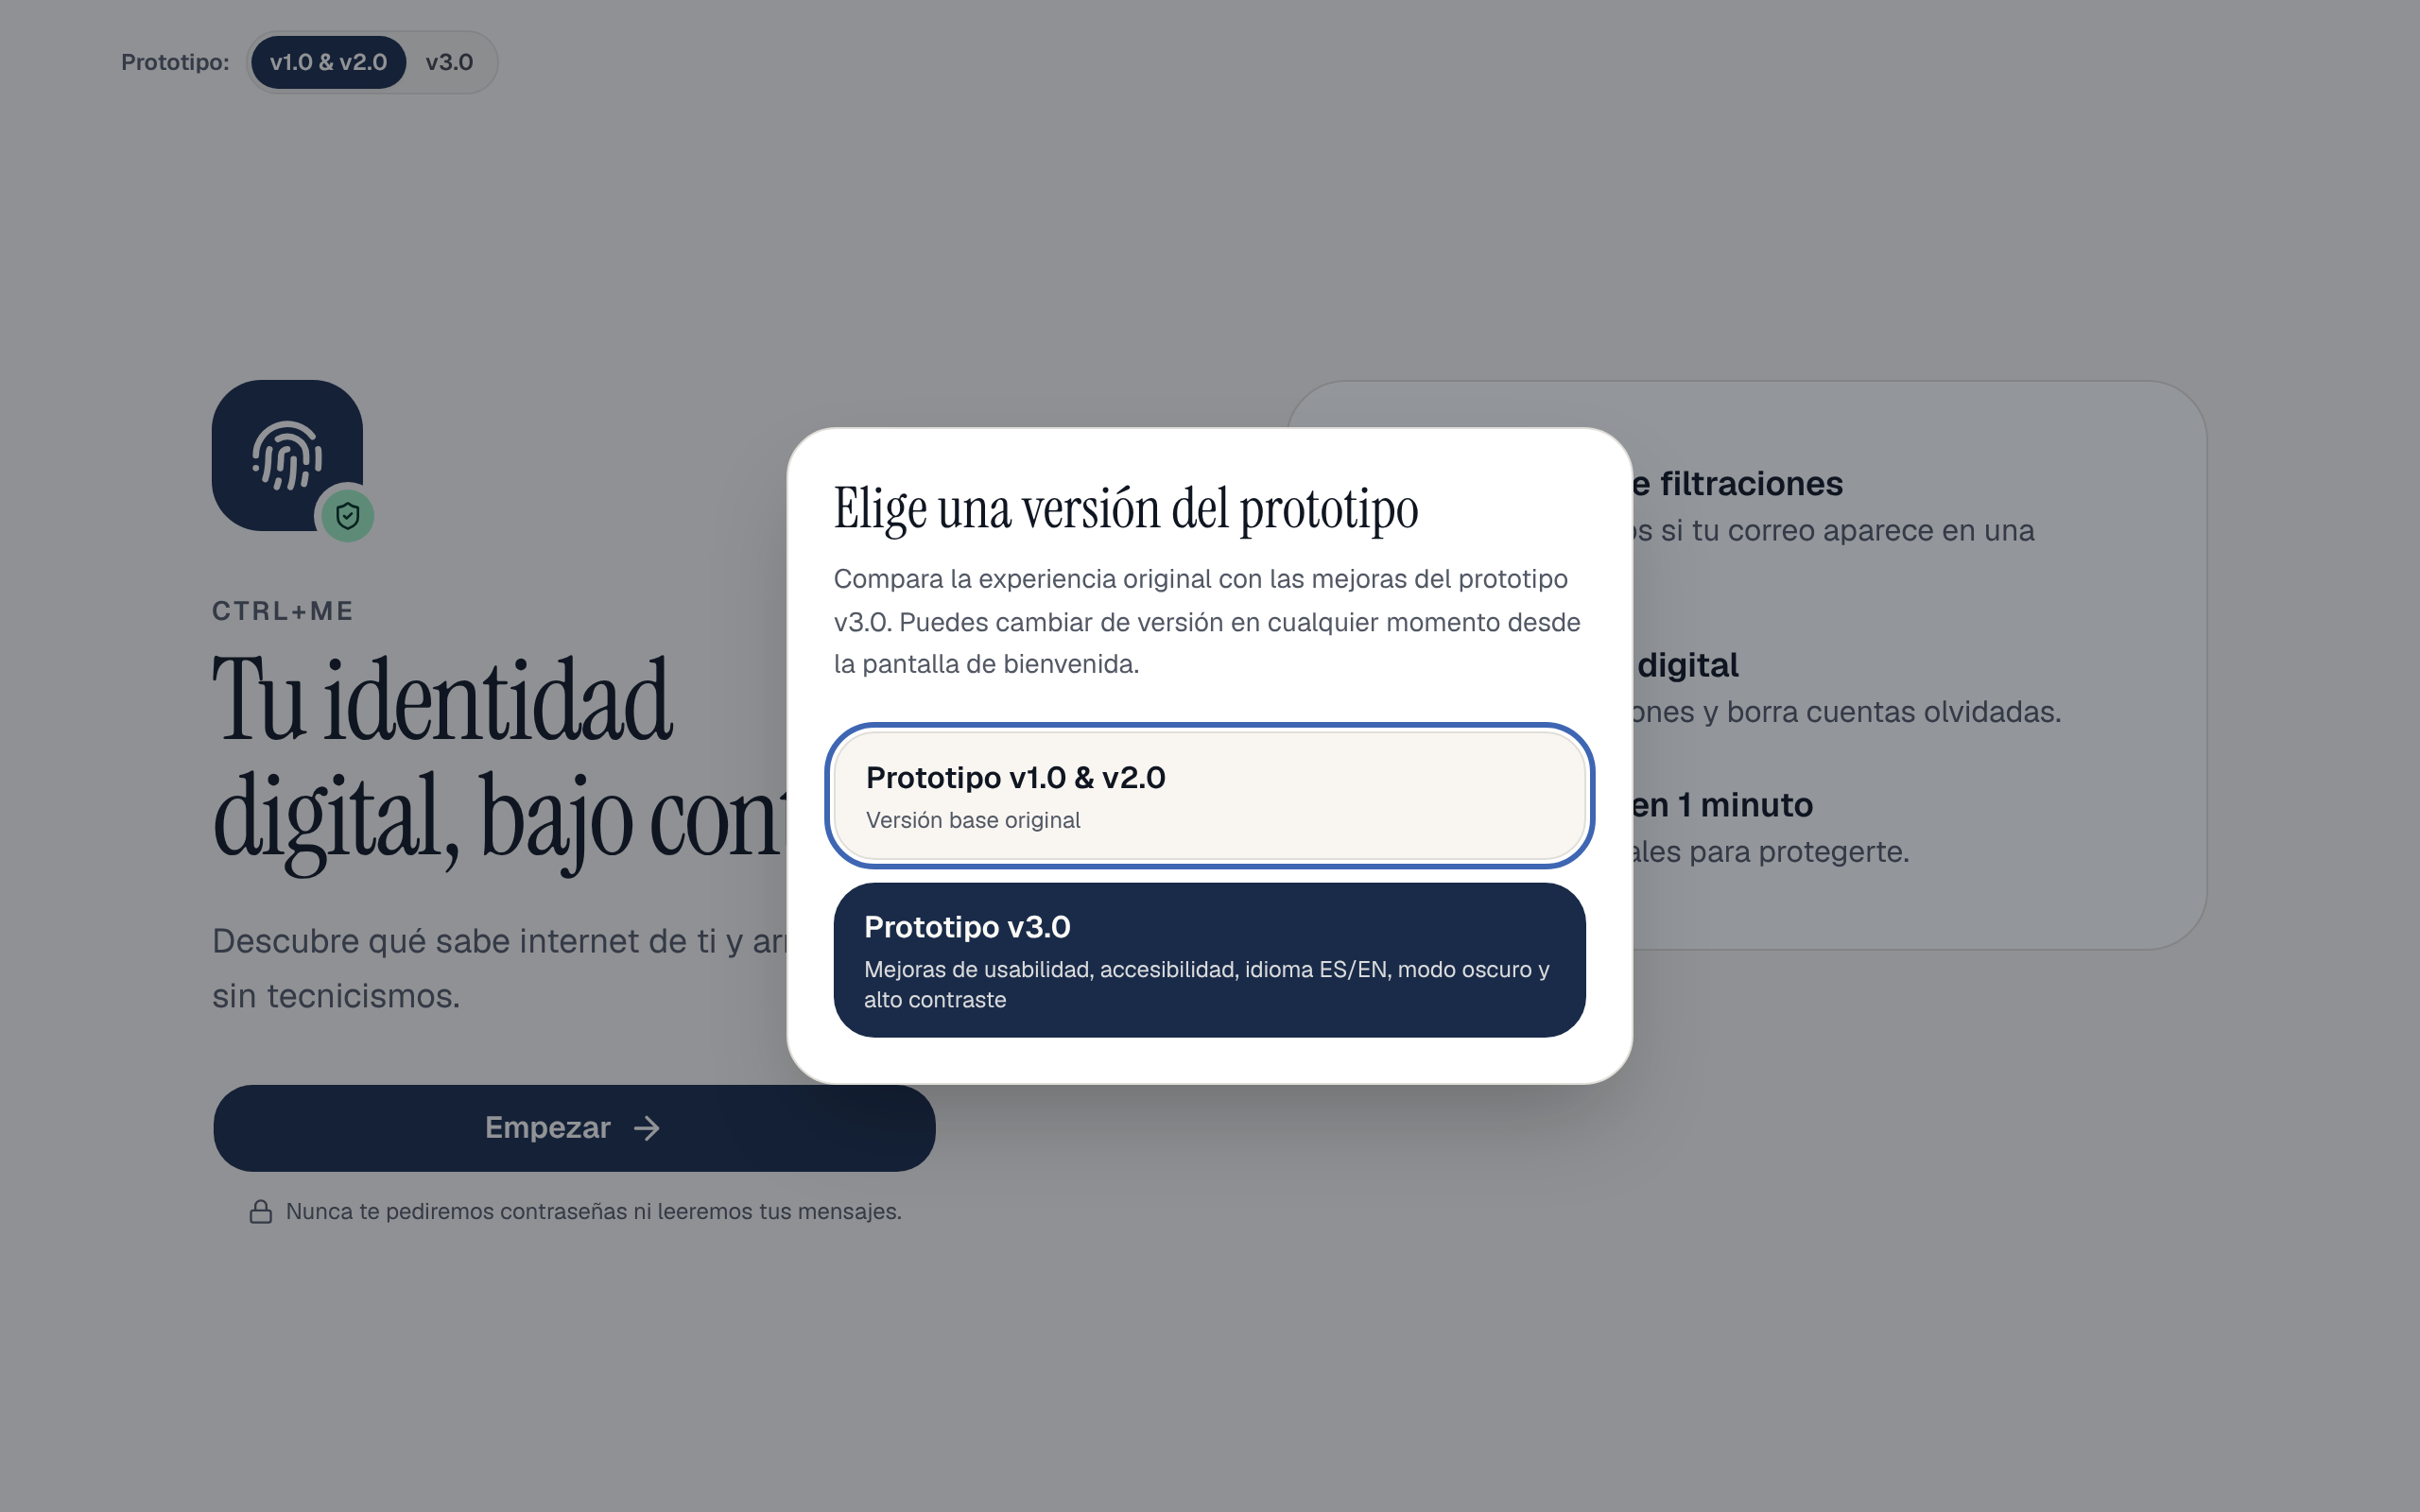
\includegraphics[width=\textwidth]{figuras-v3/v3_selector_version_web.png}
    \caption{Modal inicial de selección de versión}
    \label{fig:v3-selector-modal}
  \end{subfigure}
  \hfill
  \begin{subfigure}[b]{0.48\textwidth}
    \centering
    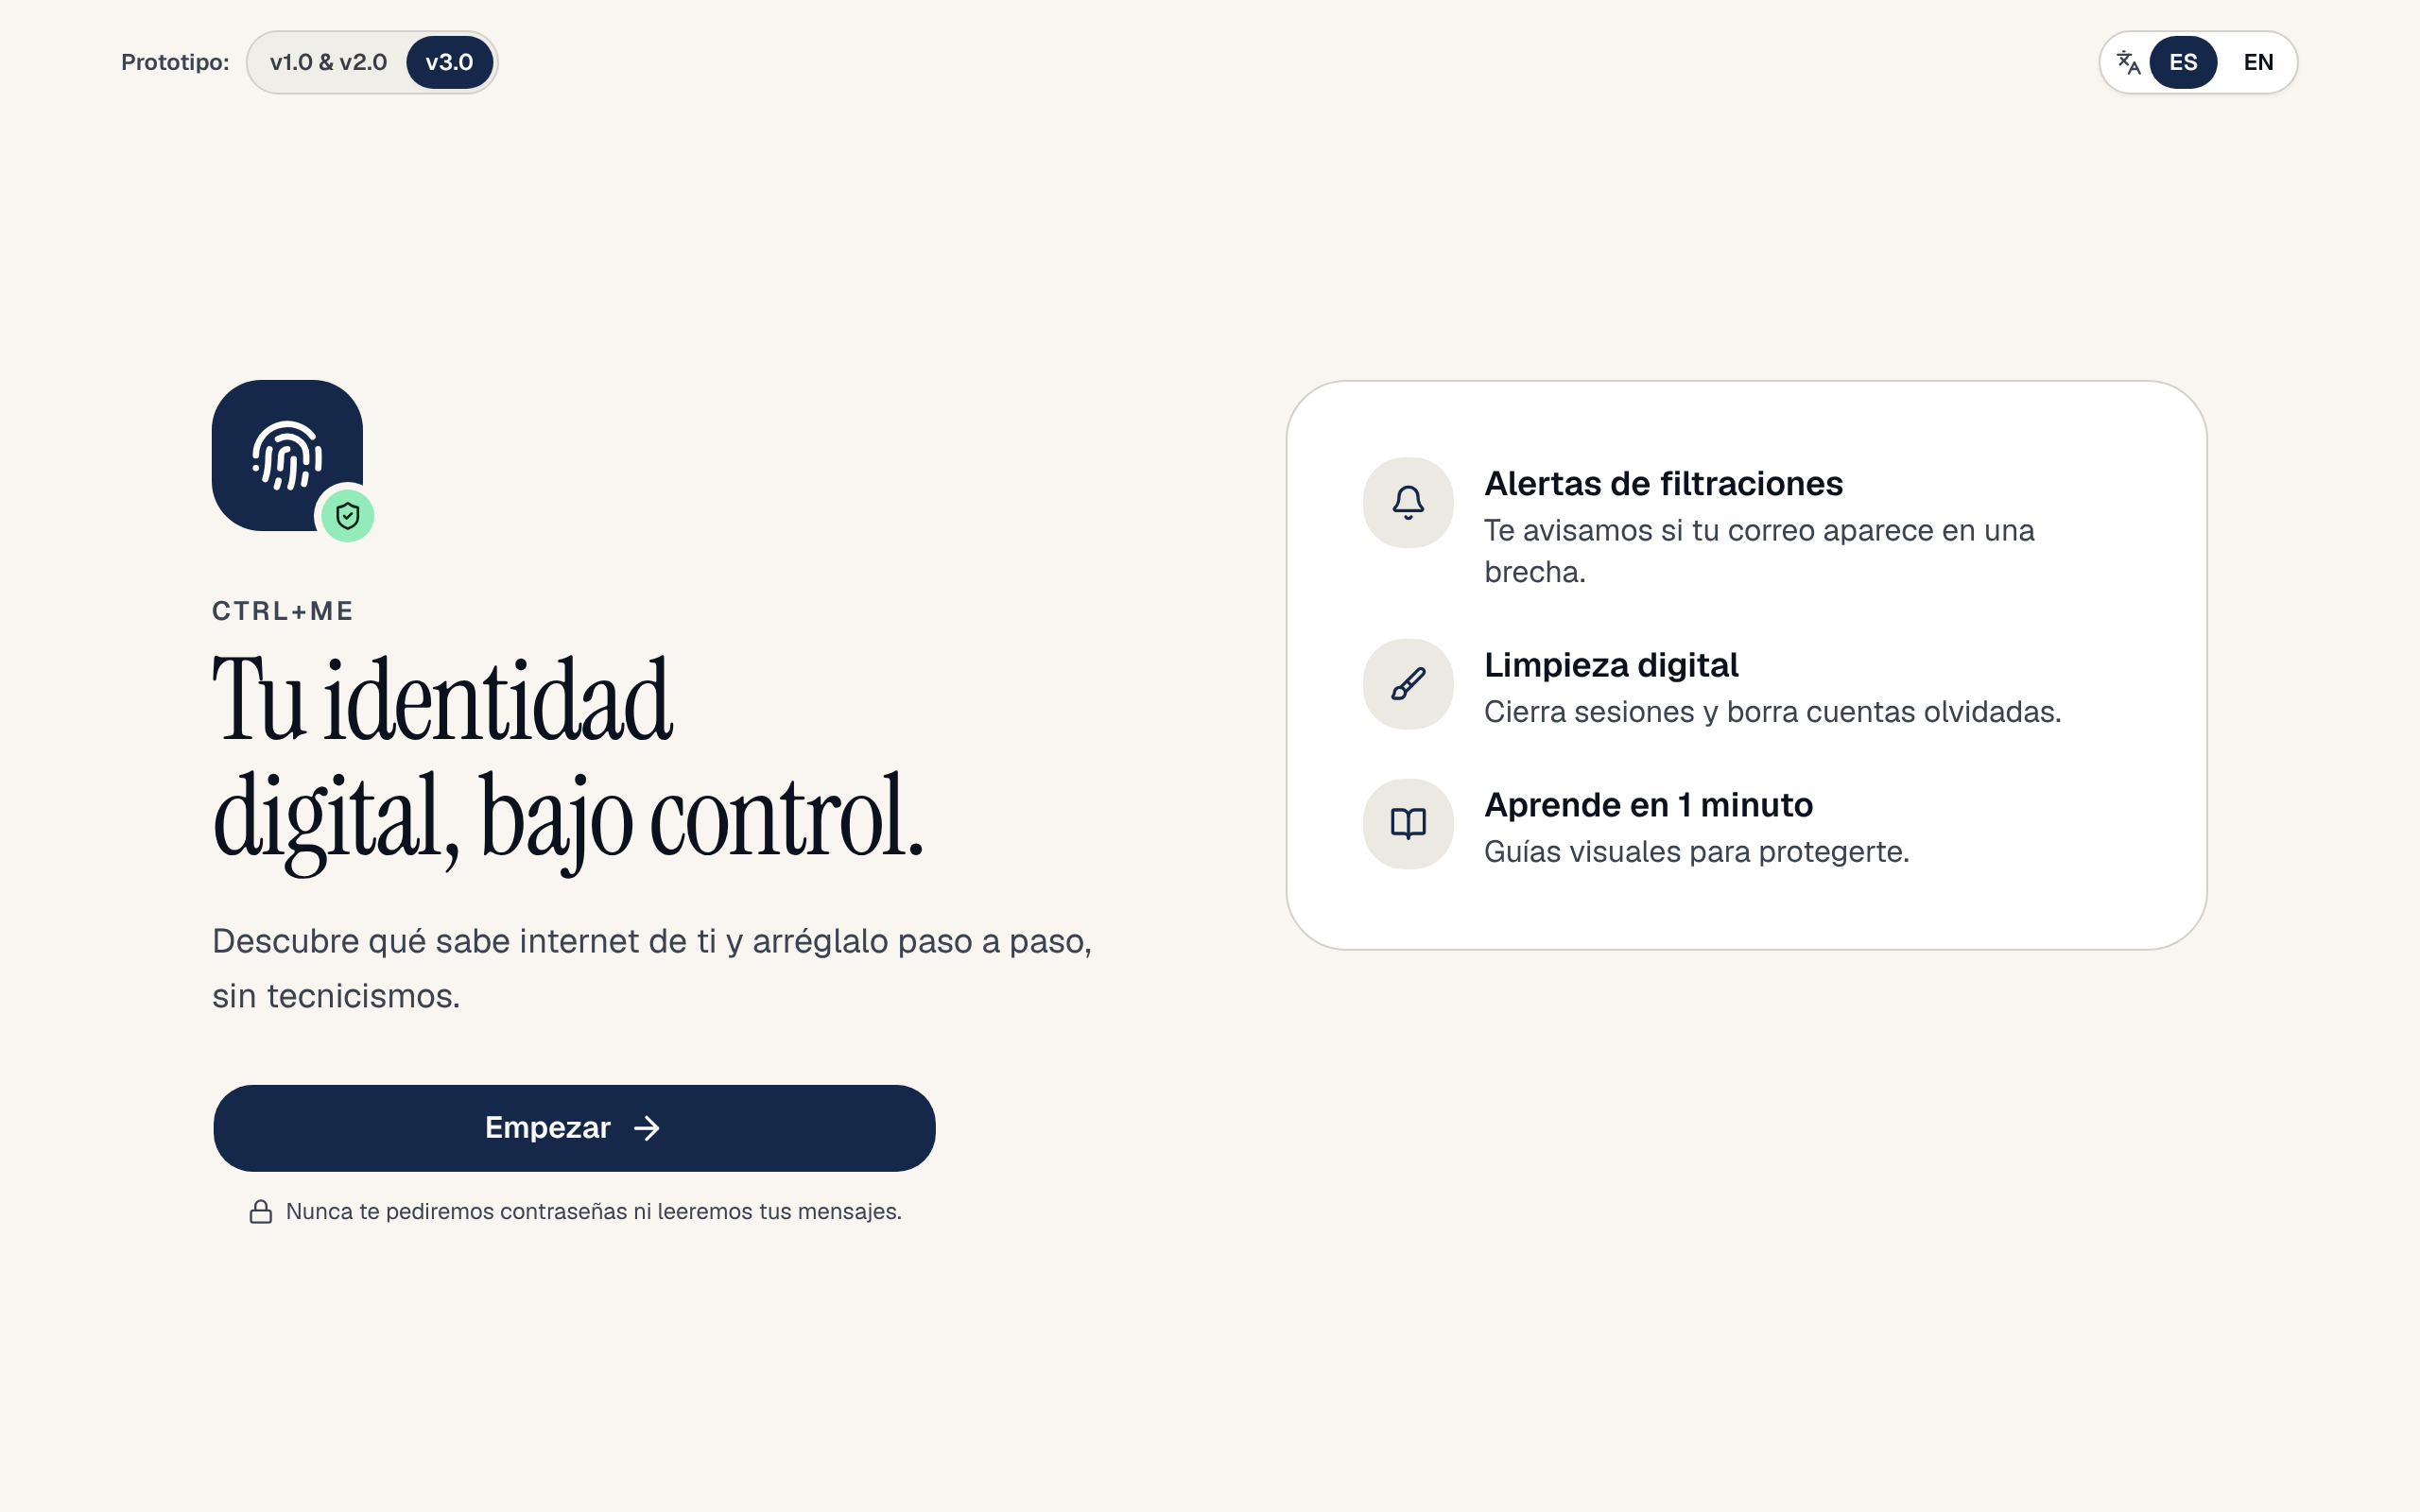
\includegraphics[width=\textwidth]{figuras-v3/v3_bienvenida_es_web.png}
    \caption{Bienvenida v3.0 con selector e idioma en barra superior}
    \label{fig:v3-bienvenida-es}
  \end{subfigure}
  \caption{Selector de prototipo en la pantalla de bienvenida (v3.0).}
  \label{fig:v3-selector-version}
\end{figure}

\subsection{Pantalla principal, consistencia visual y reducción de densidad}

La pantalla principal (\textit{Tu resumen}, Figura~\ref{fig:v3-principal}) junto a las vistas de mejora y aprendizaje (Figura~\ref{fig:v3-plan-guias}) materializan los requisitos \textbf{R-USA-1}, \textbf{R-USA-2}, \textbf{R-USA-3}, \textbf{R-USA-4} (Tabla~\ref{tab:requisitos-usabilidad}), \textbf{R-ACC-2} (Tabla~\ref{tab:requisitos-accesibilidad}) y los hallazgos de \textit{Colour Contrast Analyser} y \textit{WAVE}:

\begin{itemize}
  \item \textbf{Etiquetas inequívocas en el medidor (R-USA-1):} Se sustituyeron los calificativos genéricos \textit{Bajo}, \textit{Medio} y \textit{Alto} del arco central y su leyenda inferior por \textbf{Protección escasa} (0--59), \textbf{Protección media} (60--84) y \textbf{Protección excelente} (85--100), evitando ambigüedades con la escala de \textit{Exposición} de \textit{Tu huella digital}. Asimismo, se eliminó la atenuación de opacidad en la leyenda numérica para asegurar un contraste óptimo.
  \item \textbf{Menor densidad visual y acceso unificado (R-USA-2, R-USA-3):} Se eliminaron de la pantalla principal las tarjetas redundantes de \textit{Limpiar cuentas}, \textit{Alertas de filtraciones} y \textit{Tu plan para subir}. La acción \textbf{Mejora tu puntuación} (renombrada de forma consistente en botones, menú y cabecera) pasa a mostrarse dentro del contenedor de puntuación junto a \textbf{Ver mi huella digital}, adaptándose sin desbordamientos al 100\,\% del ancho en móvil incluso al escalar el texto al 150\,\%.
  \item \textbf{Filtrado, ordenación y coherencia cromática (R-USA-4, CCA/WAVE):} En \textit{Mejora tu puntuación} se añadieron los filtros \textbf{Todas}, \textbf{Pendientes} y \textbf{Completadas} junto al selector de ordenación por impacto. En \textit{Guías} se unificó el título \texttt{<h1>} (\textit{Guías}), se dejó \textit{Aprende en 1 minuto} como subtítulo, se reforzó el contraste de las píldoras educativas, se añadió un elemento semántico \texttt{<header>} en escritorio y se oscurecieron los textos secundarios (\texttt{--muted-foreground}).
\end{itemize}

\begin{figure}[H]
  \centering
  \begin{subfigure}[b]{0.64\textwidth}
    \centering
    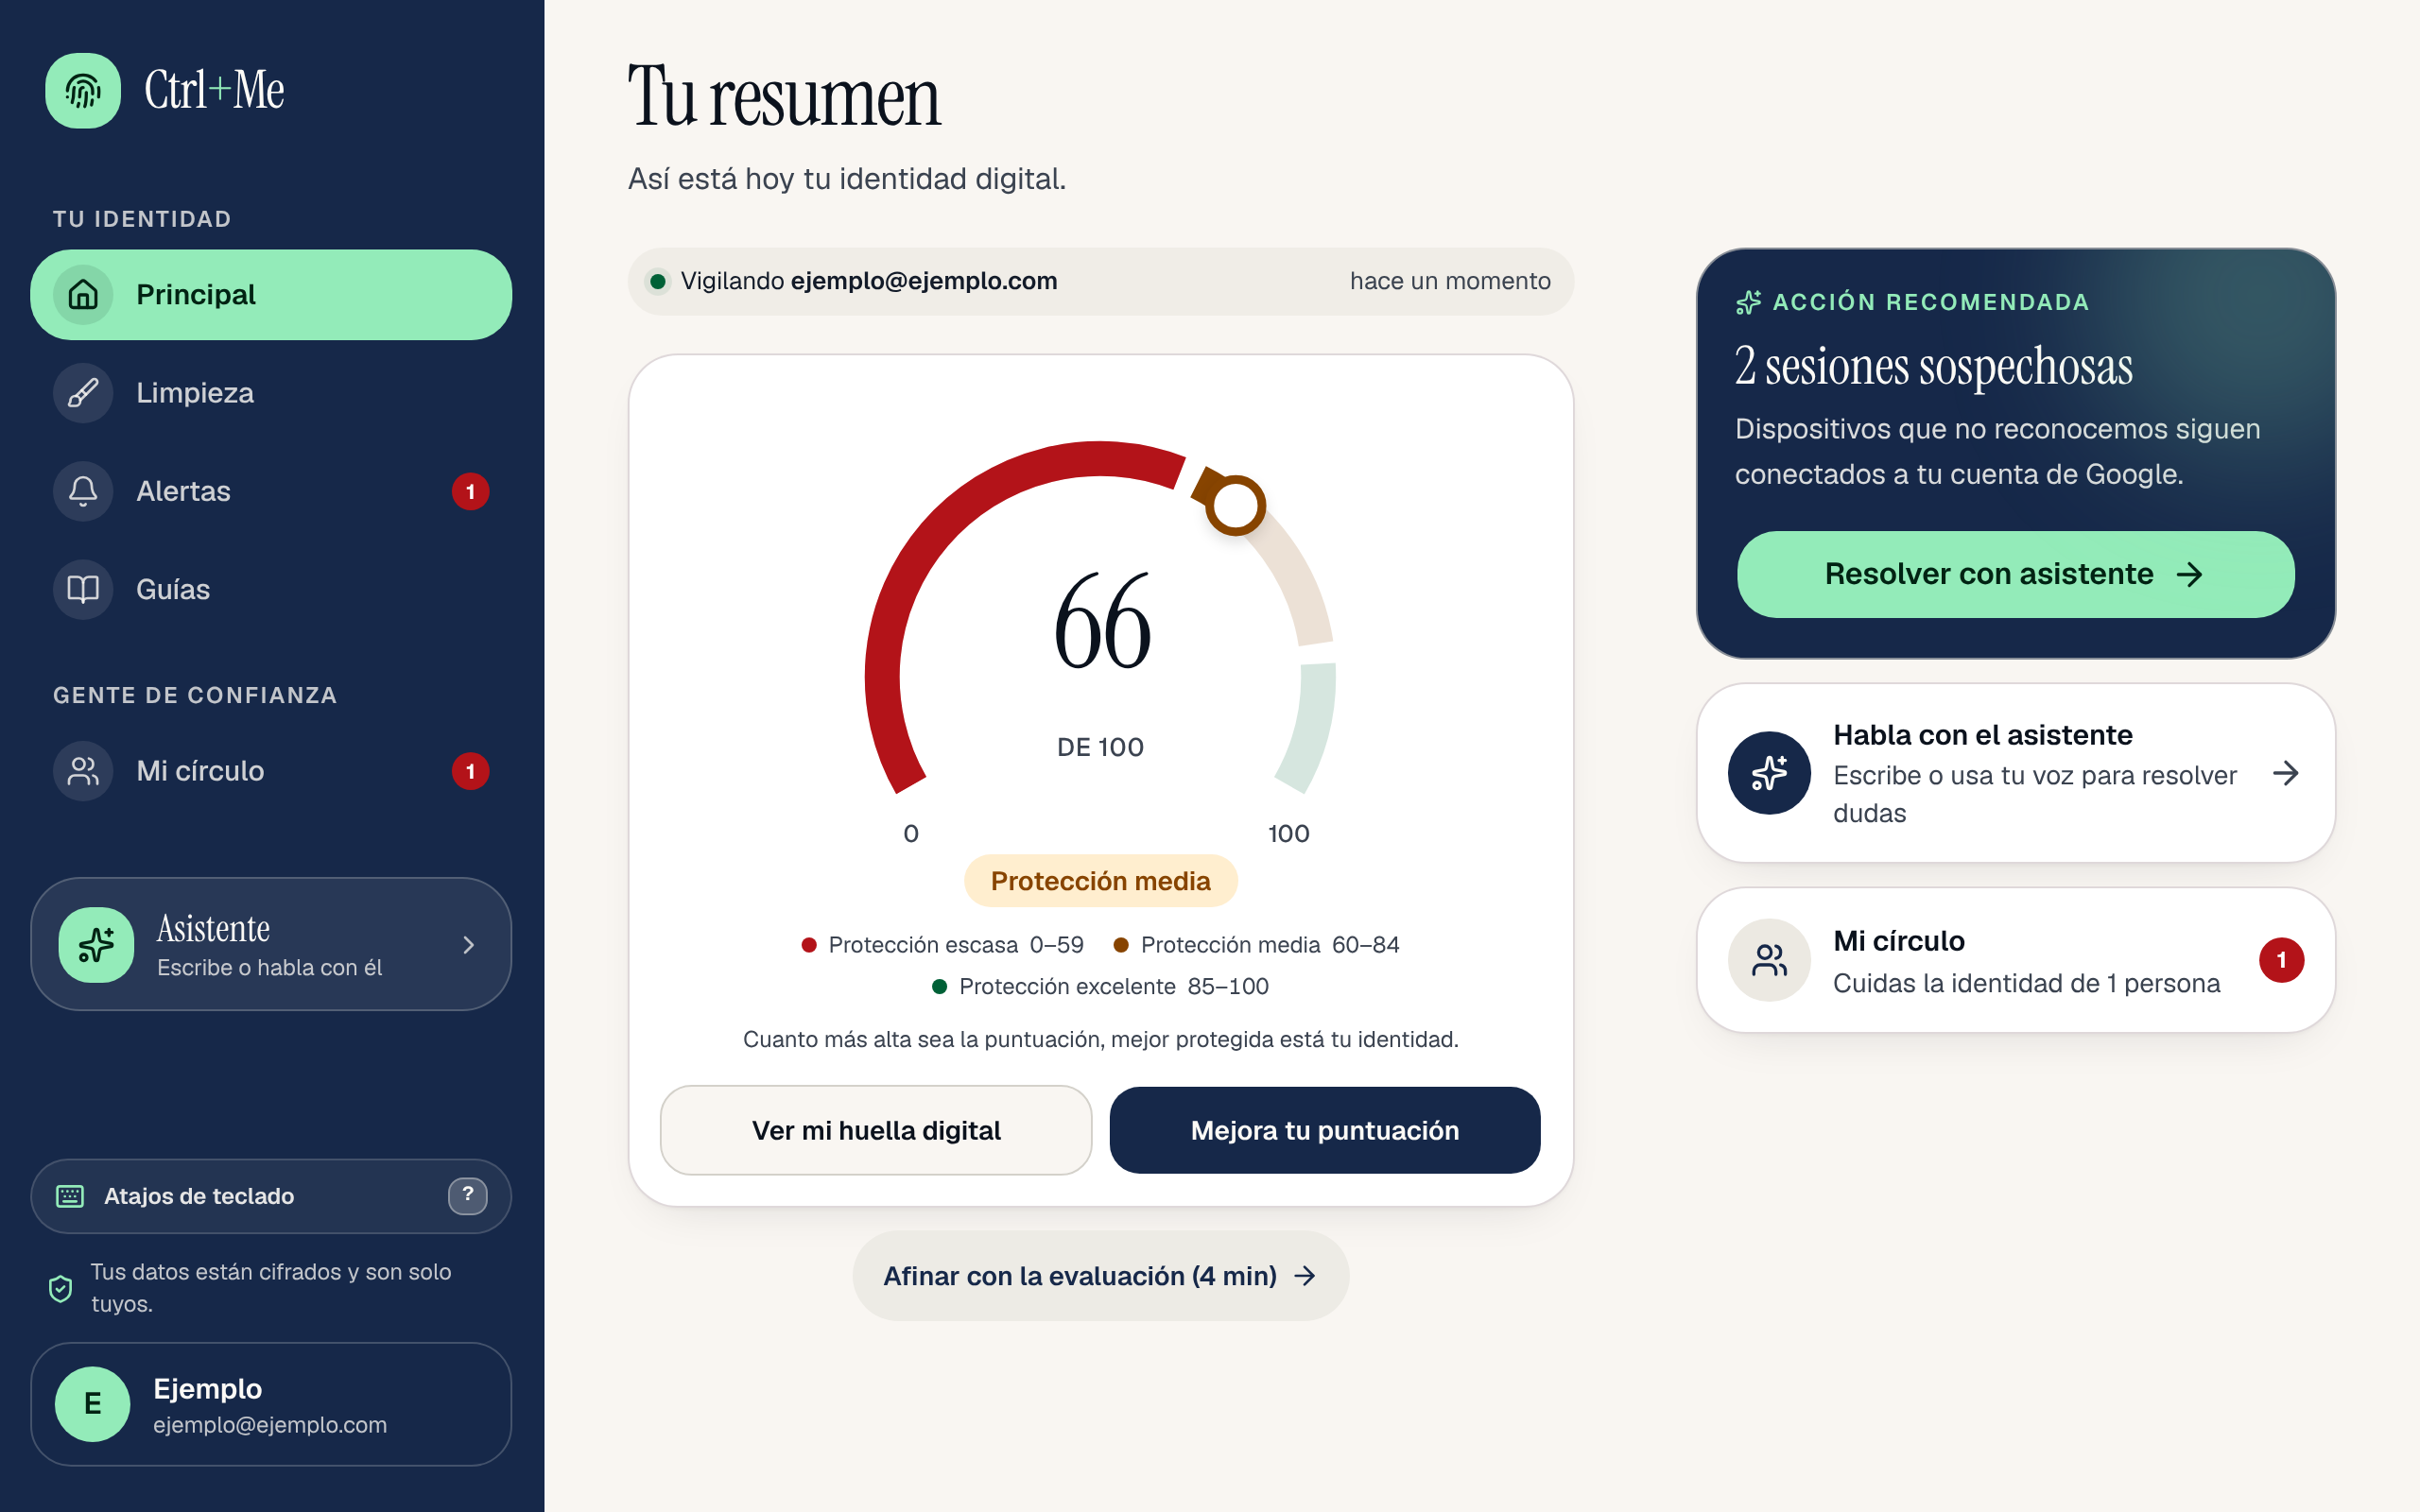
\includegraphics[width=\textwidth]{figuras-v3/v3_principal_web.png}
    \caption{Vista web con estructura \texttt{<header>} y botones integrados}
    \label{fig:v3-principal-web}
  \end{subfigure}
  \hfill
  \begin{subfigure}[b]{0.30\textwidth}
    \centering
    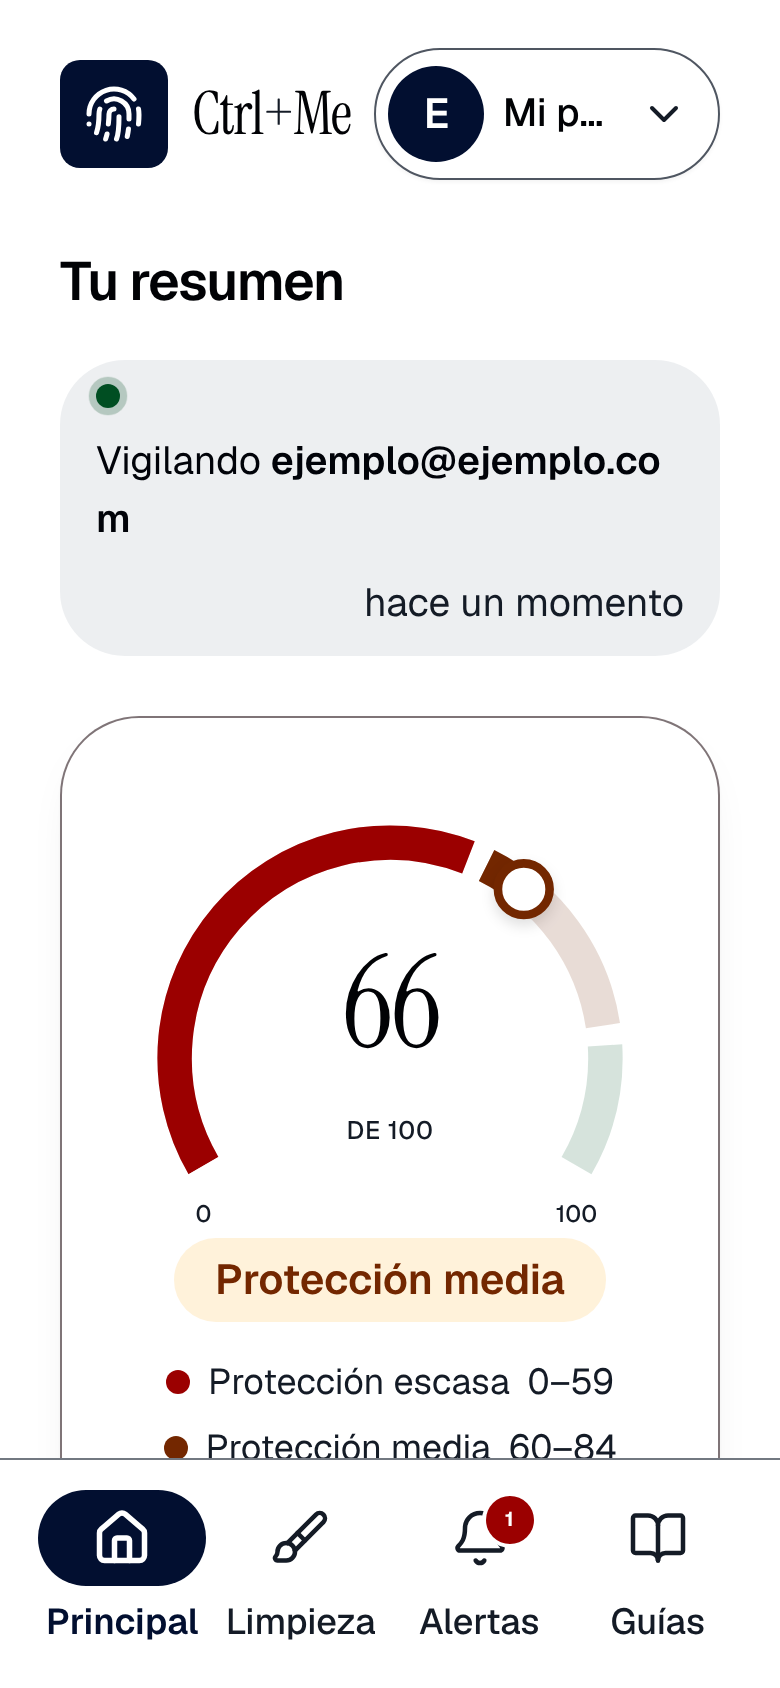
\includegraphics[width=\textwidth]{figuras-v3/v3_principal_alto_contraste_150_movil.png}
    \caption{Vista móvil (Alto contraste y texto 150\,\%)}
    \label{fig:v3-alto-contraste-150}
  \end{subfigure}
  \caption{Pantalla principal (v3.0) en escritorio y móvil con escalado accesible sin desbordamientos.}
  \label{fig:v3-principal}
\end{figure}

\begin{figure}[H]
  \centering
  \begin{subfigure}[b]{0.48\textwidth}
    \centering
    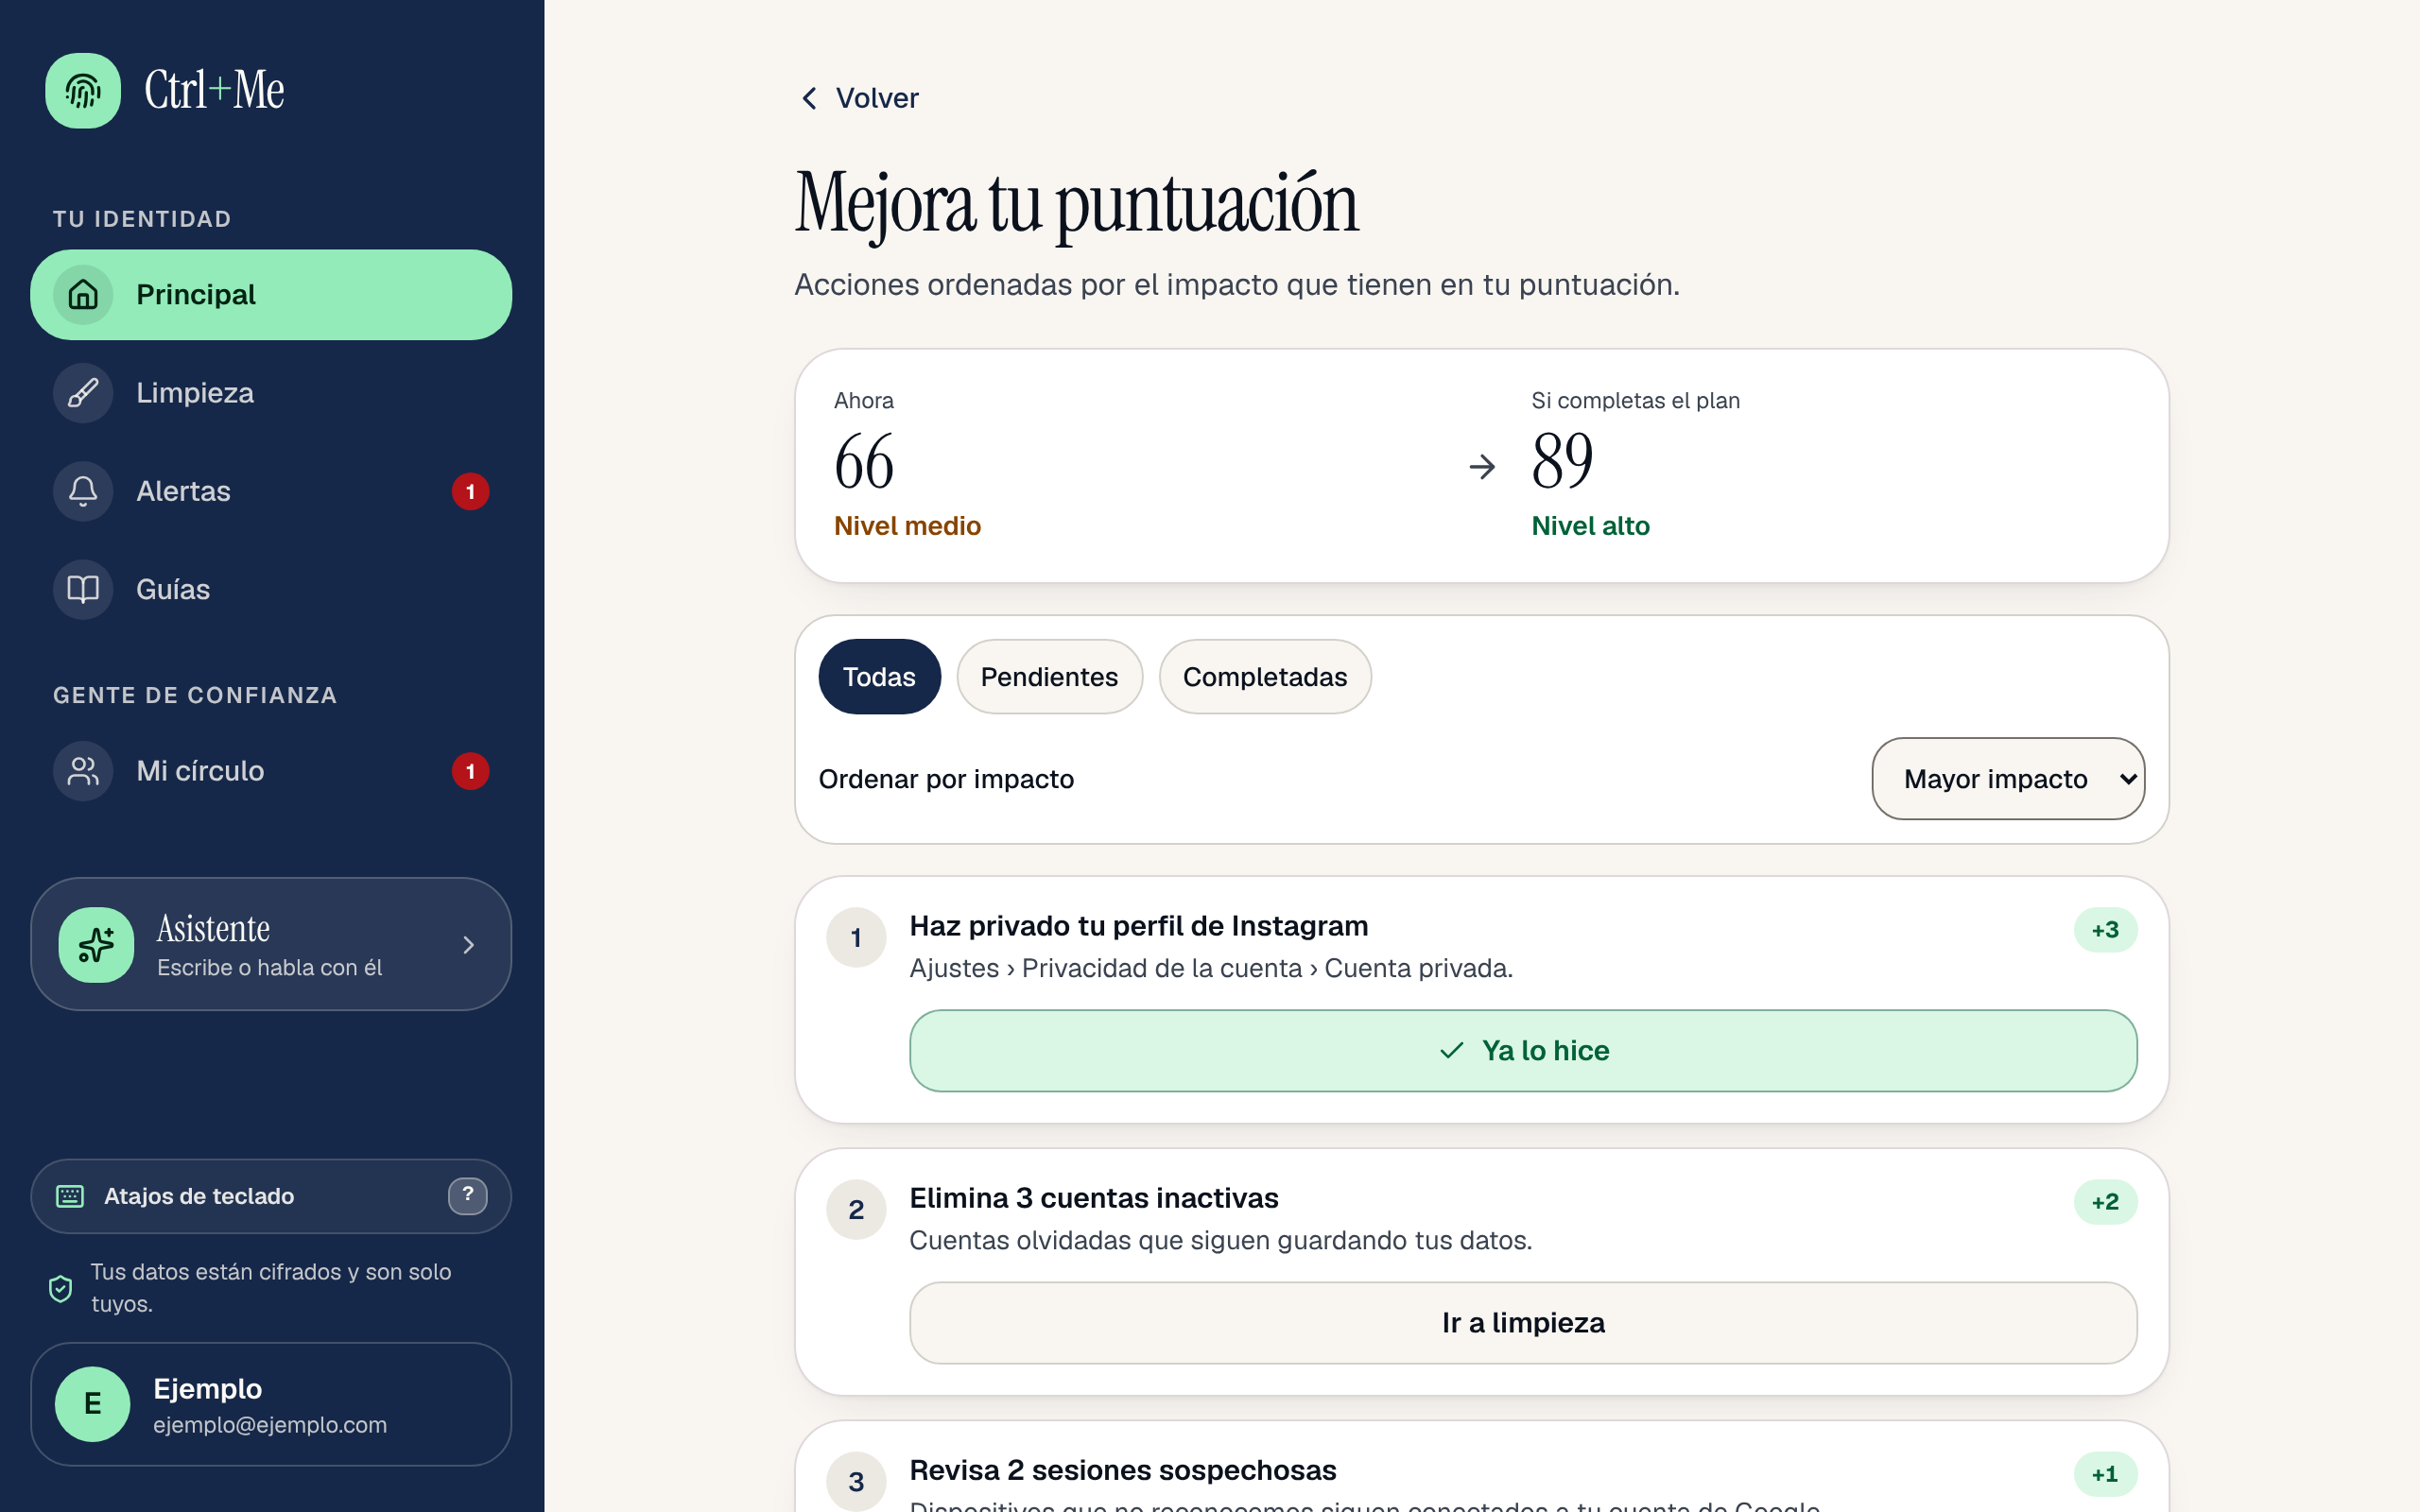
\includegraphics[width=\textwidth]{figuras-v3/v3_mejora_puntuacion_web.png}
    \caption{Mejora tu puntuación con filtros y ordenación}
    \label{fig:v3-plan-web}
  \end{subfigure}
  \hfill
  \begin{subfigure}[b]{0.48\textwidth}
    \centering
    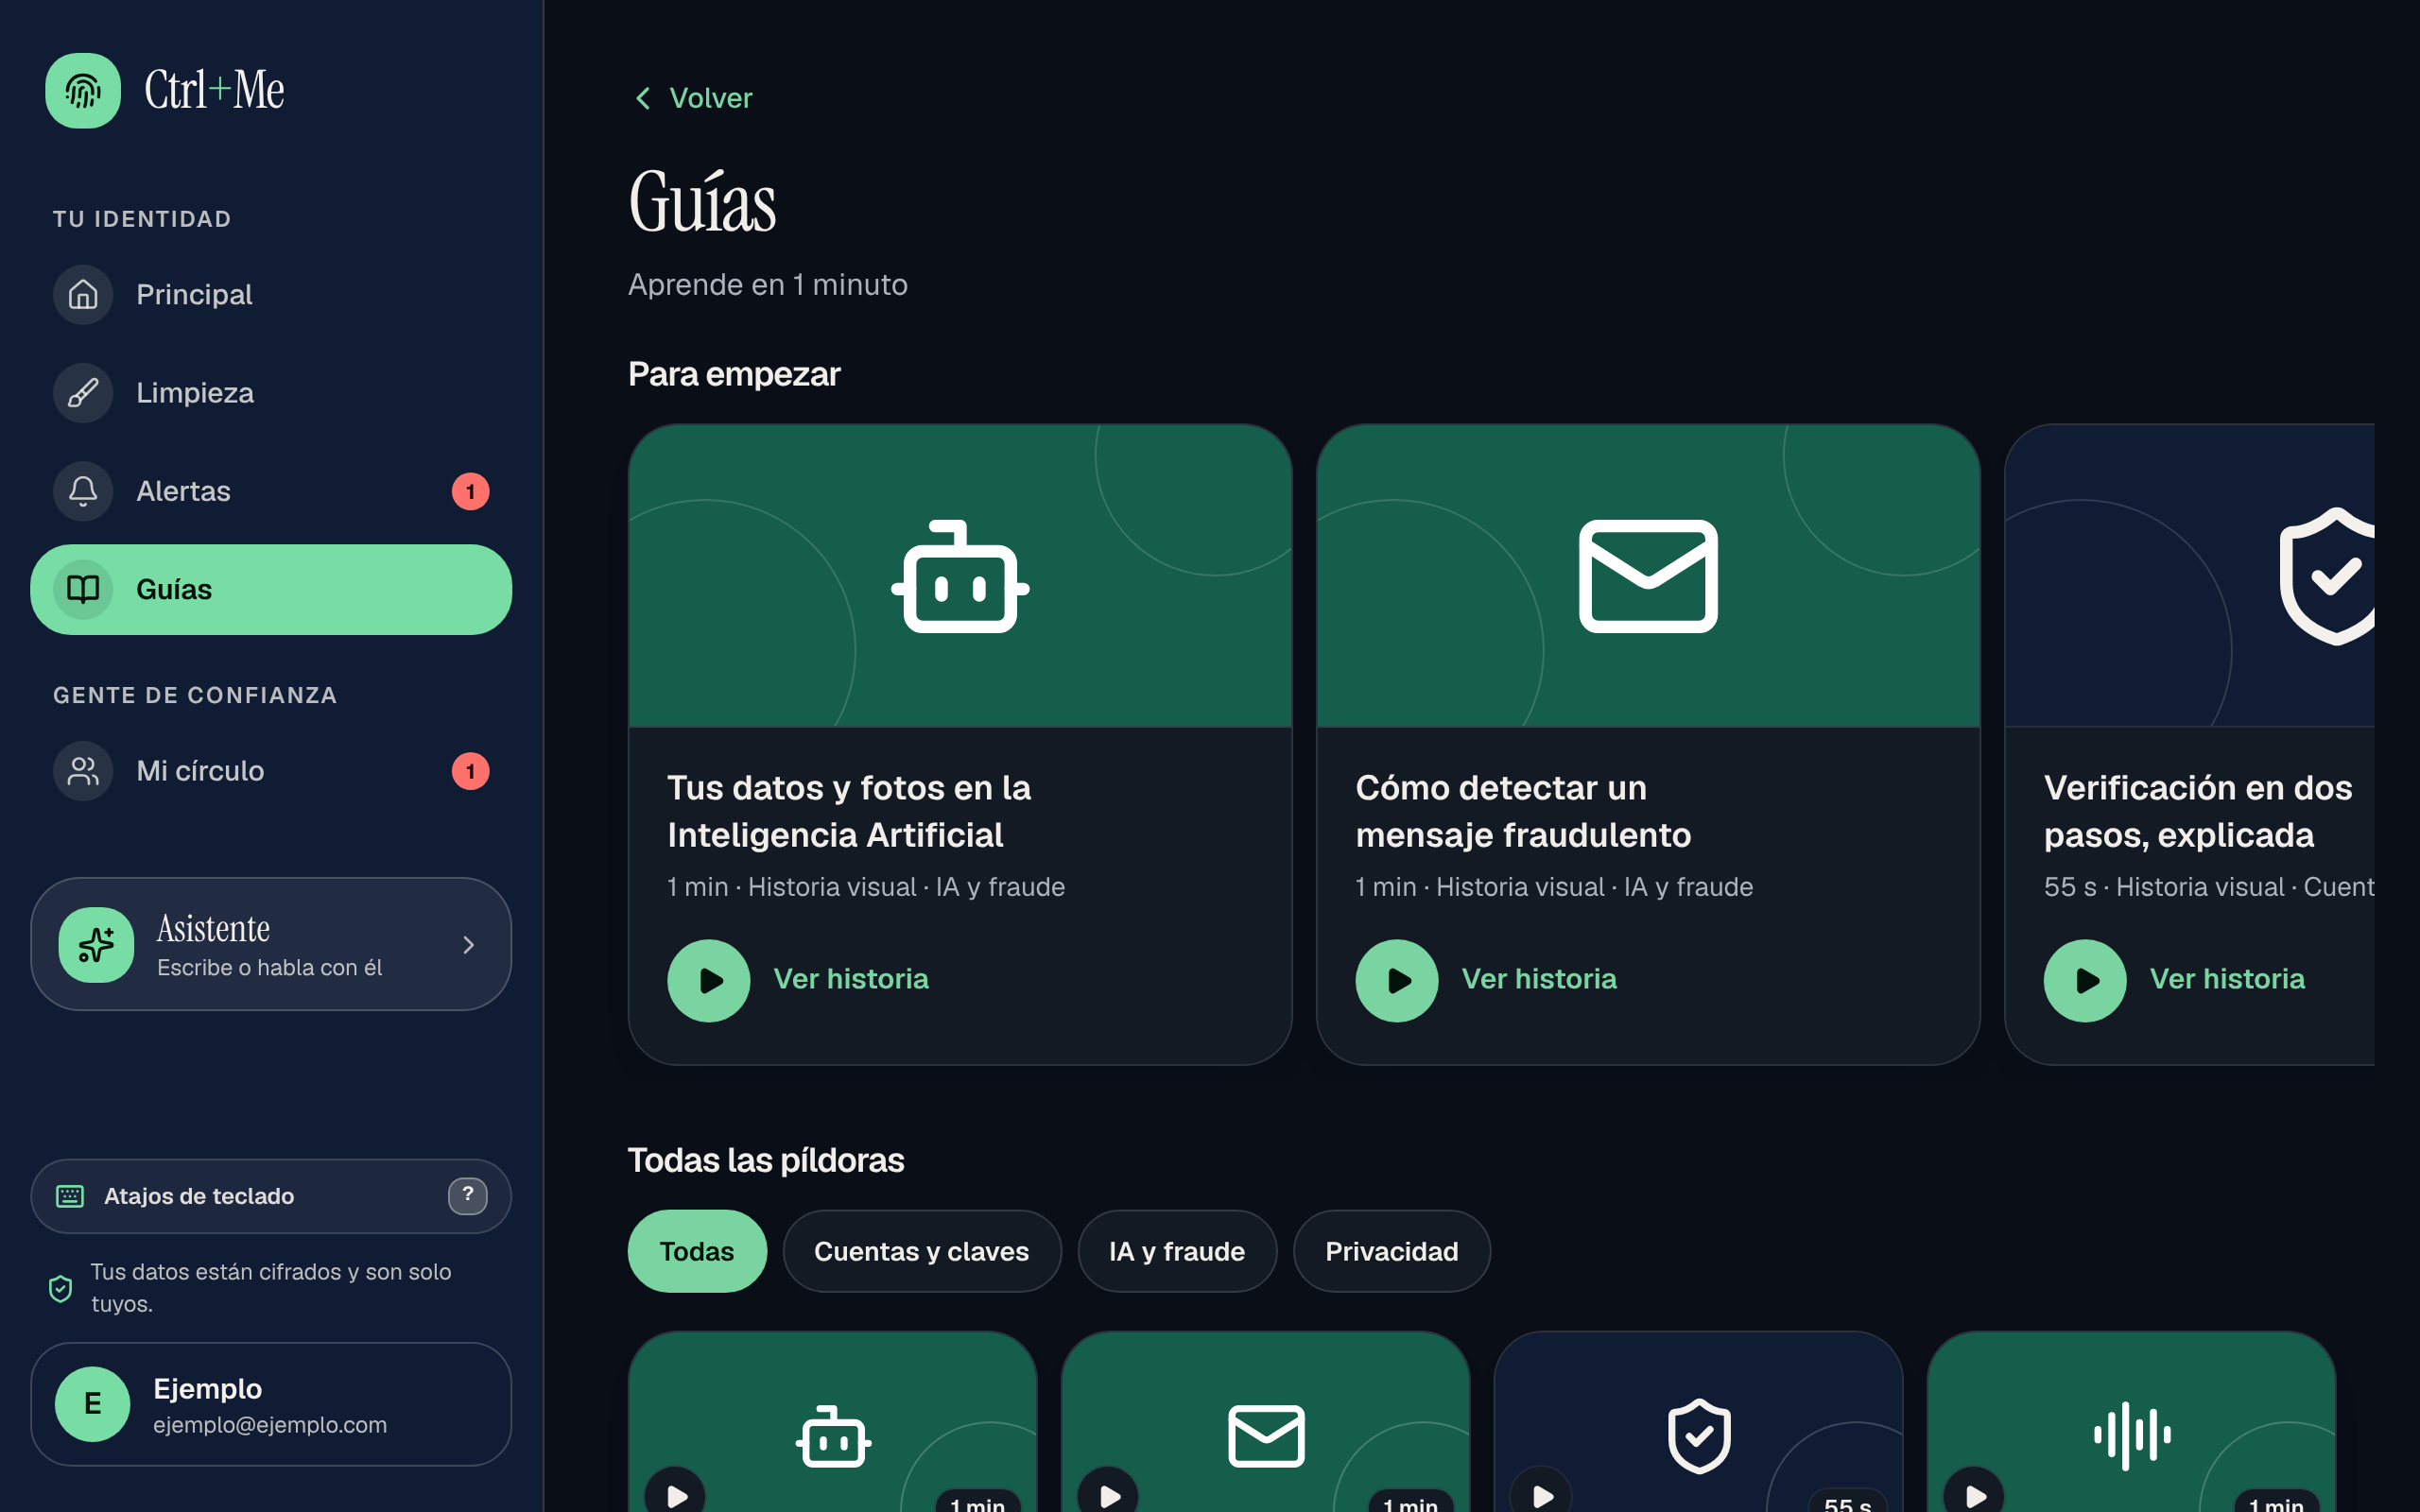
\includegraphics[width=\textwidth]{figuras-v3/v3_guias_oscuro_web.png}
    \caption{Guías en modo oscuro con título unificado}
    \label{fig:v3-guias-oscuro-web}
  \end{subfigure}
  \caption{Consistencia en \textit{Mejora tu puntuación} y \textit{Guías} (v3.0), incluyendo tema oscuro.}
  \label{fig:v3-plan-guias}
\end{figure}

\subsection{Registro, autoguardado, errores con foco y atajos de teclado}

Para reforzar la robustez ante errores, la confianza durante los cuestionarios y la agilidad con teclado (Figuras~\ref{fig:v3-errores-autoguardado} y~\ref{fig:v3-seguridad-atajos}), se aplicaron los requisitos \textbf{R-USA-5}, \textbf{R-USA-6}, \textbf{R-USA-7}, \textbf{R-USA-8} y \textbf{R-ACC-1}:

\begin{itemize}
  \item \textbf{Gestión de errores y traslado automático de foco (R-USA-7, accesibilidad de formularios):} En el paso 1 del registro, al enviar el formulario con un correo inválido o sin marcar la casilla de autorización, la interfaz muestra el mensaje de error junto al campo y desplaza de inmediato el foco y el indicador visual de enfoque al primer elemento erróneo. En el paso 2, el código \texttt{000000} muestra una alerta roja inline con acciones de recuperación (\textit{Reenviar código} y \textit{Cambiar correo}). Asimismo, ante fallos de conexión se presenta un aviso superior descartable con botón \textbf{Reintentar}.
  \item \textbf{Autoguardado continuo en evaluación (R-USA-8):} Todos los pasos de \textit{Evaluación de huella} muestran el indicador \textbf{Guardado automático} con confirmación visual y homogeneizan el contraste de controles tipo radio y segmentados.
  \item \textbf{Atajos de teclado y confirmaciones modales (R-USA-5, R-USA-6):} En escritorio se integran \texttt{Shift+1..5} para cambiar de sección, \texttt{?} para abrir el diálogo renovado de \textbf{Atajos de teclado} desde cualquier pantalla (oculto en móvil para evitar solapamientos) y \texttt{Esc} para cerrar ventanas modales. Las acciones críticas (\textit{Borrar mis datos y cuenta} y \textit{Retirar su acceso}) exigen confirmación en un diálogo modal (\texttt{alertdialog}).
\end{itemize}

\begin{figure}[H]
  \centering
  \begin{subfigure}[b]{0.27\textwidth}
    \centering
    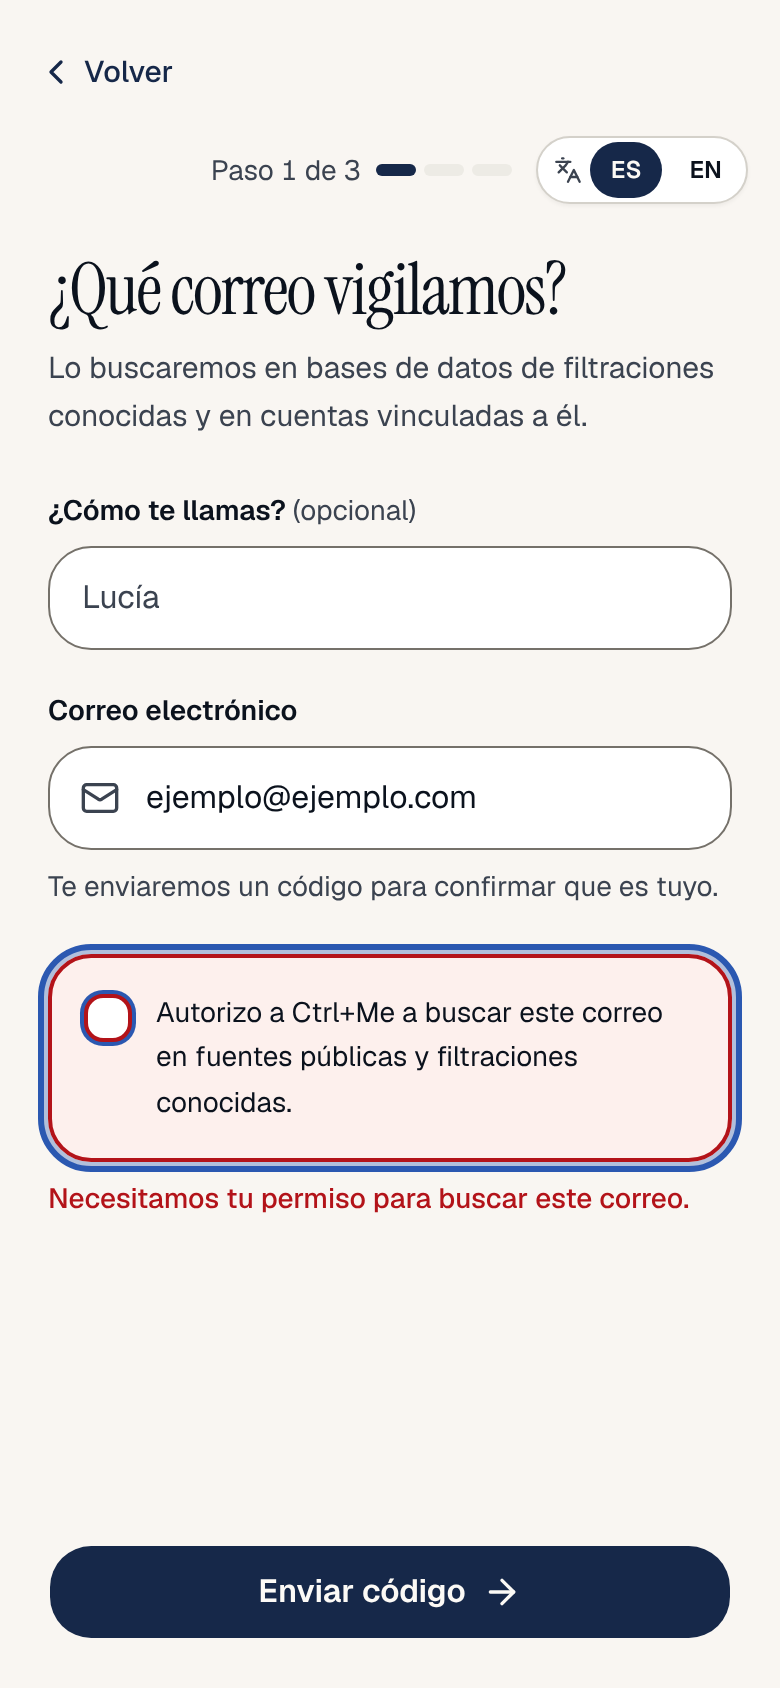
\includegraphics[width=\textwidth]{figuras-v3/v3_onboarding_error_checkbox_movil.png}
    \caption{Error y traslado de foco al campo pendiente (Paso 1)}
    \label{fig:v3-error-foco-movil}
  \end{subfigure}
  \hfill
  \begin{subfigure}[b]{0.27\textwidth}
    \centering
    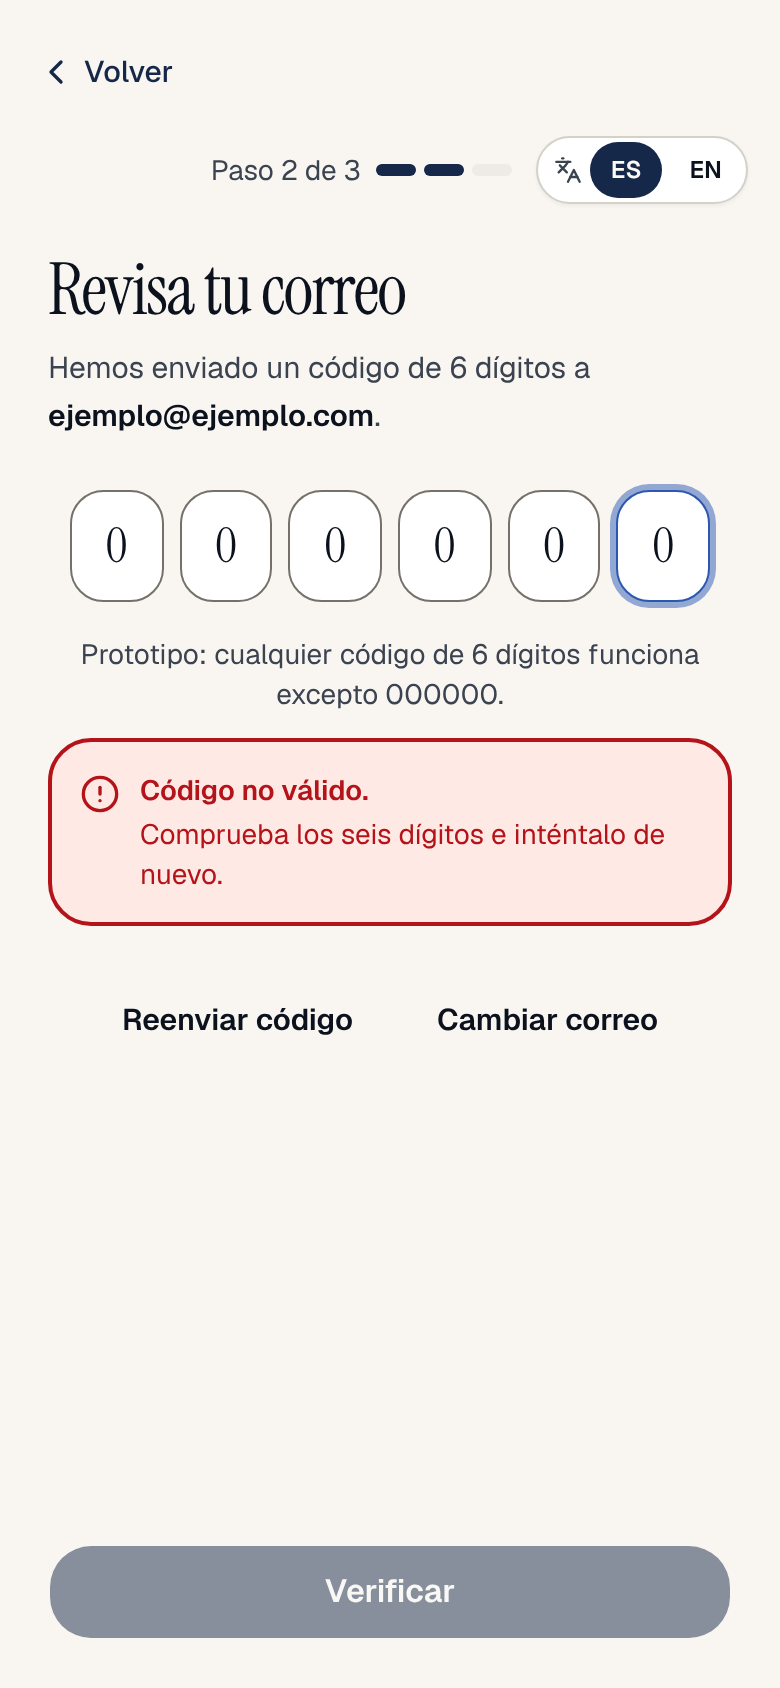
\includegraphics[width=\textwidth]{figuras-v3/v3_onboarding_error_codigo_movil.png}
    \caption{Error inline de código inválido (Paso 2)}
    \label{fig:v3-error-codigo-movil}
  \end{subfigure}
  \hfill
  \begin{subfigure}[b]{0.42\textwidth}
    \centering
    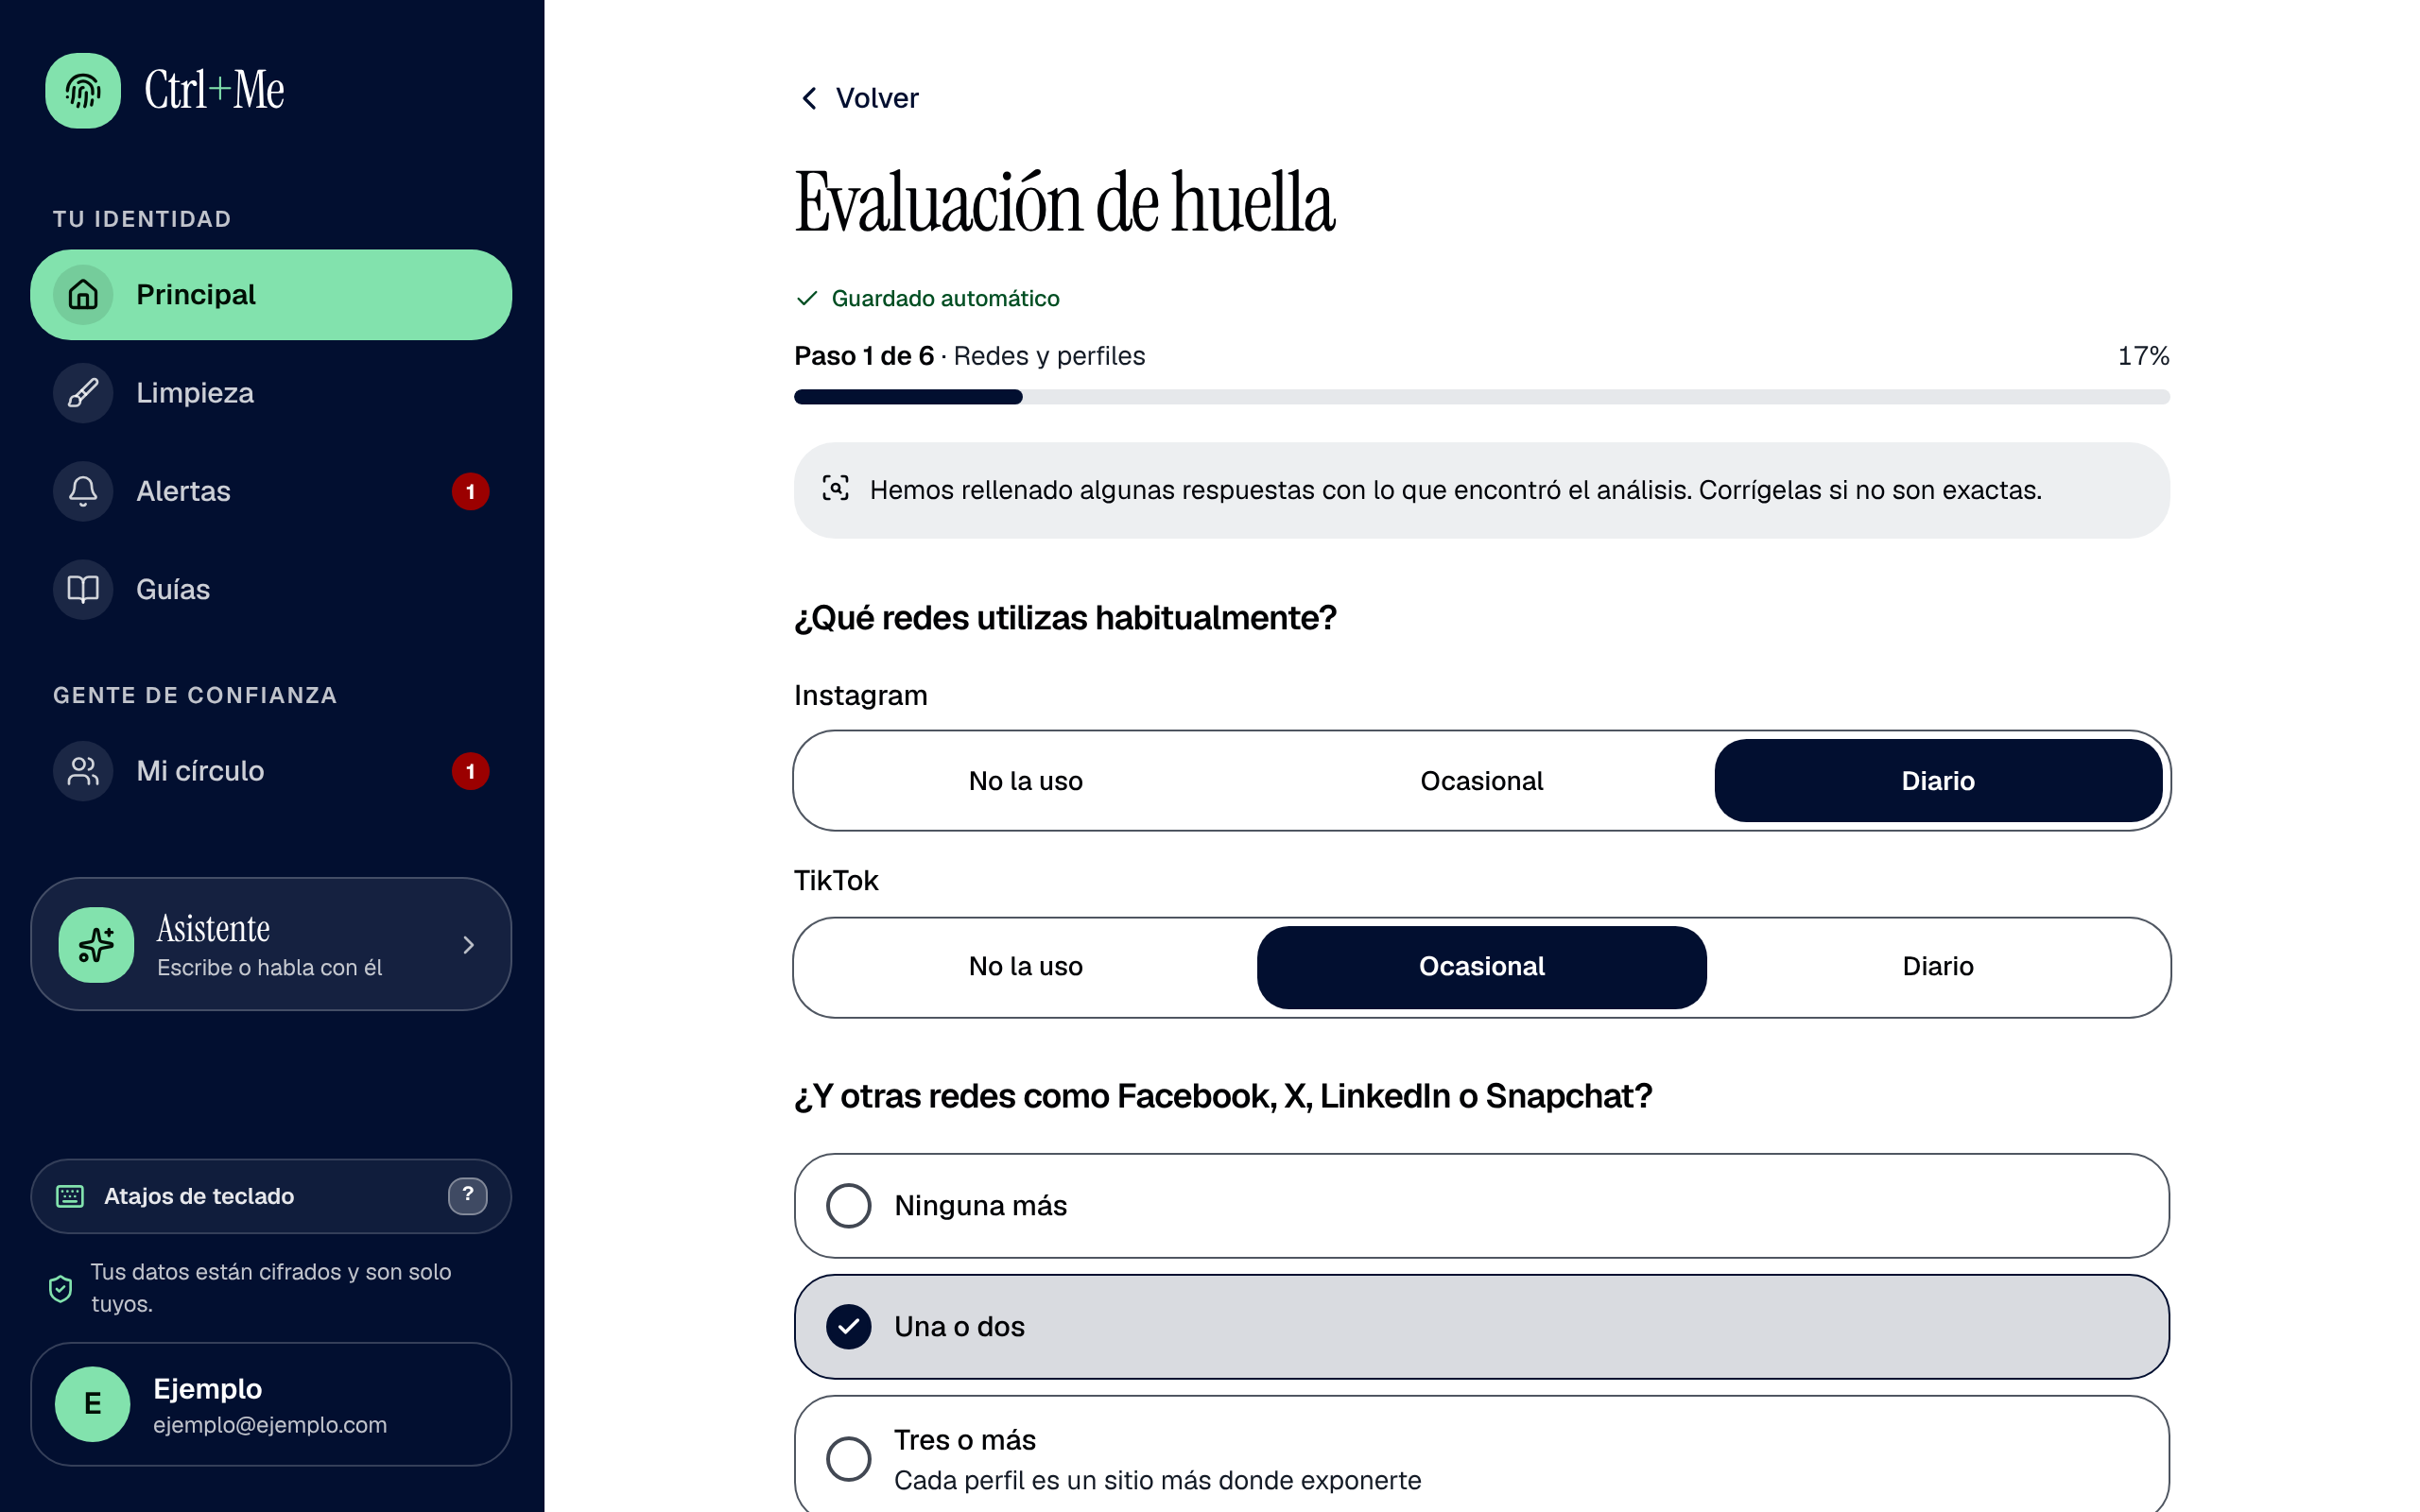
\includegraphics[width=\textwidth]{figuras-v3/v3_evaluacion_claro_alto_contraste_web.png}
    \caption{Evaluación (Alto contraste + autoguardado)}
    \label{fig:v3-evaluacion-ac-web}
  \end{subfigure}
  \caption{Traslado visible de foco ante errores en registro, validación de código y autoguardado continuo (v3.0).}
  \label{fig:v3-errores-autoguardado}
\end{figure}

\begin{figure}[H]
  \centering
  \begin{subfigure}[b]{0.48\textwidth}
    \centering
    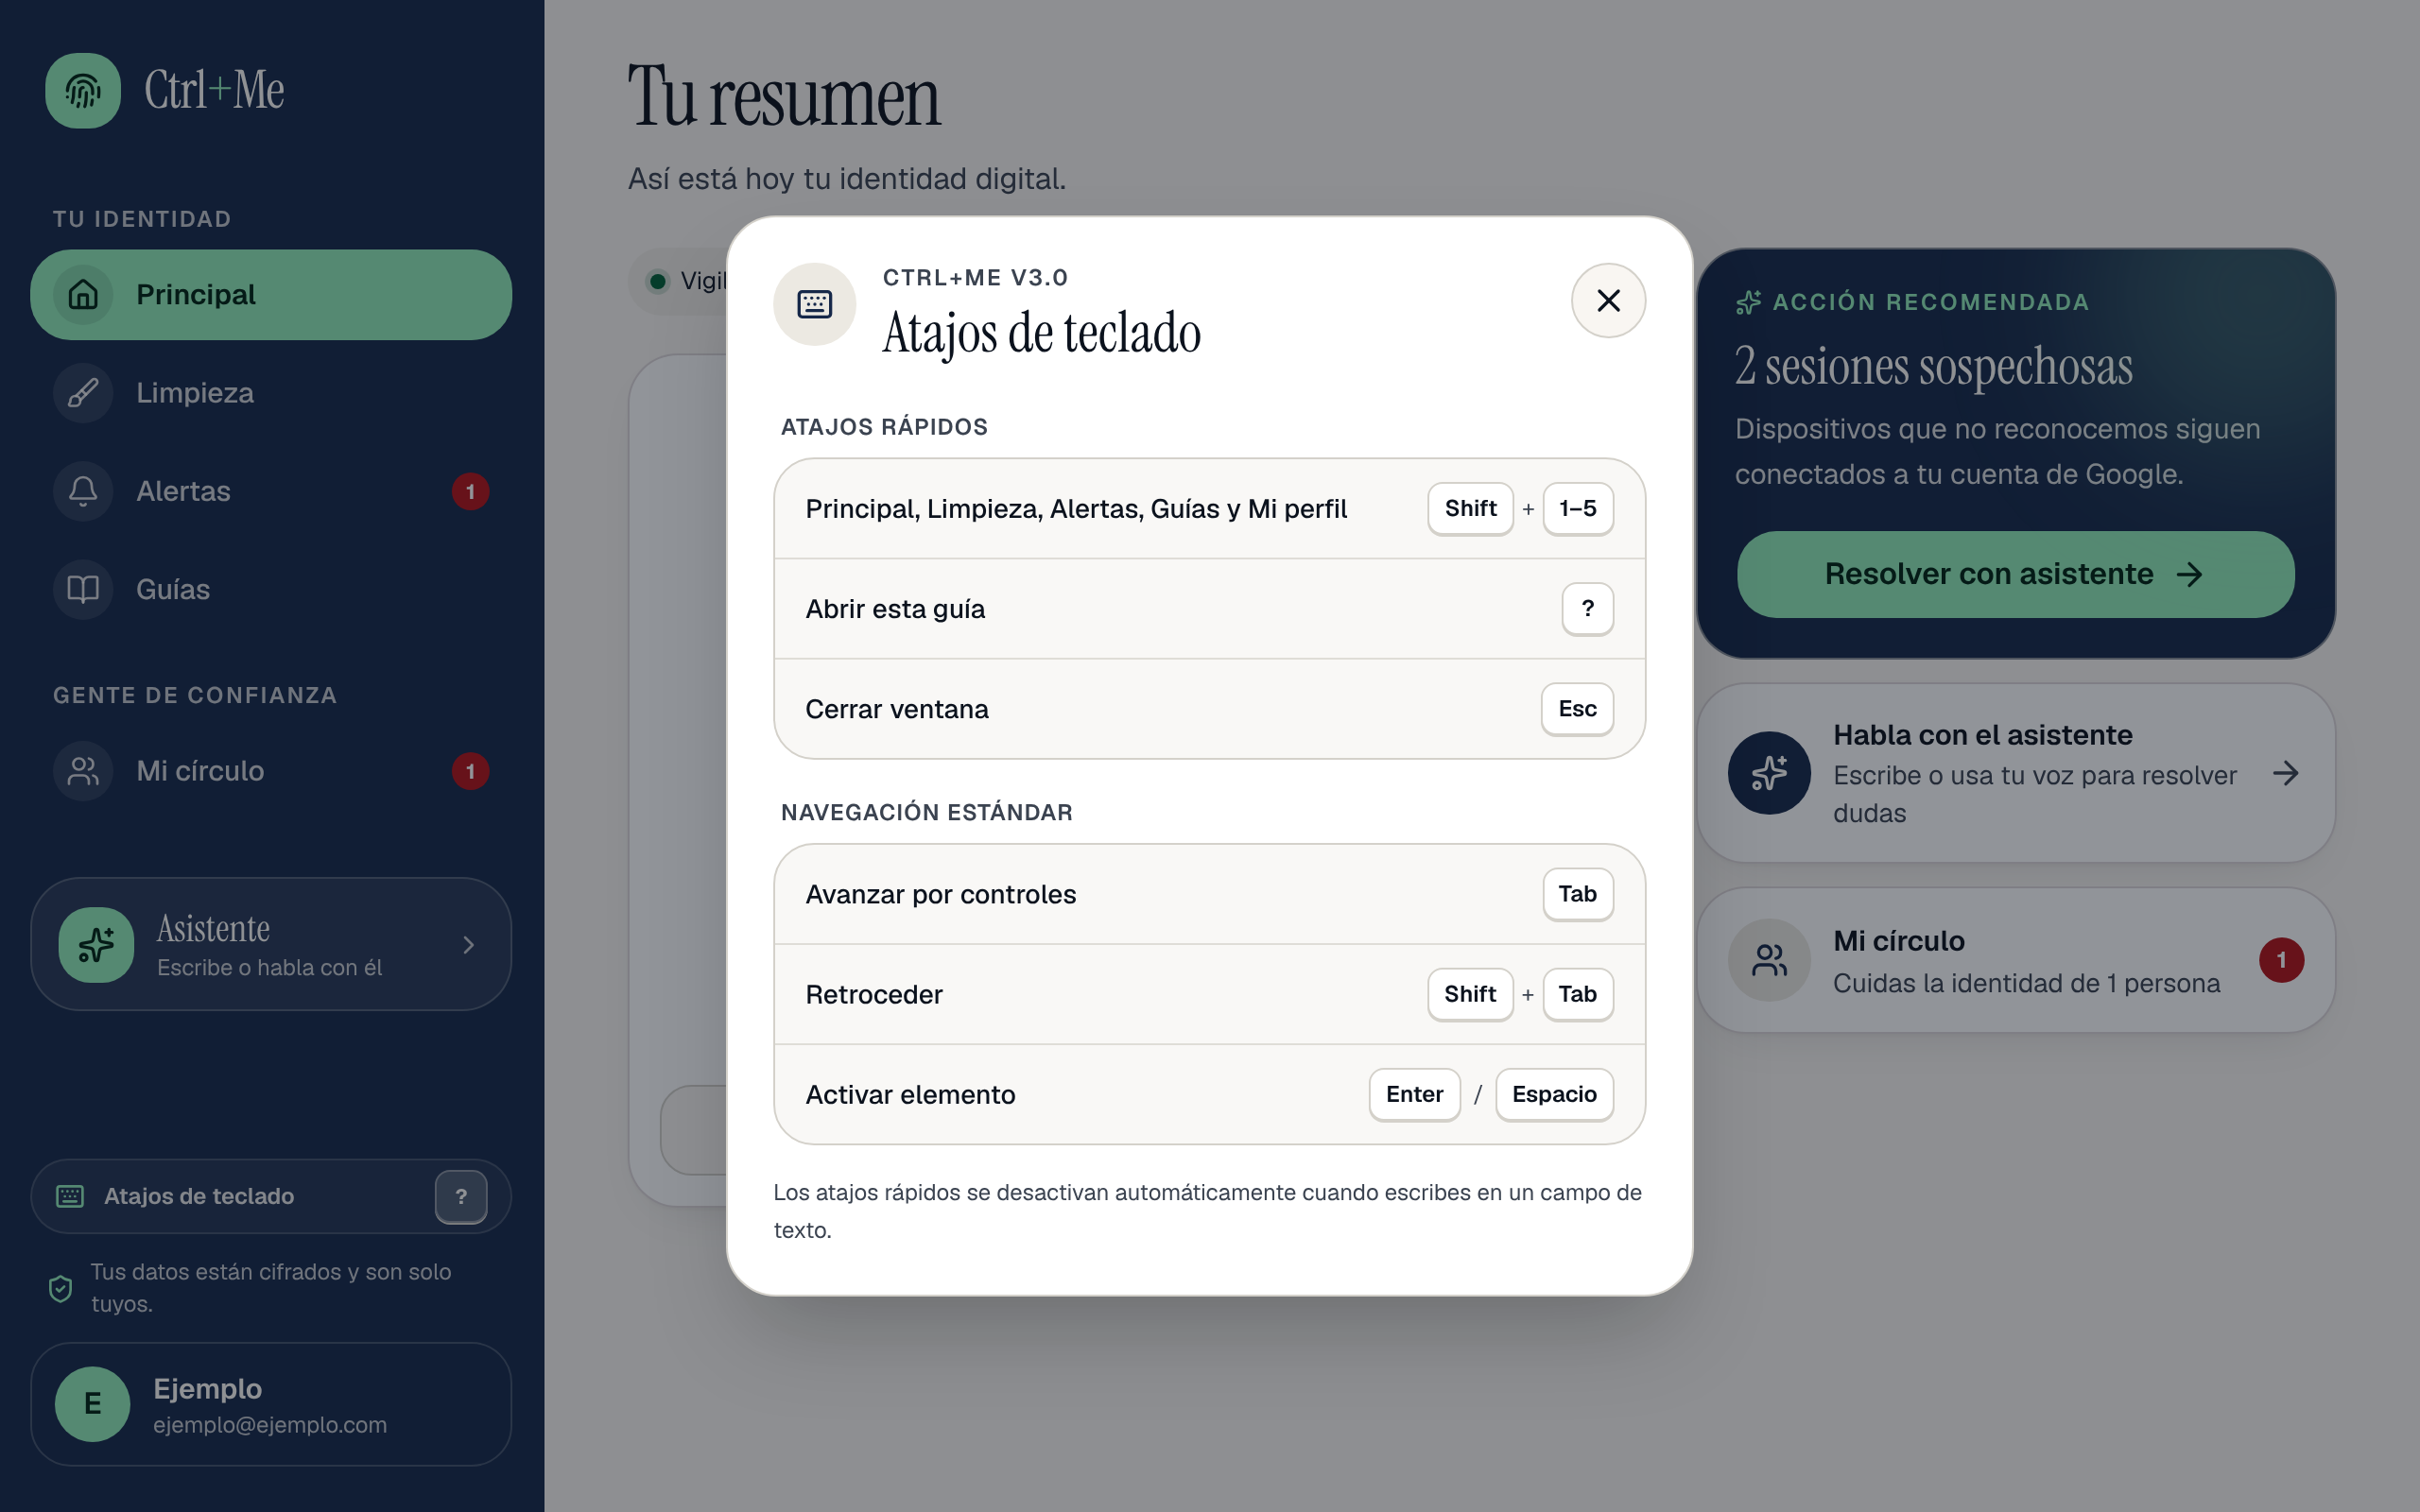
\includegraphics[width=\textwidth]{figuras-v3/v3_atajos_web.png}
    \caption{Modal de atajos de teclado (v3.0)}
    \label{fig:v3-atajos-modal}
  \end{subfigure}
  \hfill
  \begin{subfigure}[b]{0.48\textwidth}
    \centering
    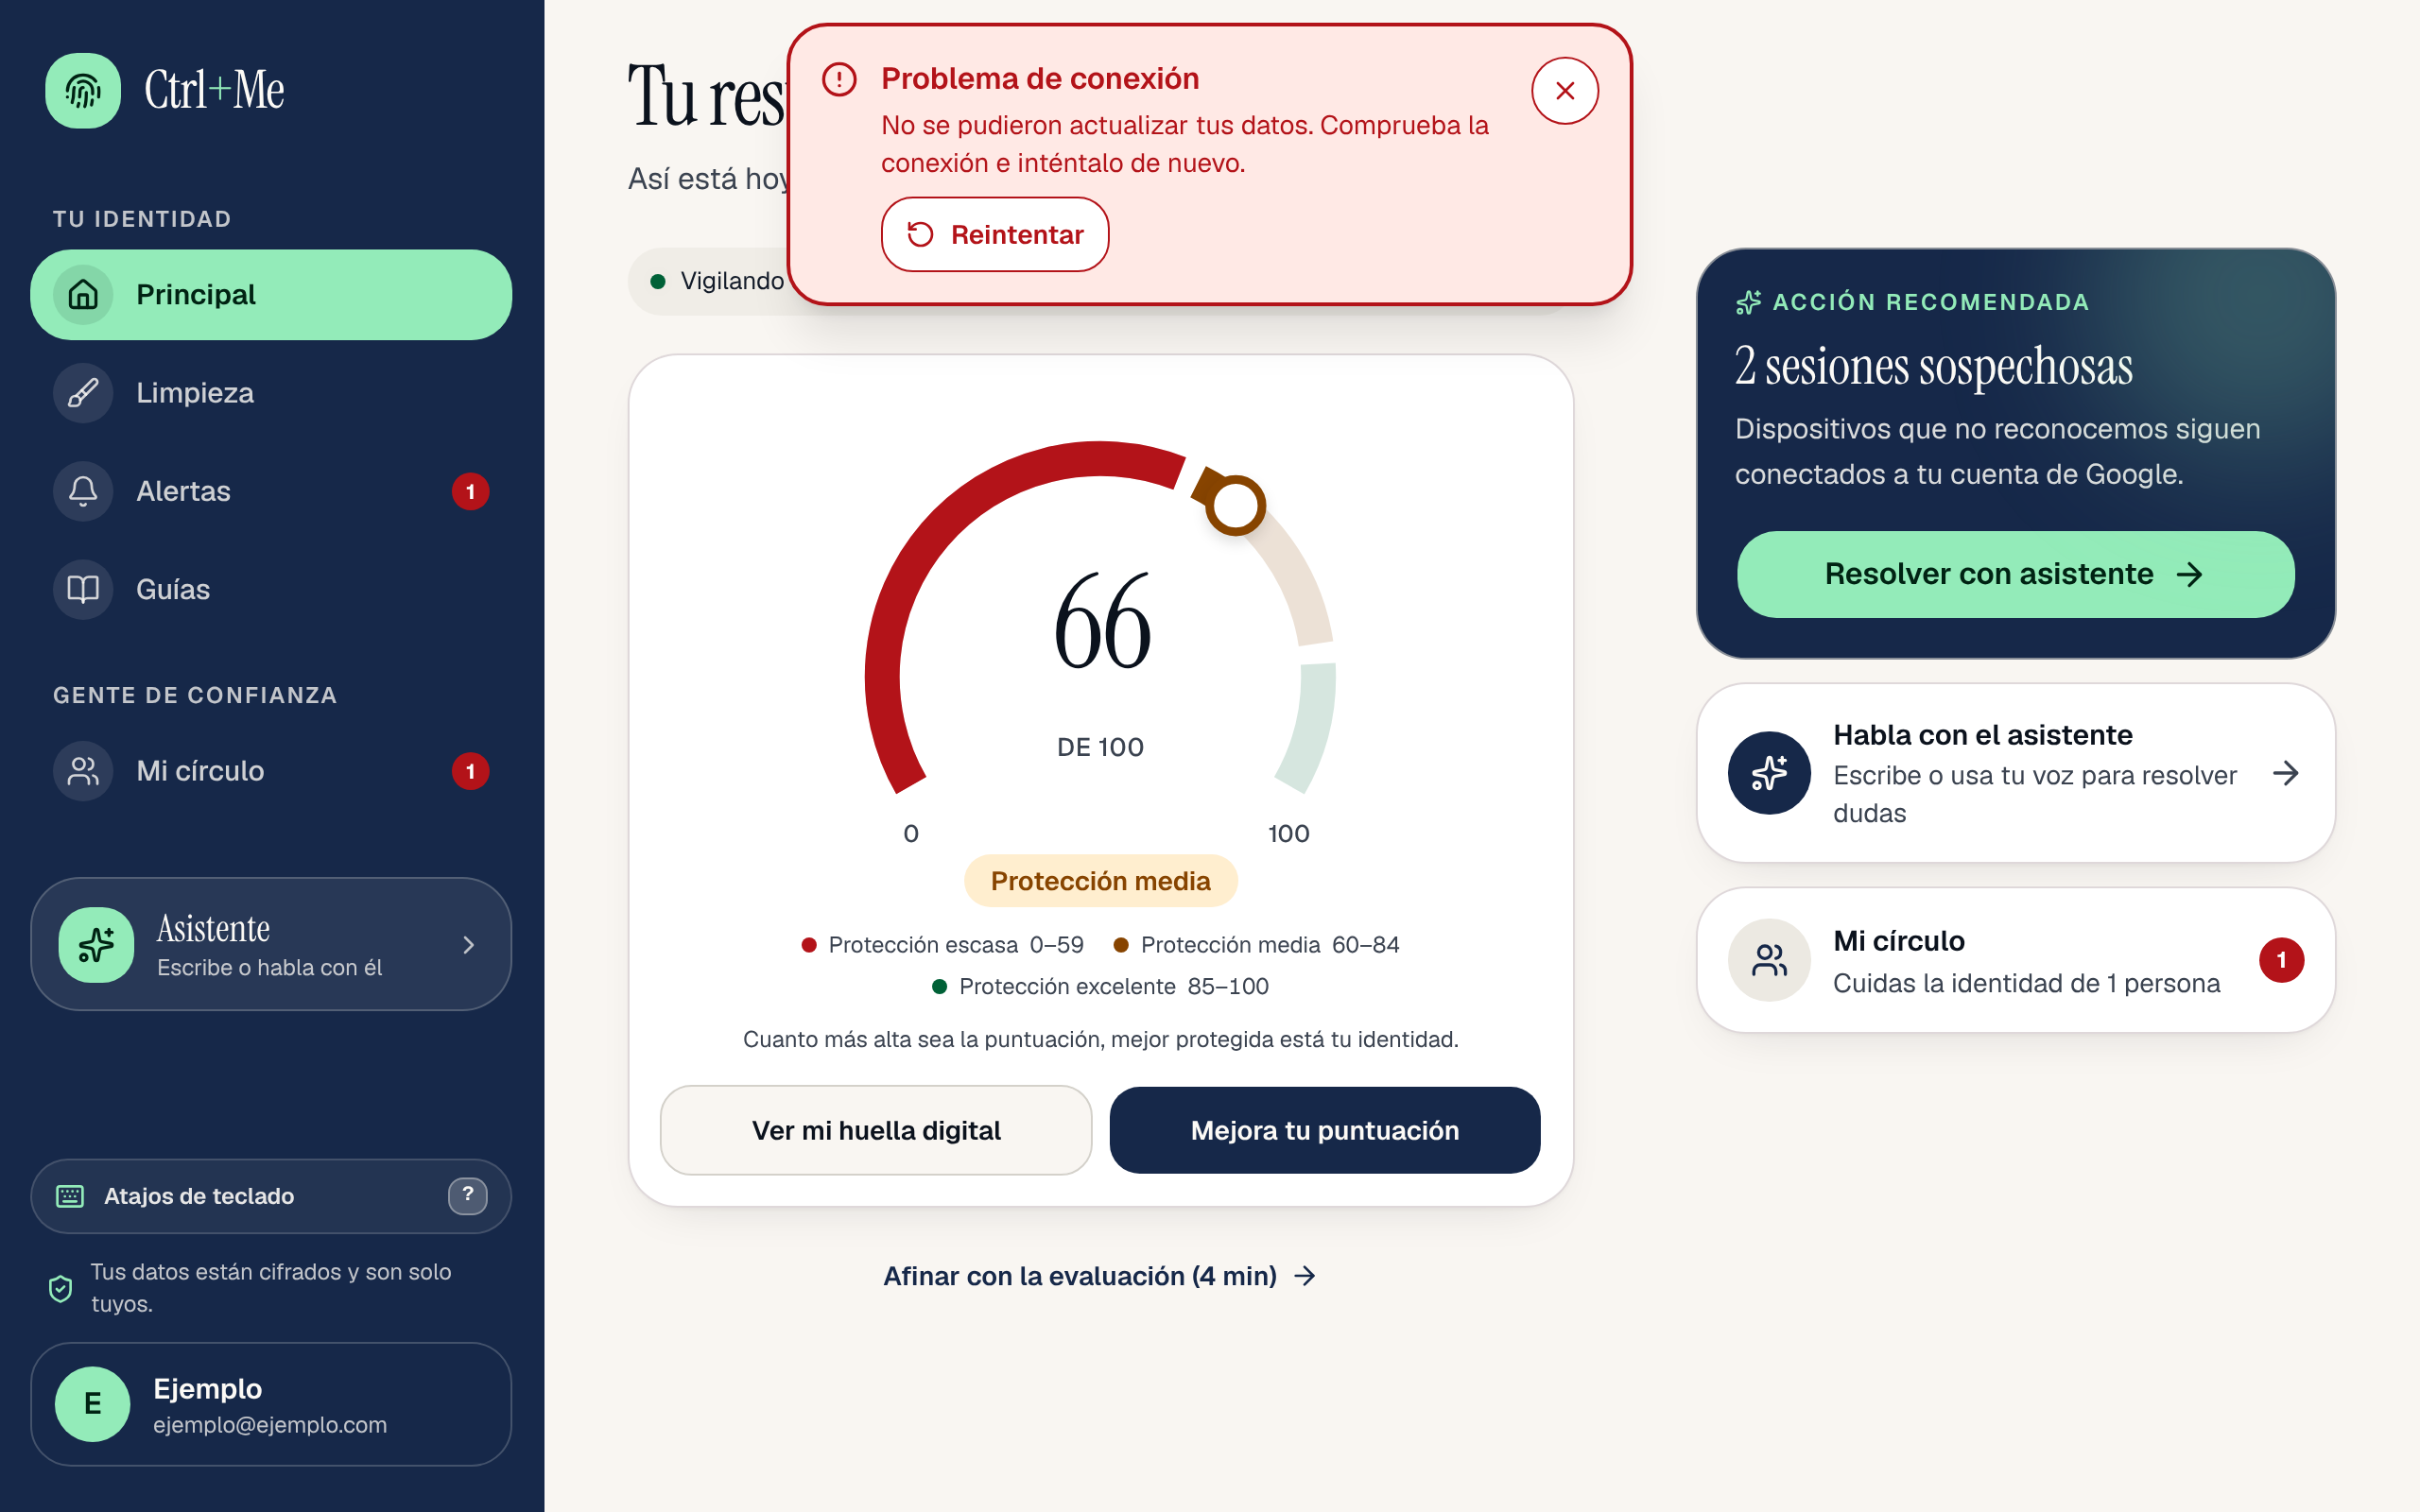
\includegraphics[width=\textwidth]{figuras-v3/v3_error_red_web.png}
    \caption{Banner de error de conexión con acción \textit{Reintentar}}
    \label{fig:v3-error-red}
  \end{subfigure}
  \caption{Guía modal de atajos de teclado globales y recuperación ante errores de red (v3.0).}
  \label{fig:v3-seguridad-atajos}
\end{figure}

\subsection{Accesibilidad personalizable: idioma, tema oscuro y alto contraste}

La sección \textbf{Accesibilidad} dentro de \textit{Mi perfil} (Figura~\ref{fig:v3-accesibilidad}) implementa de manera independiente los requisitos \textbf{R-ACC-1} y \textbf{R-ACC-3} de la Tabla~\ref{tab:requisitos-accesibilidad}, dejando visibles y accesibles los cuatro ajustes persistentes del dispositivo:

\begin{itemize}
  \item \textbf{Soporte bilingüe completo ES / EN (R-ACC-1):} Disponible en el selector compacto \textbf{ES | EN} de bienvenida y registro (sin tapar \textit{Paso X de 3}) y mediante el desplegable \textbf{Idioma / Language} en \textit{Mi perfil}, traduciendo por completo navegación, etiquetas ARIA, alertas, limpieza, cuestionario, guías y asistente (Figura~\ref{fig:v3-modos-web}).
  \item \textbf{Apariencia Claro / Oscuro, Alto contraste y Tamaño de texto (R-ACC-3):} Combinación independiente de \textit{Claro / Oscuro}, interruptor \textbf{Alto contraste} (\textit{High contrast}) y escala tipográfica (\textit{100\,\%, 125\,\%, 150\,\%}) extendida a todas las vistas de la aplicación, preservando la legibilidad de tarjetas críticas como las alertas de filtración en modo oscuro (Figura~\ref{fig:v3-alertas-oscuro-web}).
\end{itemize}

\begin{figure}[H]
  \centering
  \begin{subfigure}[b]{0.64\textwidth}
    \centering
    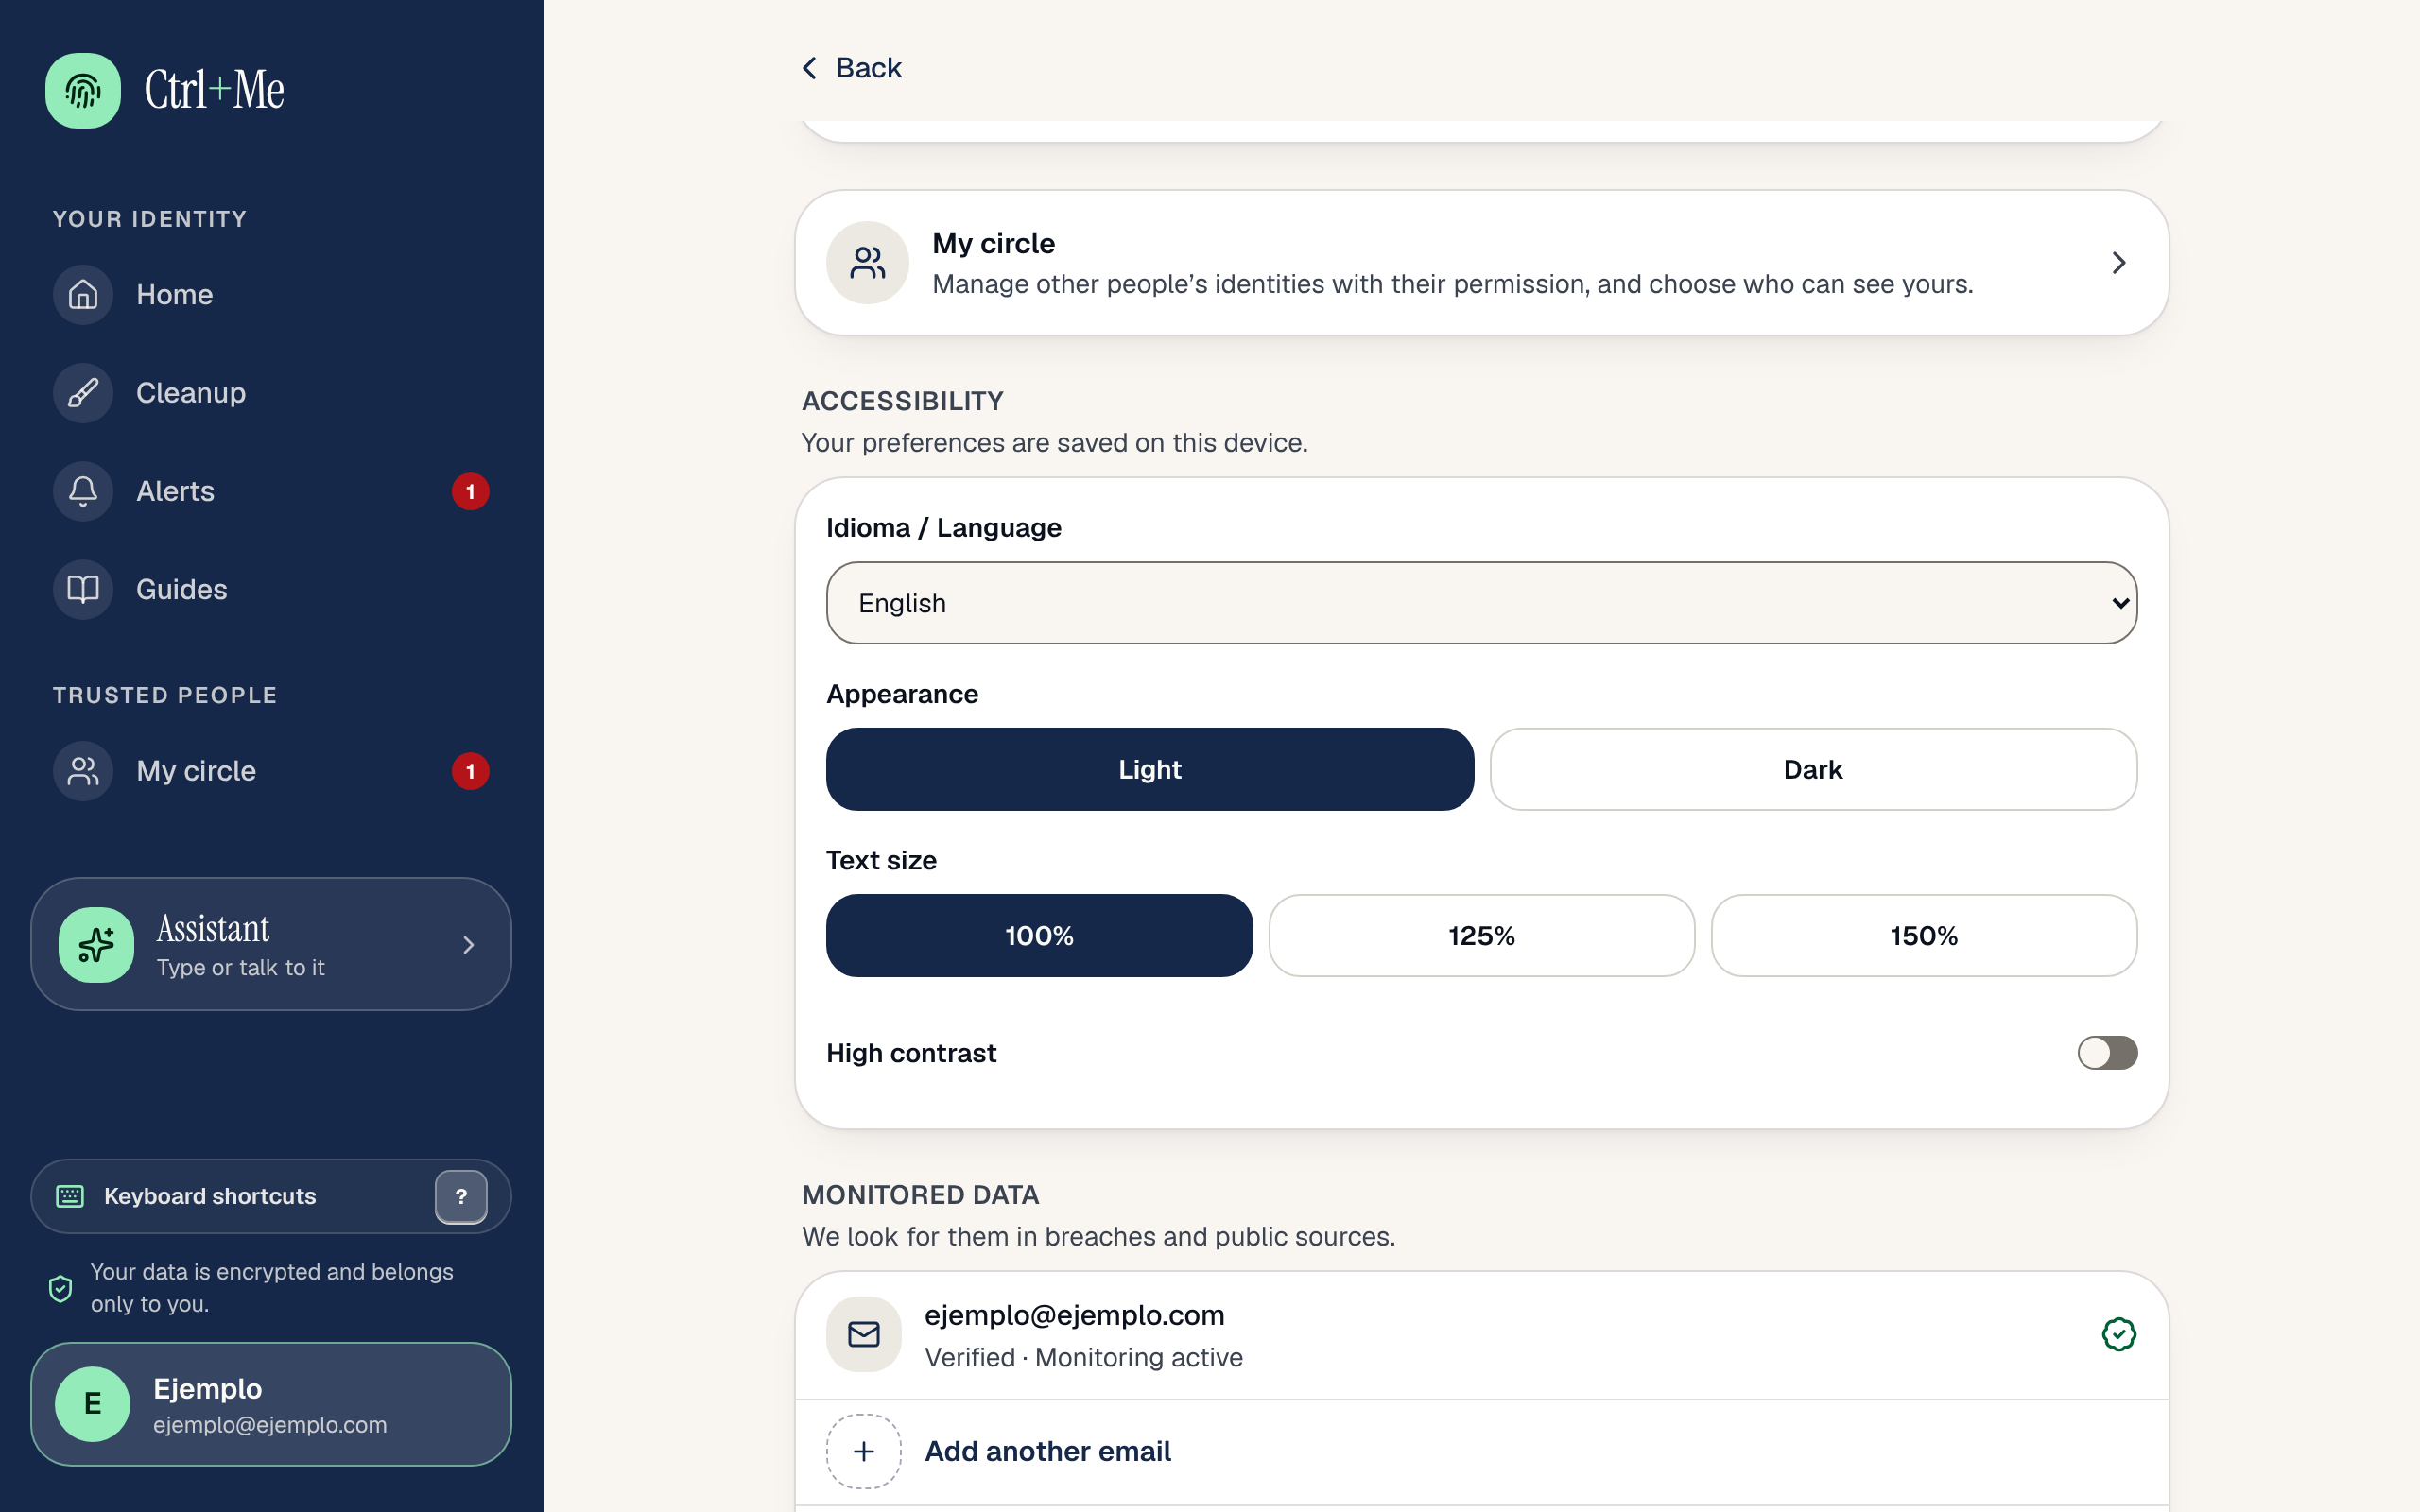
\includegraphics[width=\textwidth]{figuras-v3/v3_perfil_accesibilidad_en_web.png}
    \caption{Sección Accessibility en inglés con interruptor \textit{High contrast} (web)}
    \label{fig:v3-perfil-acc-web}
  \end{subfigure}
  \hfill
  \begin{subfigure}[b]{0.30\textwidth}
    \centering
    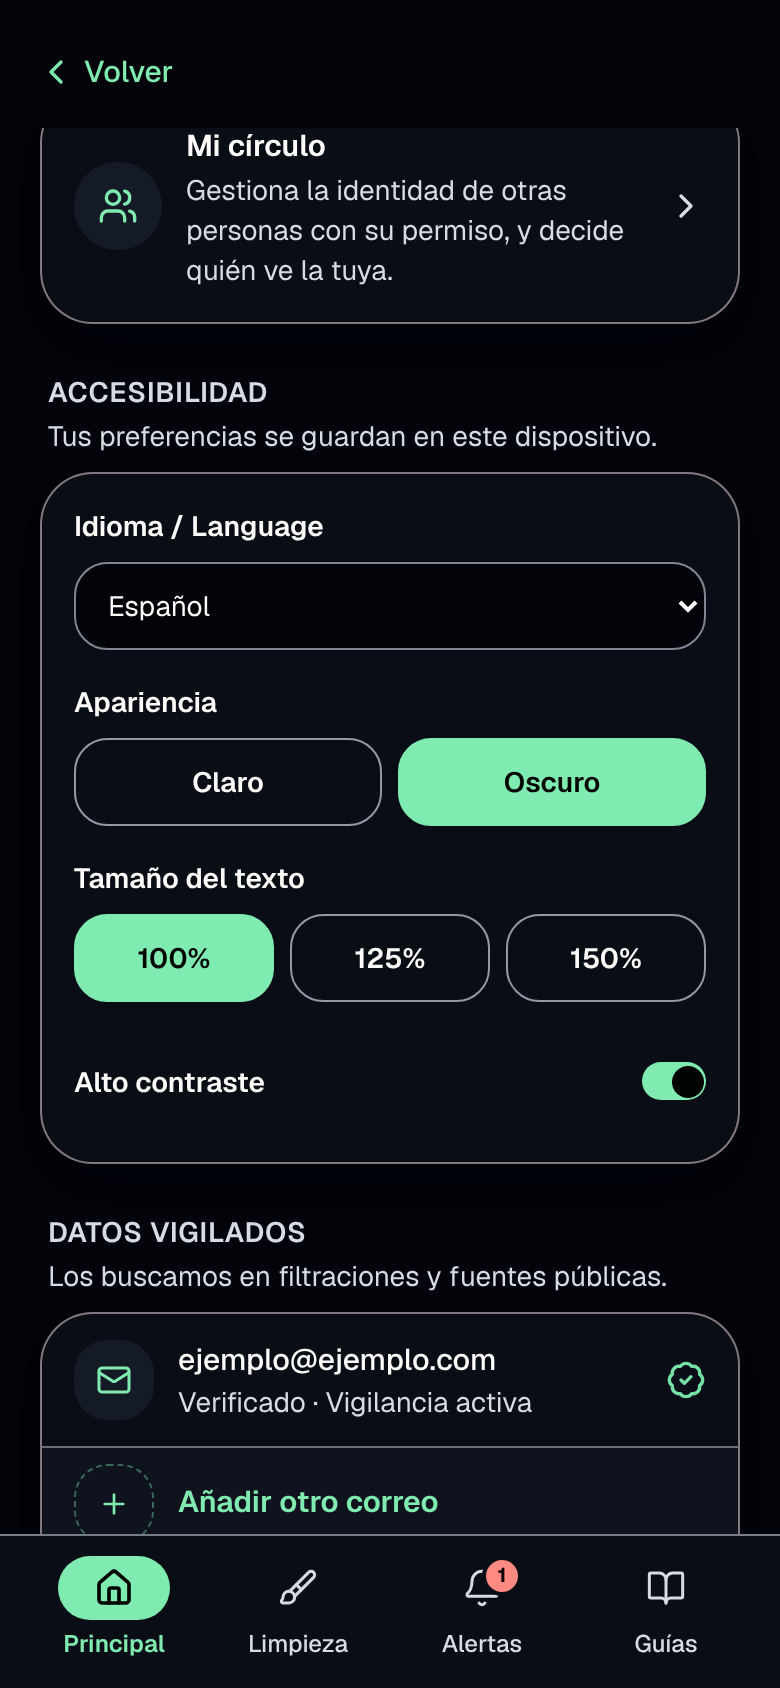
\includegraphics[width=\textwidth]{figuras-v3/v3_perfil_oscuro_alto_contraste_movil.png}
    \caption{Oscuro + Alto contraste activado (móvil)}
    \label{fig:v3-perfil-oscuro-ac-movil}
  \end{subfigure}
  \caption{Controles completos de Accesibilidad en \textit{Mi perfil}: idioma, apariencia, tamaño de texto y alto contraste.}
  \label{fig:v3-accesibilidad}
\end{figure}

\begin{figure}[H]
  \centering
  \begin{subfigure}[b]{0.48\textwidth}
    \centering
    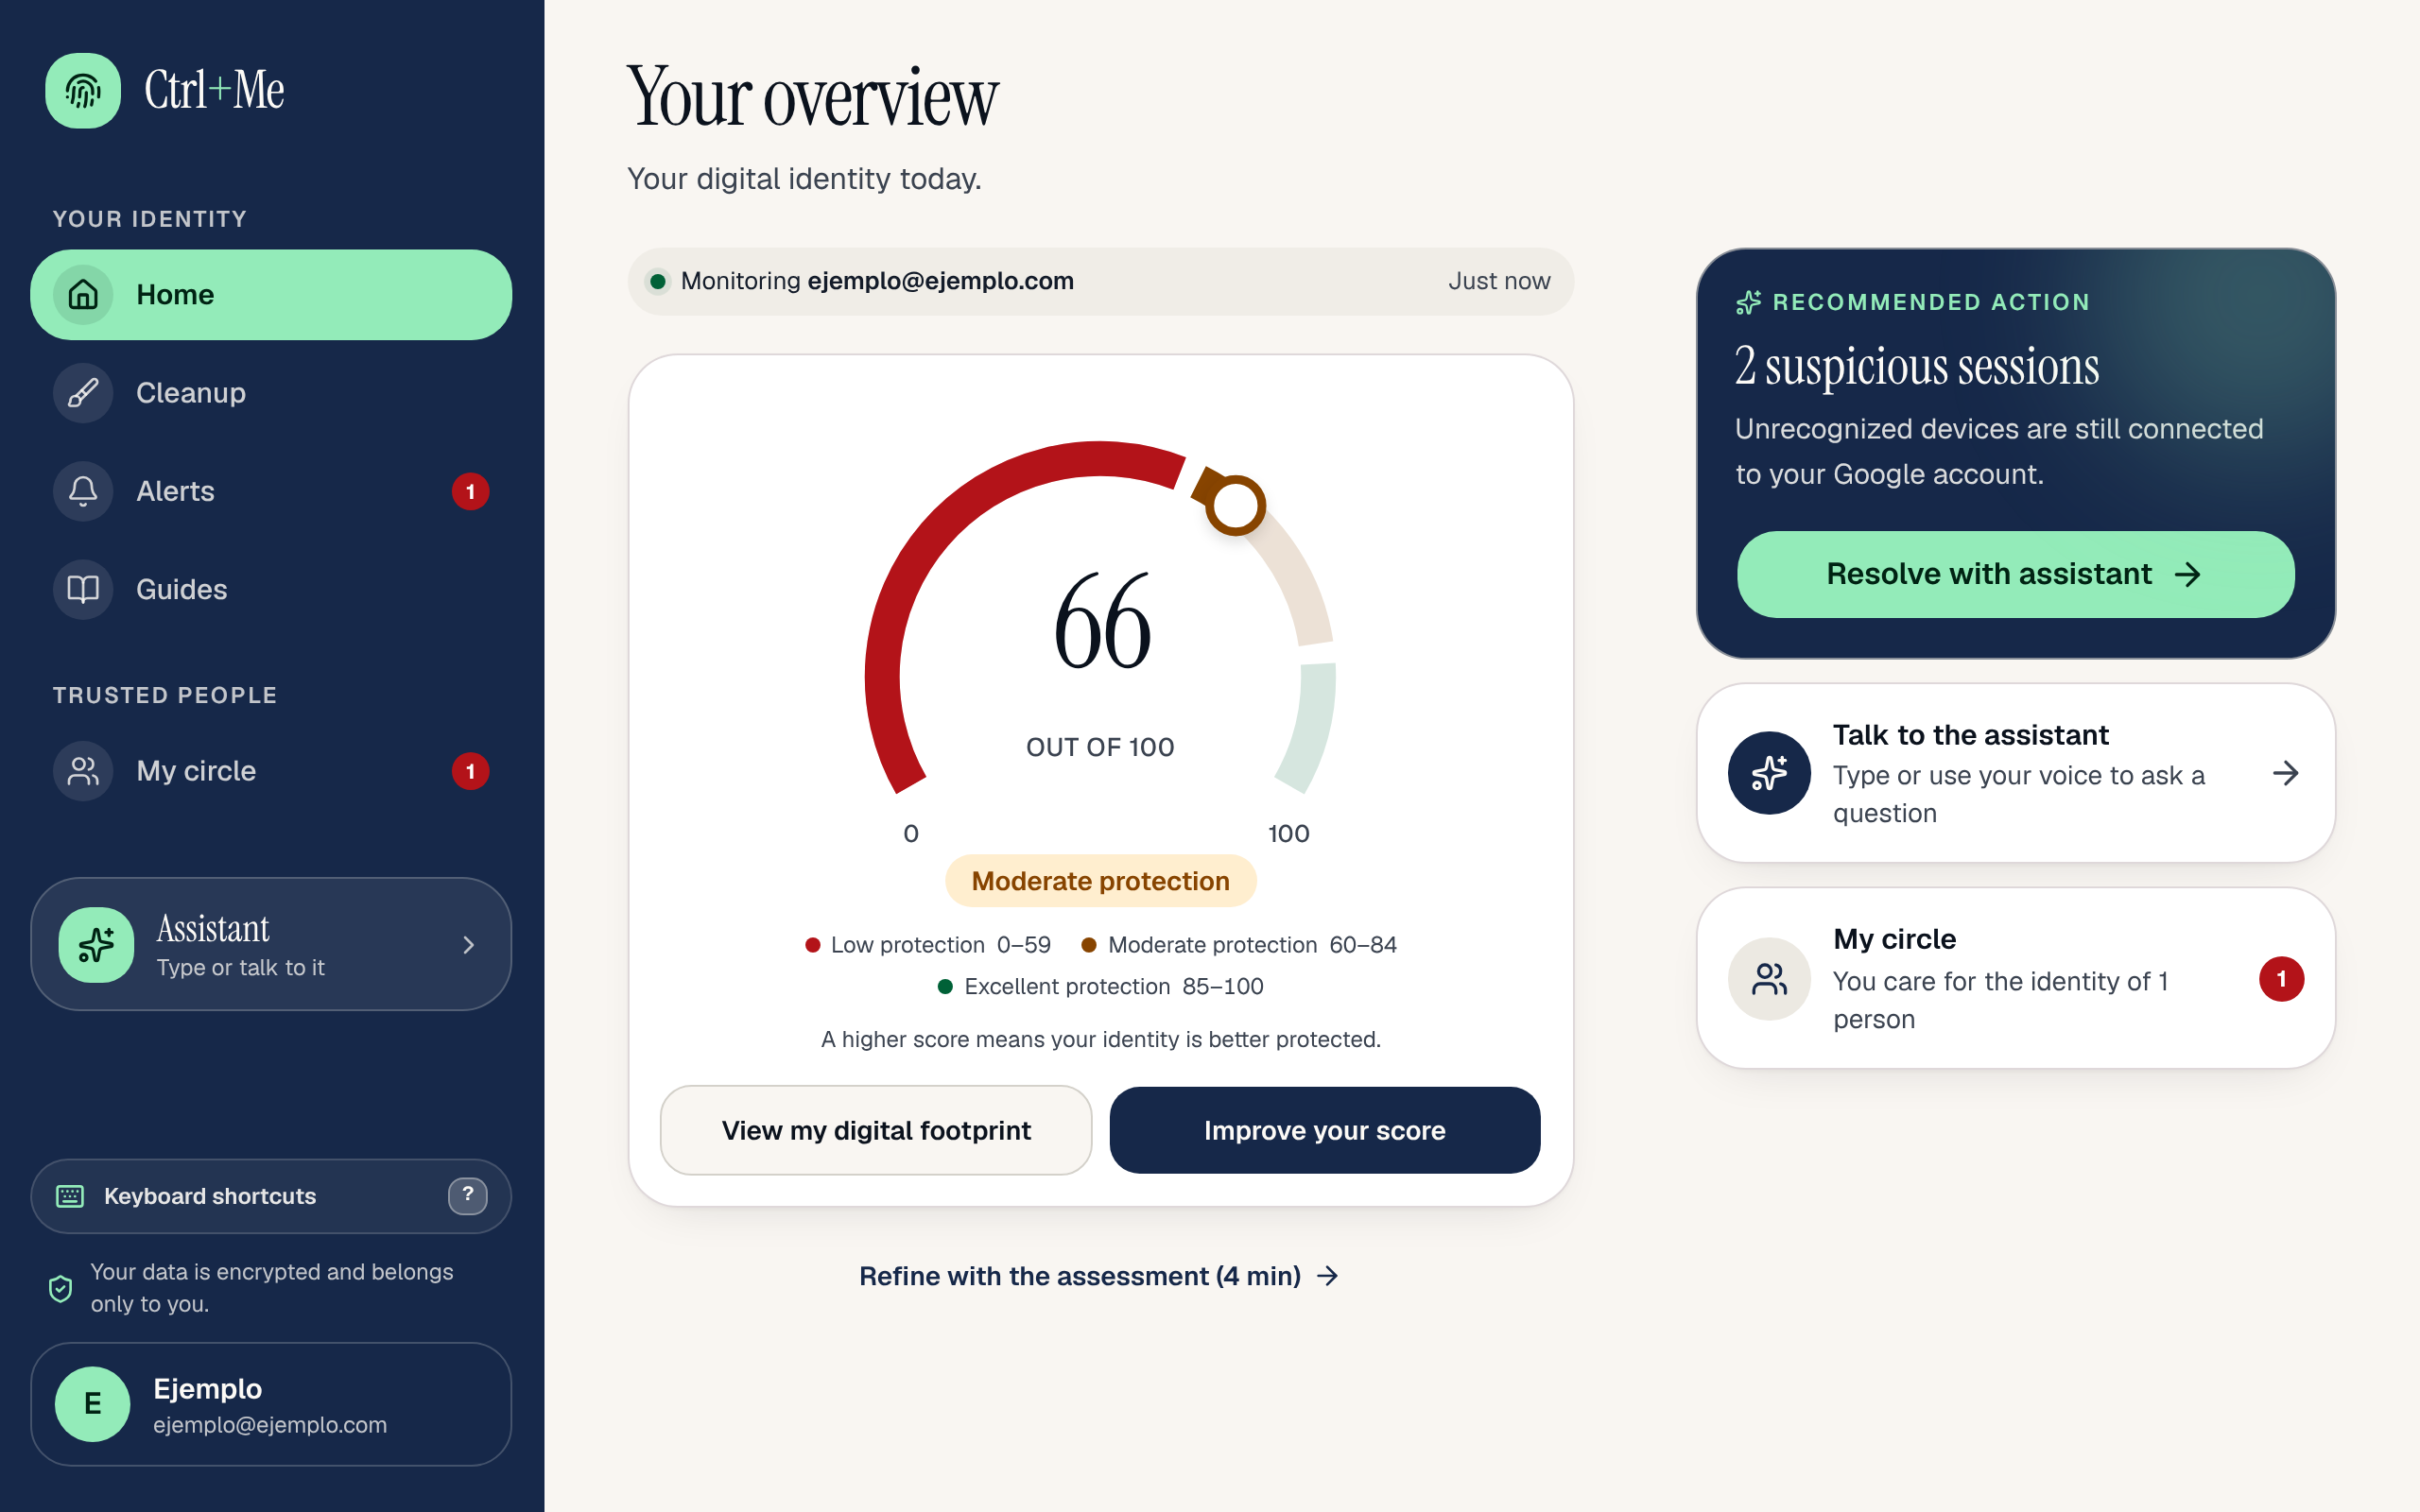
\includegraphics[width=\textwidth]{figuras-v3/v3_principal_en_web.png}
    \caption{Pantalla principal traducida al inglés (EN)}
    \label{fig:v3-principal-en}
  \end{subfigure}
  \hfill
  \begin{subfigure}[b]{0.48\textwidth}
    \centering
    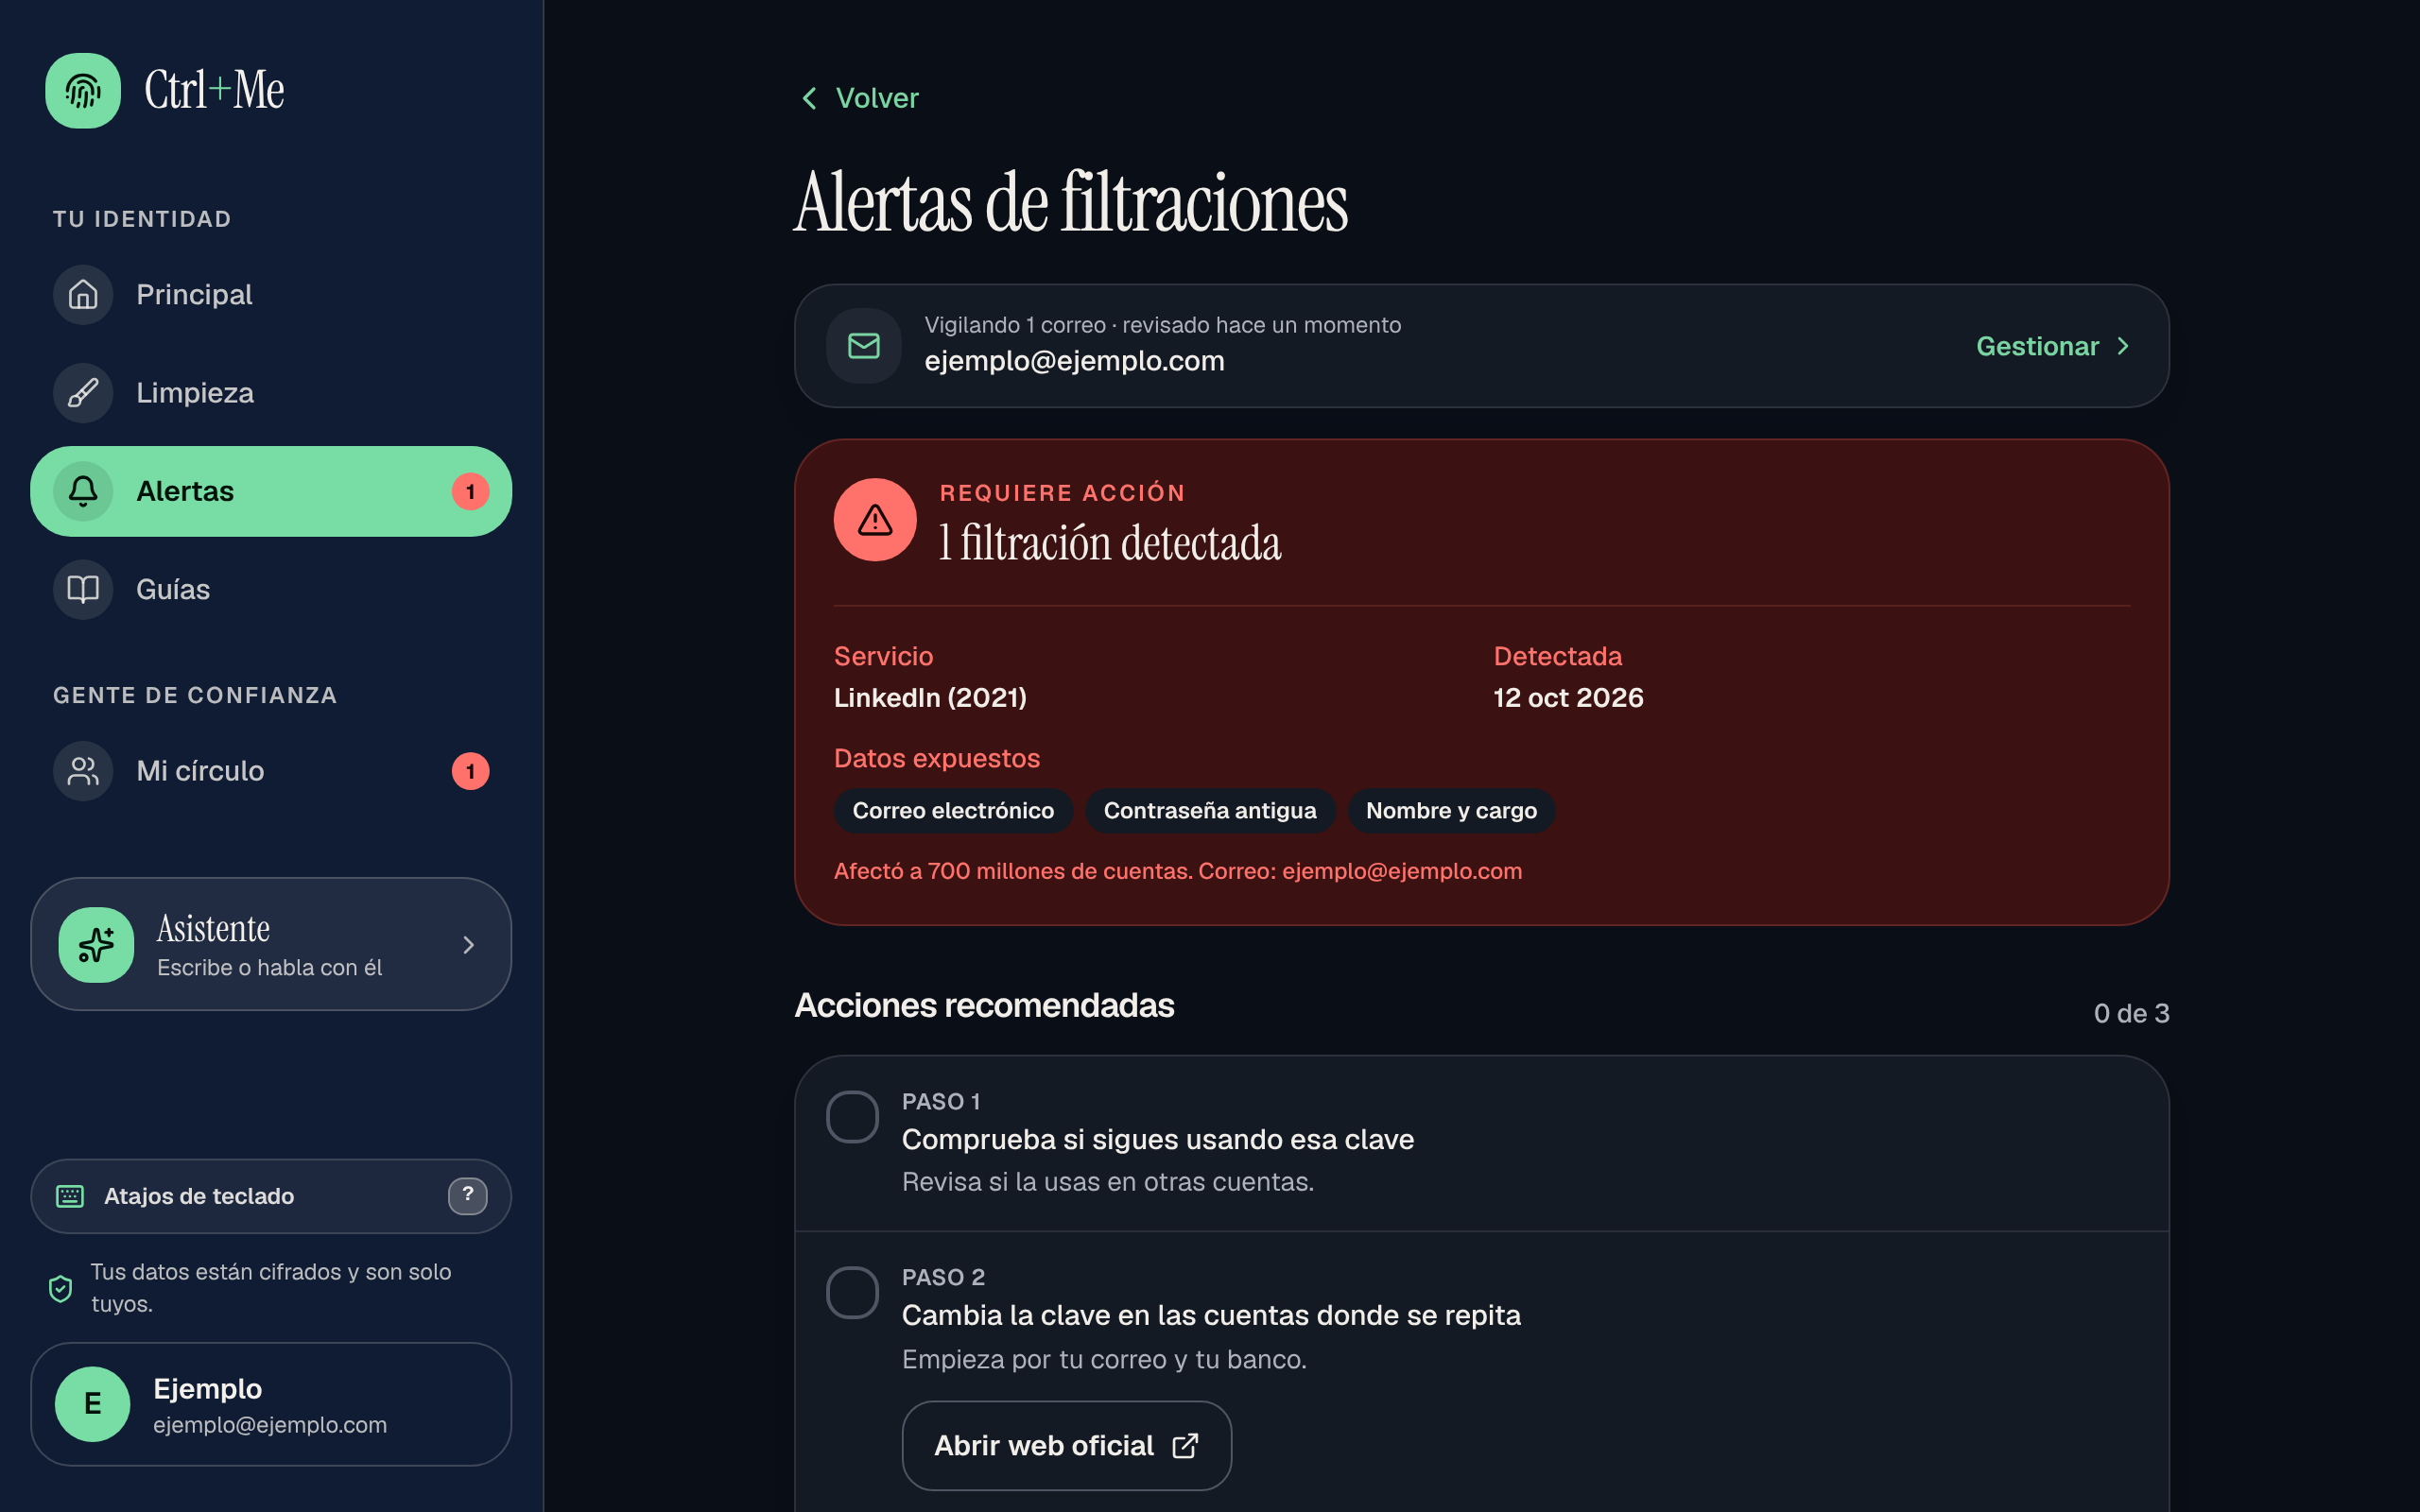
\includegraphics[width=\textwidth]{figuras-v3/v3_alertas_oscuro_web.png}
    \caption{Alertas de filtración en modo oscuro}
    \label{fig:v3-alertas-oscuro-web}
  \end{subfigure}
  \caption{Soporte bilingüe completo en inglés y modo oscuro extendido a tarjetas de alerta críticas.}
  \label{fig:v3-modos-web}
\end{figure}

\subsection{Relación entre requisitos y cambios efectuados en v3.0}

La Tabla~\ref{tab:trazabilidad-v3} resume la correspondencia directa entre los nuevos requisitos de las Tablas~\ref{tab:requisitos-usabilidad} y~\ref{tab:requisitos-accesibilidad} y los cambios implementados en Ctrl+Me v3.0.

\begin{table}[H]
  \centering
  \caption{Relación entre los requisitos de usabilidad y accesibilidad y los cambios realizados en el prototipo v3.0.}
  \label{tab:trazabilidad-v3}
  \small
  \begin{tabularx}{\textwidth}{@{}l X l@{}}
    \toprule
    \textbf{Requisito (Tabla)} & \textbf{Cambio efectuado en la interfaz v3.0} & \textbf{Evidencia} \\
    \midrule
    R-USA-1 (Tabla~\ref{tab:requisitos-usabilidad}) & Renombrado del arco y leyenda a \textit{Protección escasa / media / excelente} frente a \textit{Exposición baja / media / alta}. & Fig.~\ref{fig:v3-principal} \\
    R-USA-2 (Tabla~\ref{tab:requisitos-usabilidad}) & Unificación de \textit{Mejora tu puntuación} en enlaces, menú y cabecera; \textit{Guías} como \texttt{h1} y \textit{Aprende en 1 minuto} como subtítulo. & Fig.~\ref{fig:v3-plan-guias} \\
    R-USA-3 (Tabla~\ref{tab:requisitos-usabilidad}) & Eliminación de tarjetas redundantes en Principal e integración de \textit{Mejora tu puntuación} junto a \textit{Ver mi huella digital}. & Fig.~\ref{fig:v3-principal} \\
    R-USA-4 (Tabla~\ref{tab:requisitos-usabilidad}) & Filtros \textit{Todas / Pendientes / Completadas} y selector de ordenación por impacto en puntos. & Fig.~\ref{fig:v3-plan-web} \\
    R-USA-5 (Tabla~\ref{tab:requisitos-usabilidad}) & Atajos \texttt{Shift+1..5}, \texttt{?}, \texttt{Esc} (pausados en campos de entrada) y diálogo renovado de \textit{Atajos de teclado}. & Fig.~\ref{fig:v3-atajos-modal} \\
    R-USA-6 (Tabla~\ref{tab:requisitos-usabilidad}) & Diálogos modales \texttt{alertdialog} antes de \textit{Borrar mis datos y cuenta} y \textit{Retirar su acceso}. & Fig.~\ref{fig:v3-anexo-4} \\
    R-USA-7 (Tabla~\ref{tab:requisitos-usabilidad}) & Foco automático ante errores en registro, alerta inline con código \texttt{000000} y banner superior de error de red. & Figs.~\ref{fig:v3-errores-autoguardado}, \ref{fig:v3-error-red} \\
    R-USA-8 (Tabla~\ref{tab:requisitos-usabilidad}) & Indicador continuo \textit{Guardado automático} con icono en todos los pasos de evaluación. & Figs.~\ref{fig:v3-evaluacion-ac-web}, \ref{fig:v3-anexo-2} \\
    \midrule
    R-ACC-1 (Tabla~\ref{tab:requisitos-accesibilidad}) & Traducción íntegra ES/EN mediante selector en bienvenida/registro y desplegable en \textit{Accesibilidad}. & Figs.~\ref{fig:v3-accesibilidad}, \ref{fig:v3-modos-web}, \ref{fig:v3-anexo-1} \\
    R-ACC-2 (Tabla~\ref{tab:requisitos-accesibilidad}) & Oscurecimiento de textos secundarios (\texttt{--muted-foreground}) en marcas temporales, ayudas y opciones. & Figs.~\ref{fig:v3-principal}, \ref{fig:v3-evaluacion-ac-web} \\
    R-ACC-3 (Tabla~\ref{tab:requisitos-accesibilidad}) & Controles independientes de tamaño (\textit{100\,\%, 125\,\%, 150\,\%}), tema (\textit{Claro / Oscuro}) y \textit{Alto contraste} en toda la aplicación. & Figs.~\ref{fig:v3-principal}, \ref{fig:v3-accesibilidad}, \ref{fig:v3-anexo-3} \\
    Validadores (CCA / WAVE) & Contraste en botones de cierre \texttt{X}, alertas rojas en oscuro, botones de limpieza, píldoras y \texttt{<header>} en Principal. & Figs.~\ref{fig:v3-plan-guias}, \ref{fig:v3-modos-web}, \ref{fig:v3-anexo-2} \\
    \bottomrule
  \end{tabularx}
\end{table}

% ============================================================================
% Anexo completo de pantallas v3.0 (sin redundancias web/móvil)
% ============================================================================
\newpage
\section{Anexo: Pantallas completas del prototipo v3.0}
\label{sec:anexo-v3}

En este anexo se recoge el resto de pantallas, flujos y combinaciones de idioma y tema que completan la cobertura del prototipo \textbf{Ctrl+Me v3.0}, combinando capturas web y móviles representativas de cada vista para evitar duplicidades innecesarias.

\begin{figure}[H]
  \centering
  \begin{subfigure}[b]{0.27\textwidth}
    \centering
    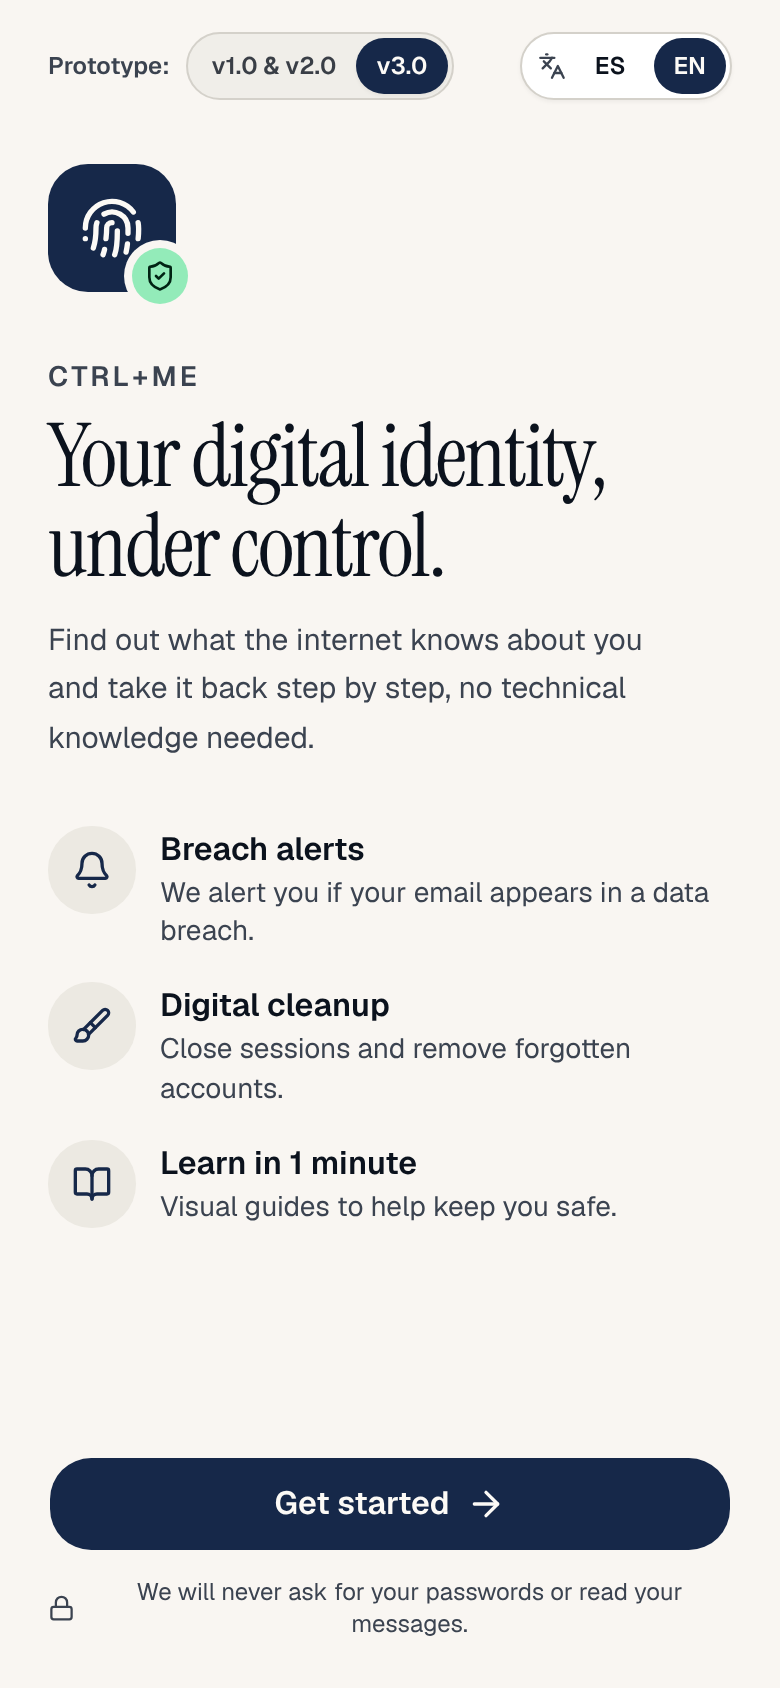
\includegraphics[width=\textwidth]{figuras-v3/v3_bienvenida_en_movil.png}
    \caption{Bienvenida en inglés con selector ES | EN (móvil)}
  \end{subfigure}
  \hfill
  \begin{subfigure}[b]{0.27\textwidth}
    \centering
    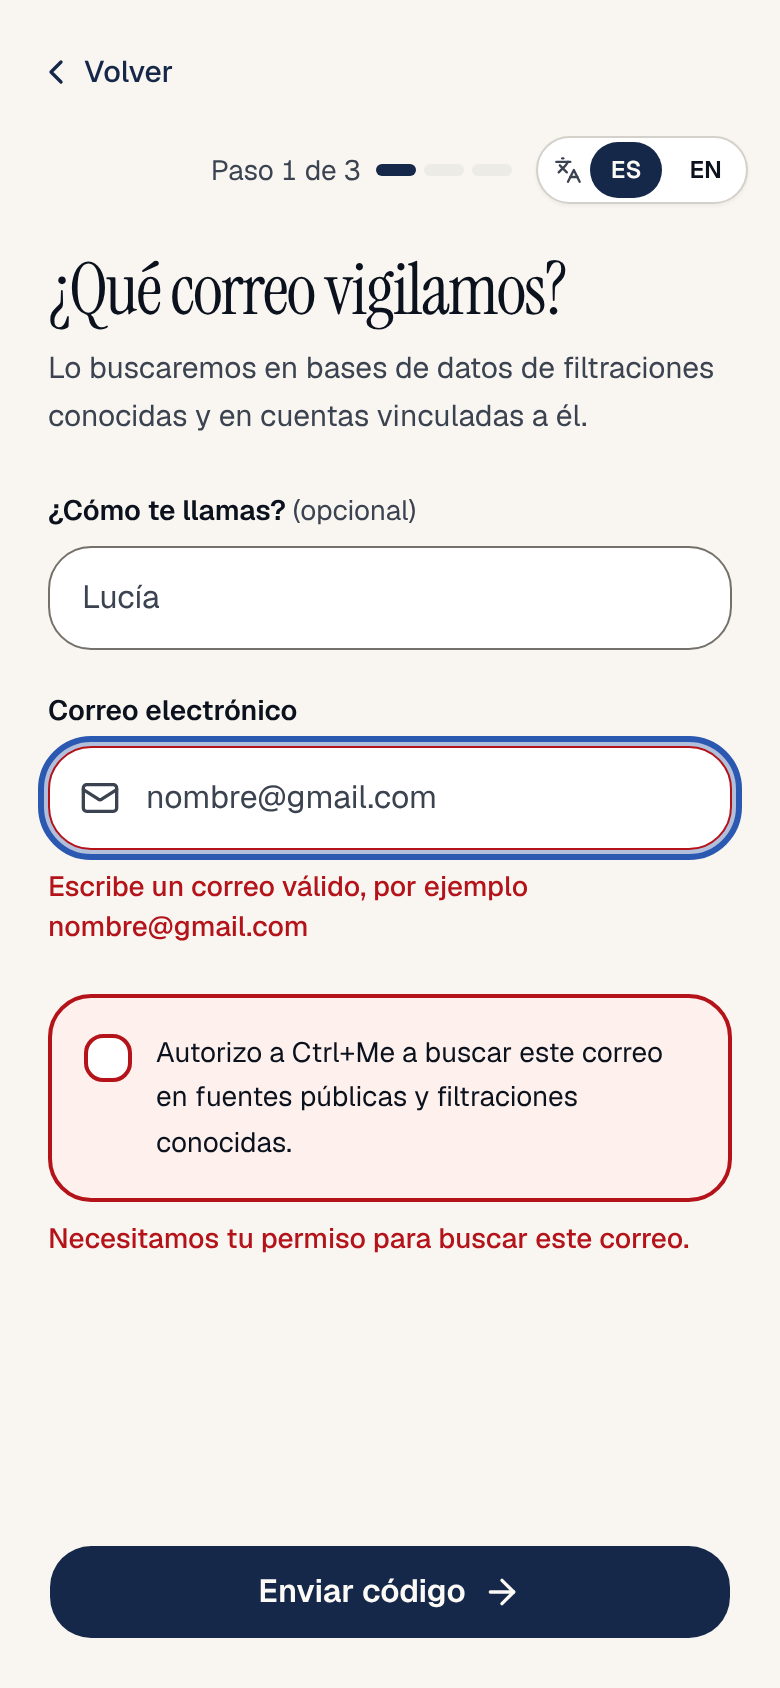
\includegraphics[width=\textwidth]{figuras-v3/v3_onboarding_error_foco_movil.png}
    \caption{Foco automático en error de correo (Paso 1, móvil)}
  \end{subfigure}
  \hfill
  \begin{subfigure}[b]{0.42\textwidth}
    \centering
    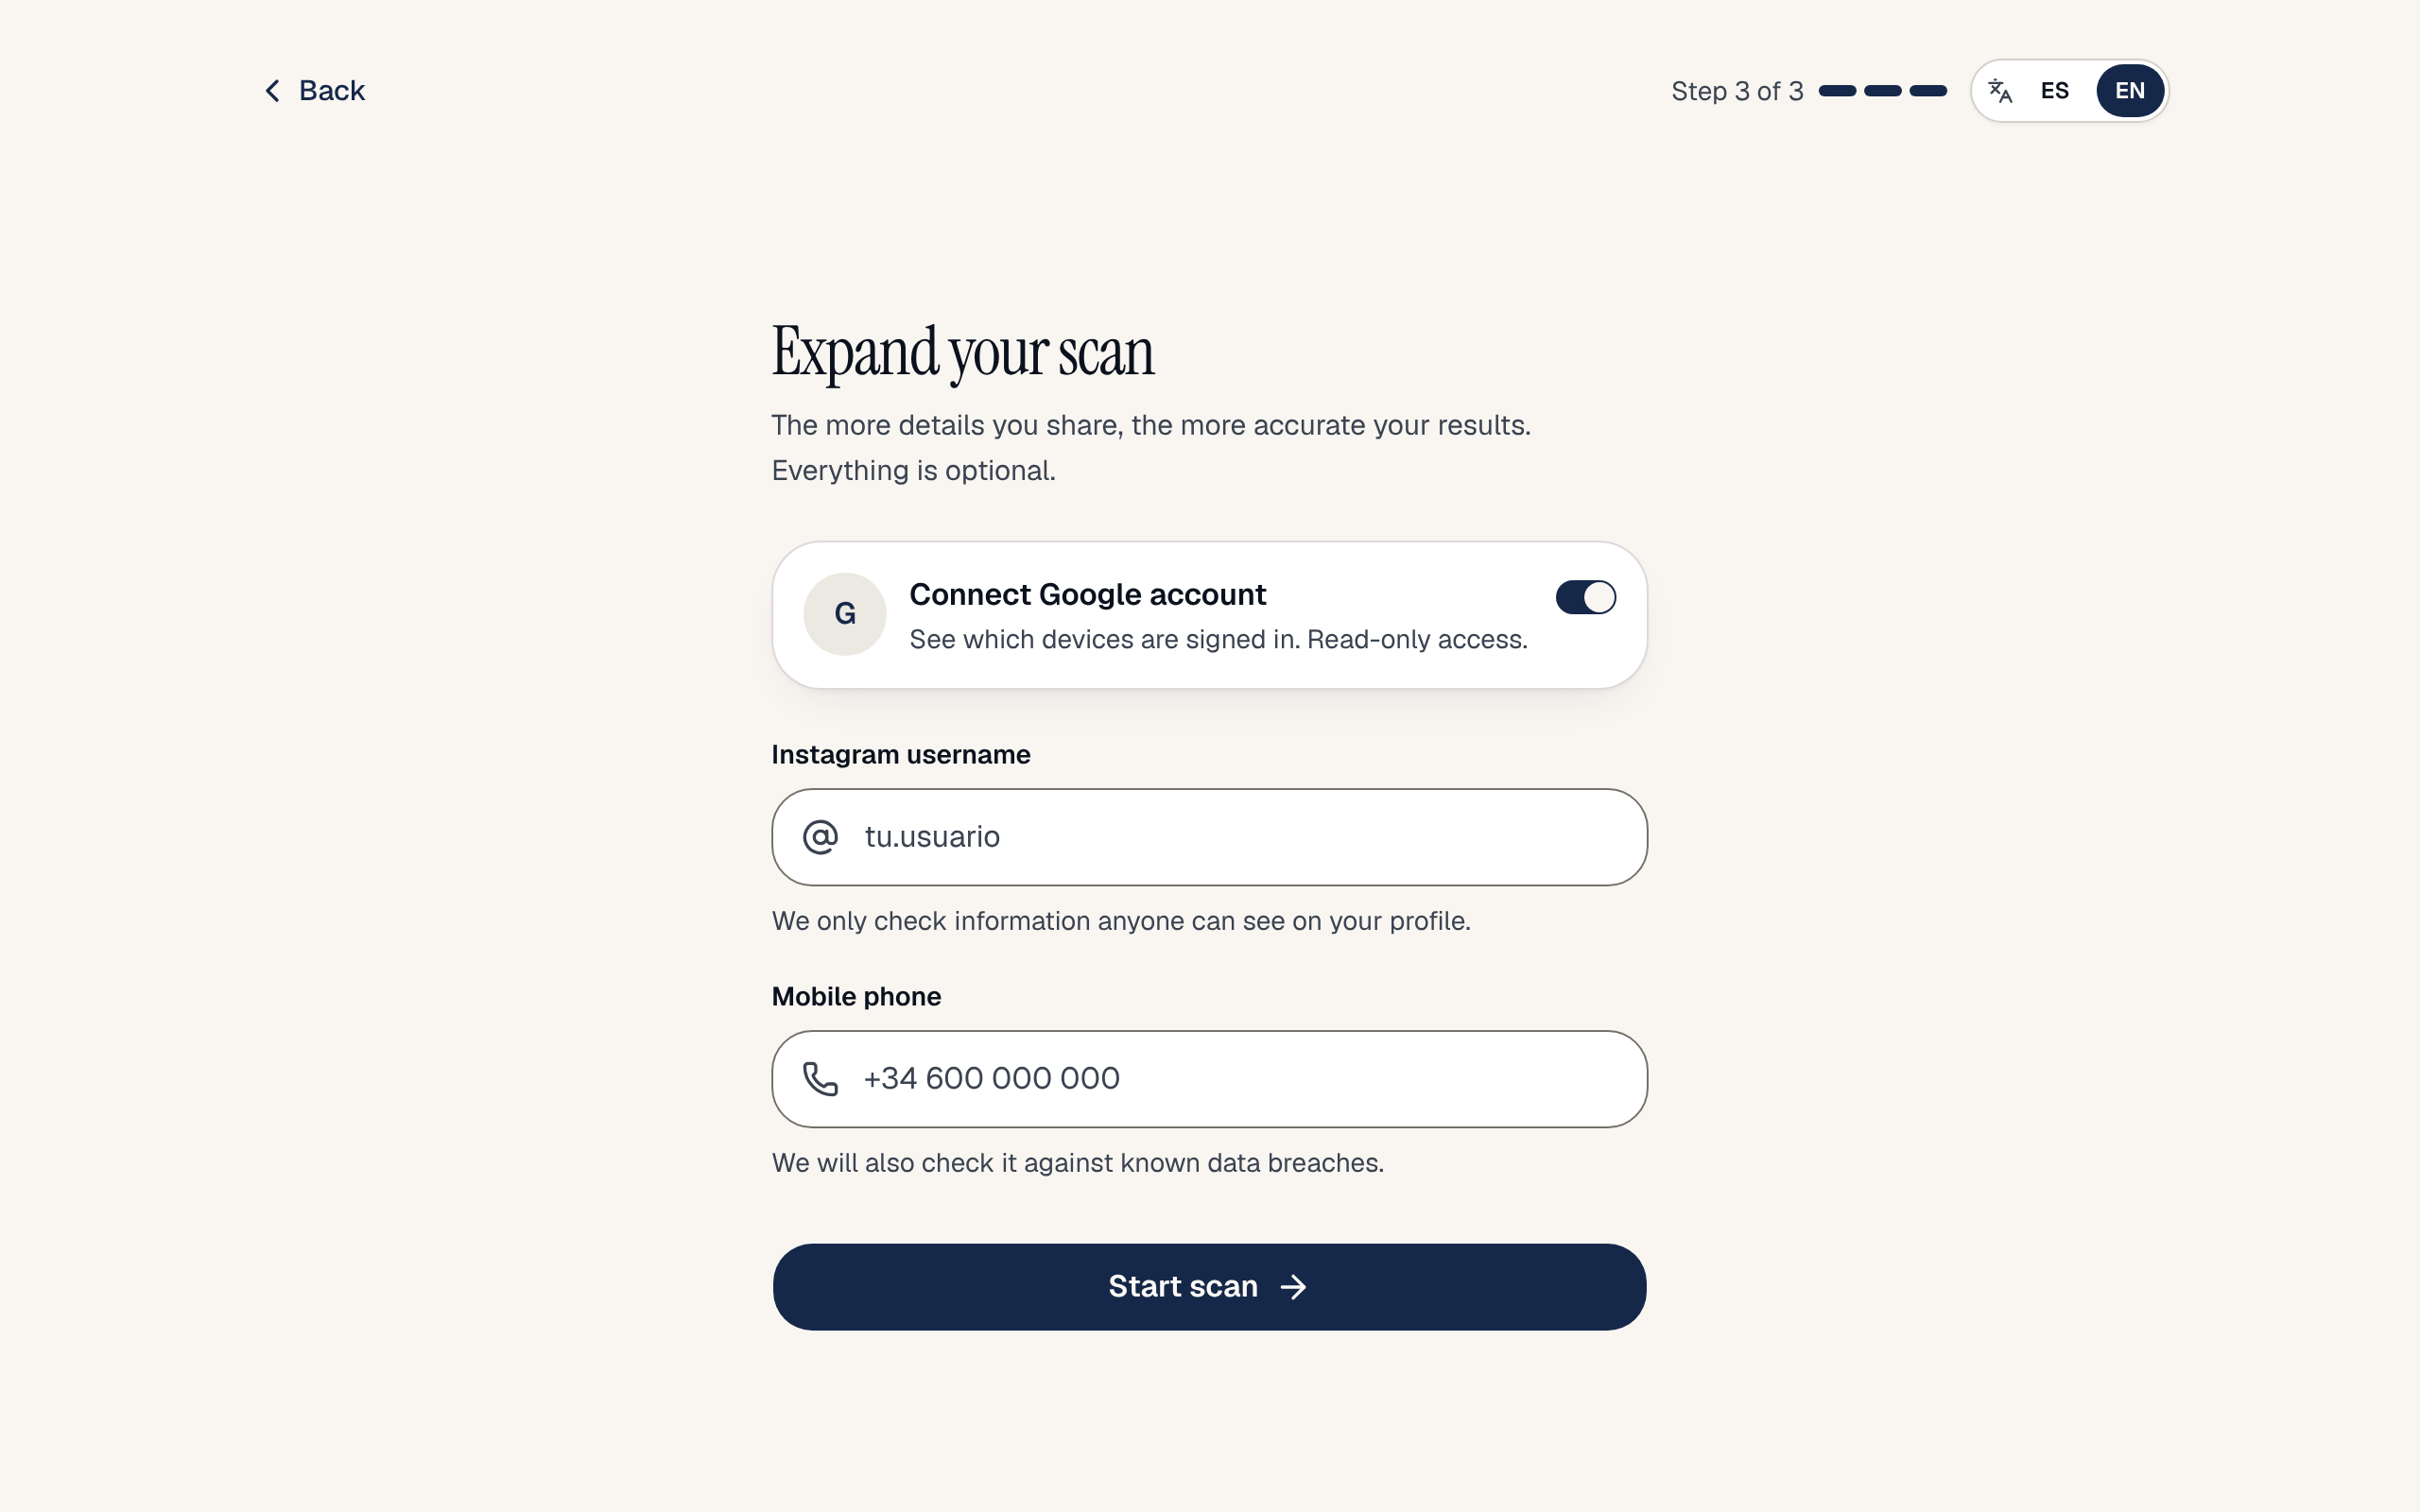
\includegraphics[width=\textwidth]{figuras-v3/v3_onboarding_conectar_en_web.png}
    \caption{Ampliación del análisis en inglés (Paso 3, web)}
  \end{subfigure}
  \\[0.75em]
  \begin{subfigure}[b]{0.48\textwidth}
    \centering
    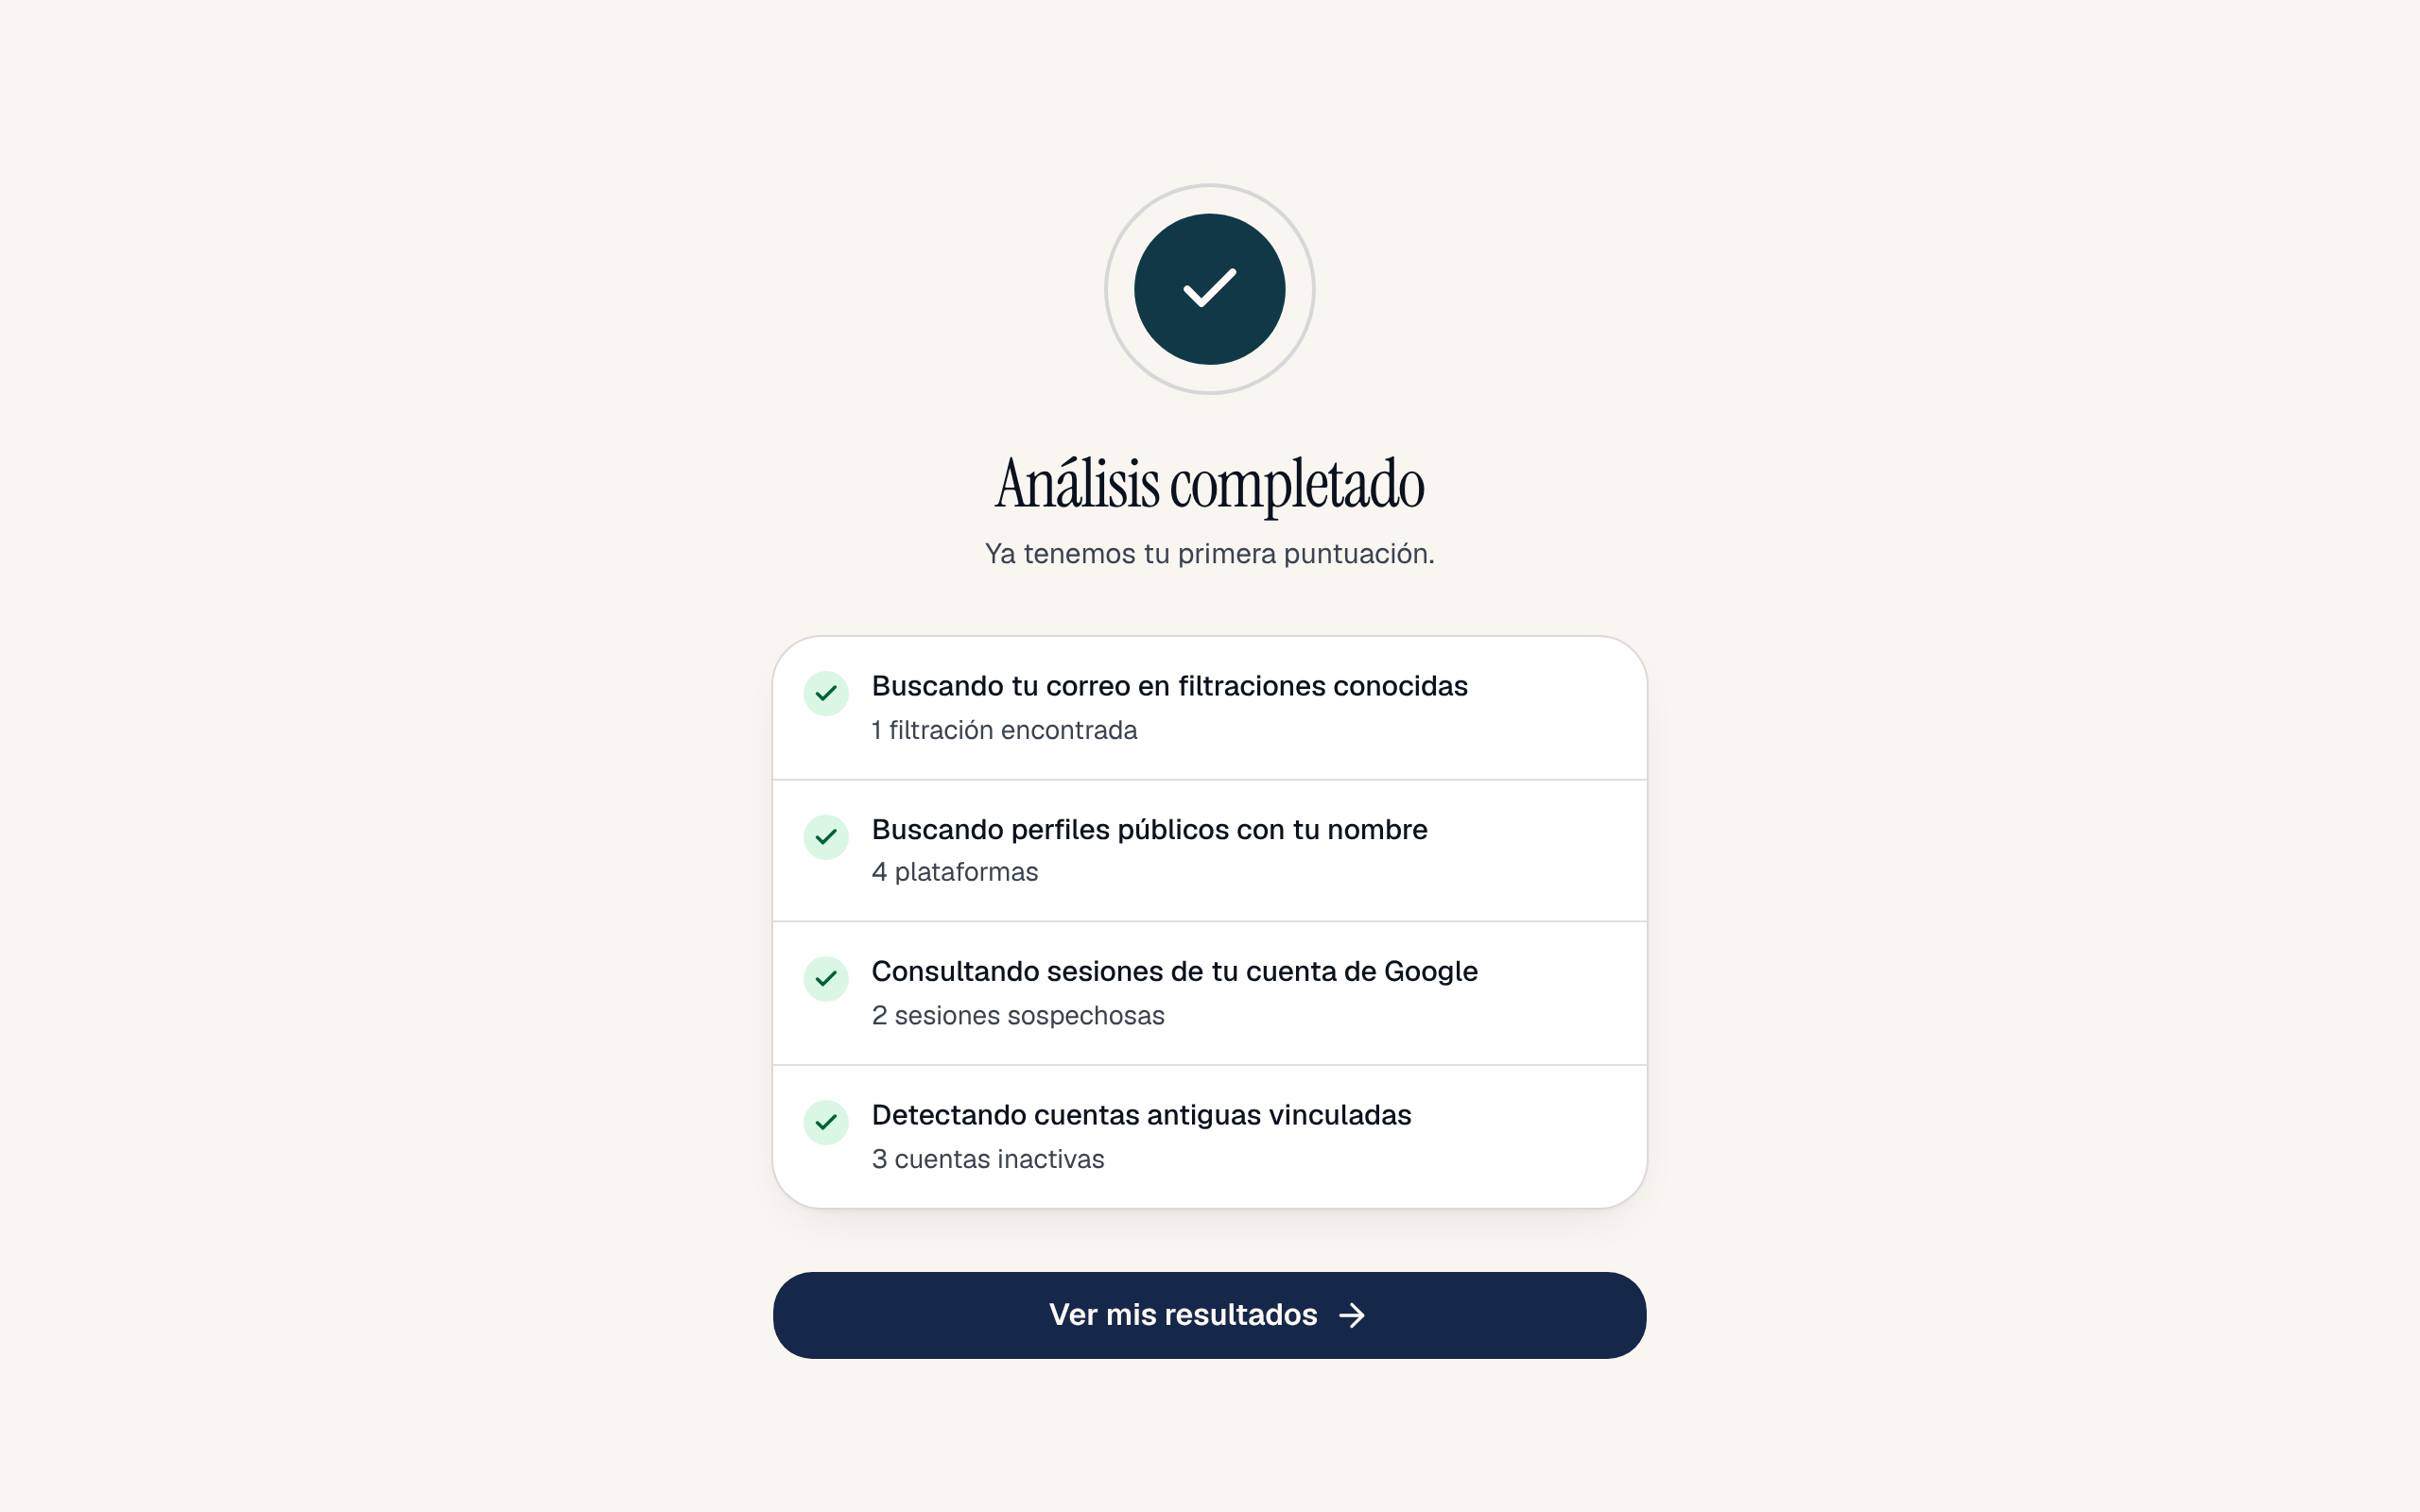
\includegraphics[width=\textwidth]{figuras-v3/v3_analisis_web.png}
    \caption{Análisis inicial completado (web)}
  \end{subfigure}
  \caption{Pantallas complementarias de bienvenida bilingüe, foco de validación en registro y análisis inicial (v3.0).}
  \label{fig:v3-anexo-1}
\end{figure}

\begin{figure}[H]
  \centering
  \begin{subfigure}[b]{0.48\textwidth}
    \centering
    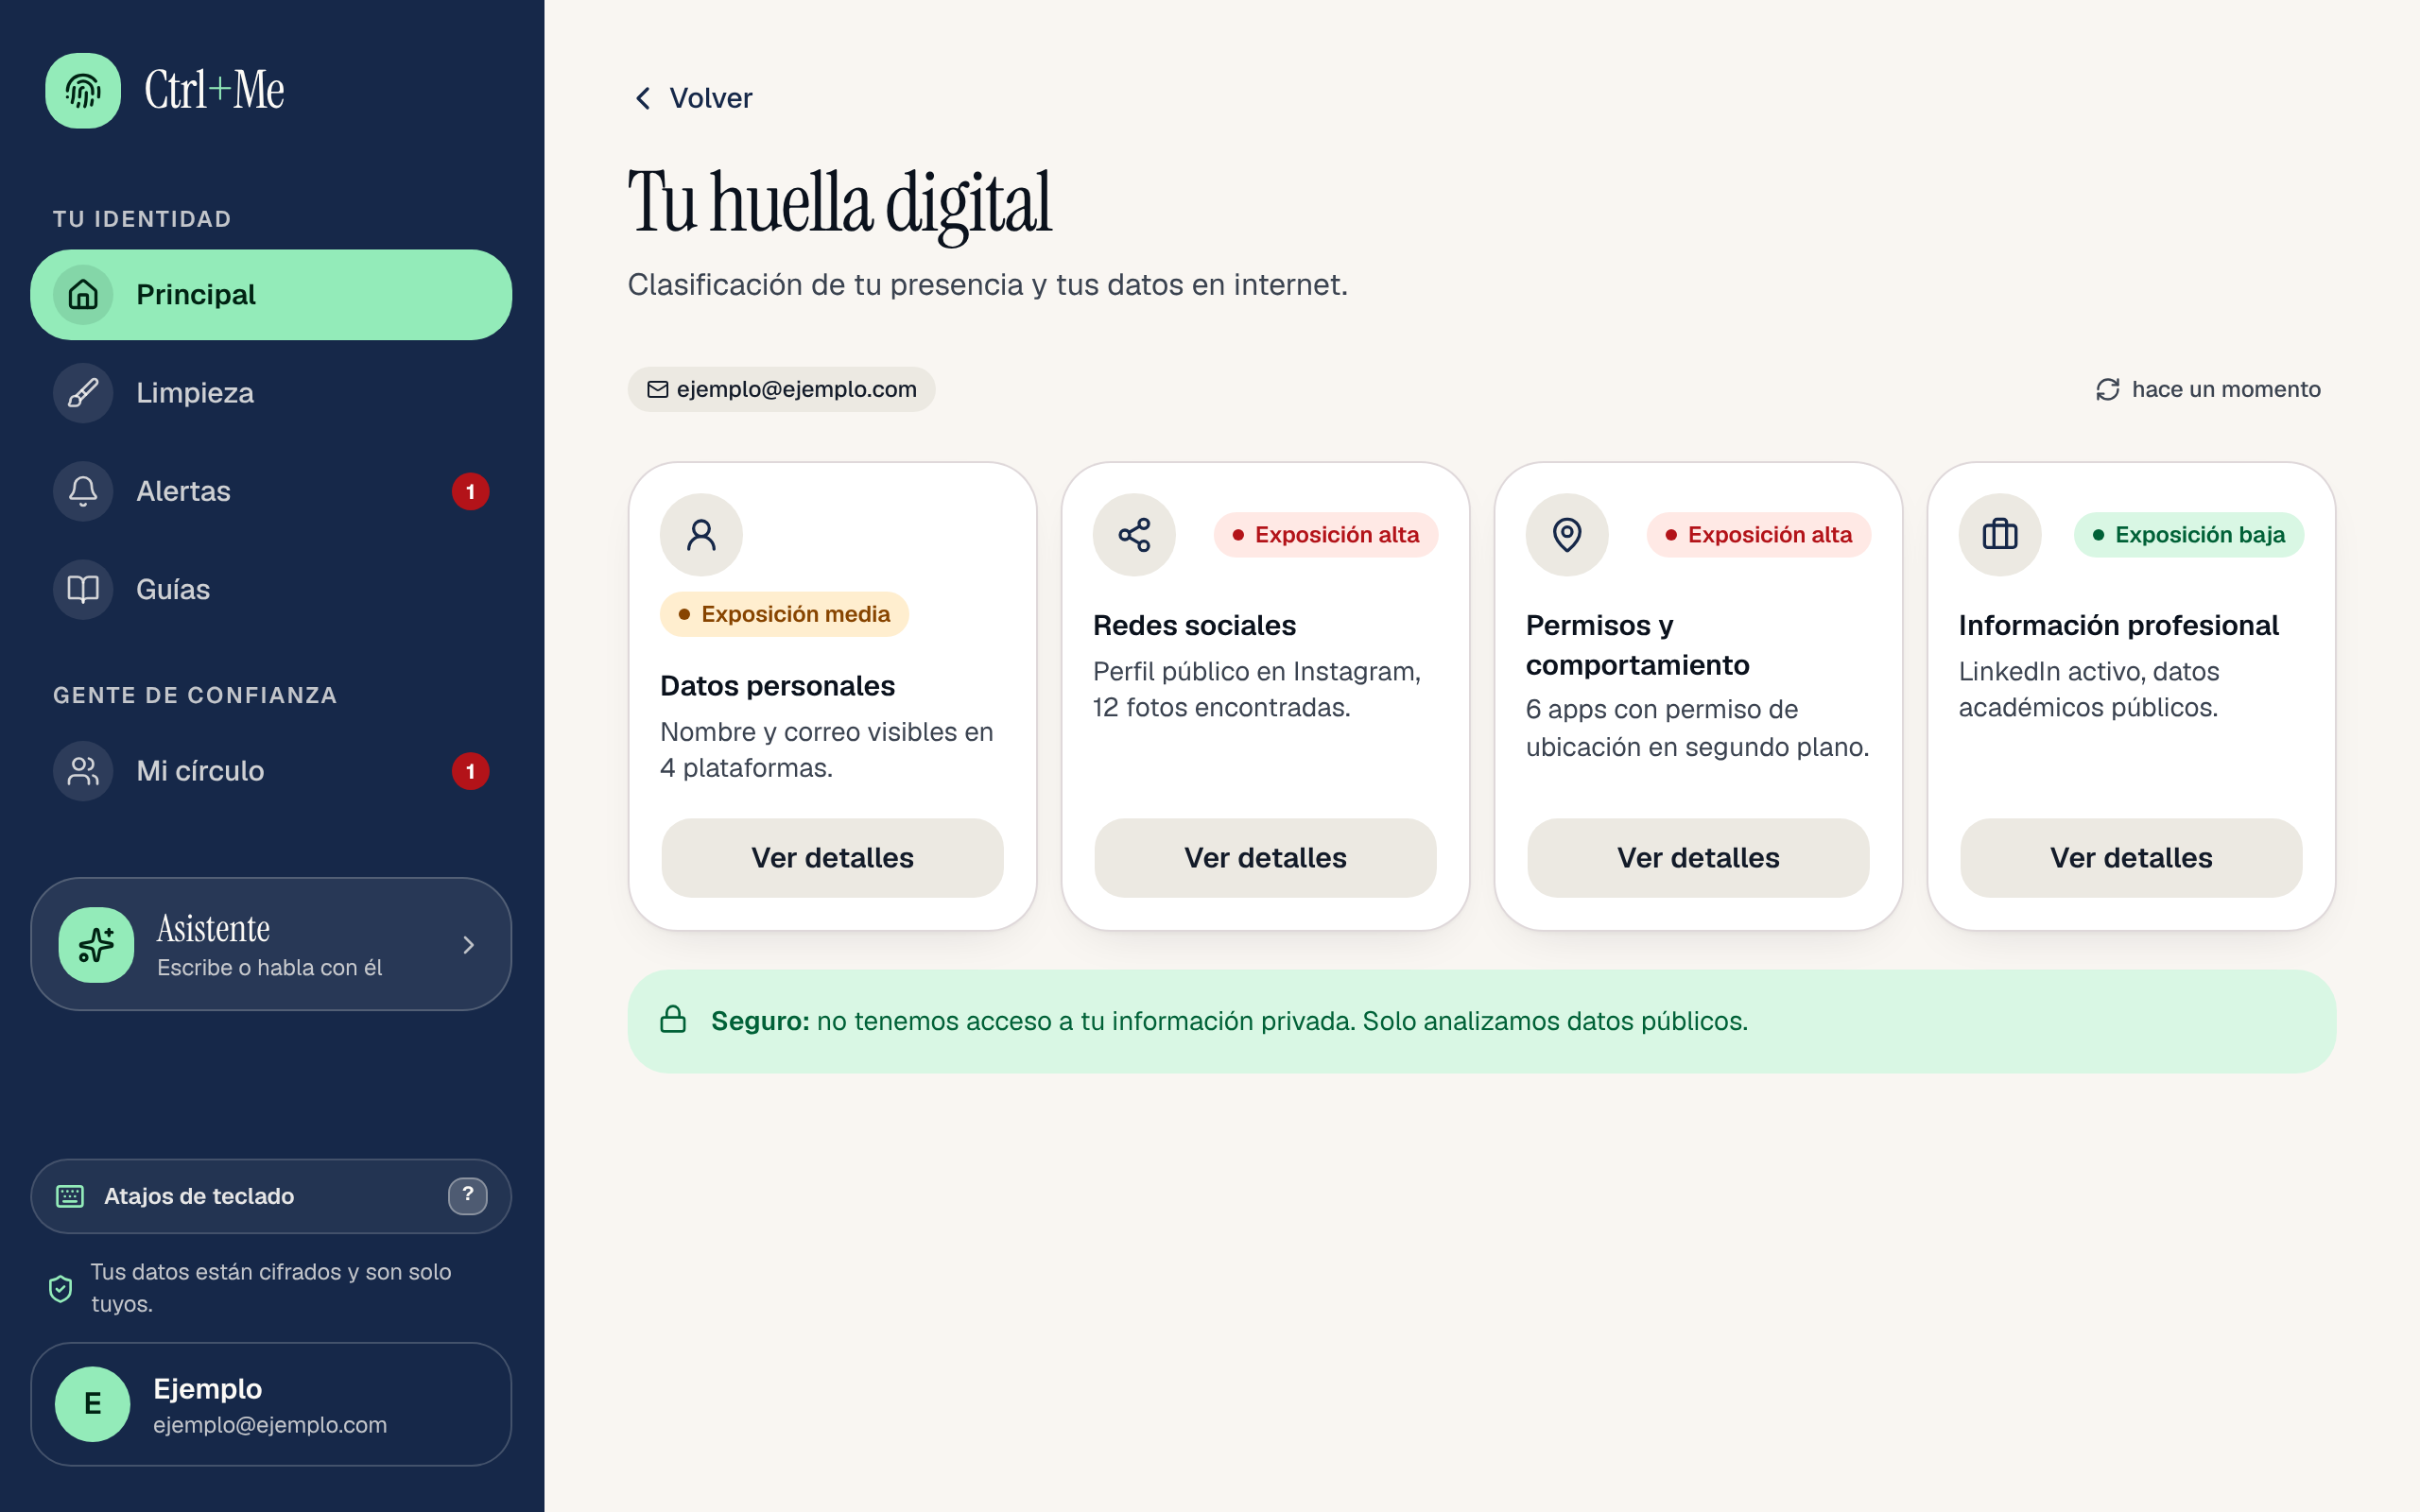
\includegraphics[width=\textwidth]{figuras-v3/v3_huella_web.png}
    \caption{Categorías de Tu huella digital (web)}
  \end{subfigure}
  \hfill
  \begin{subfigure}[b]{0.48\textwidth}
    \centering
    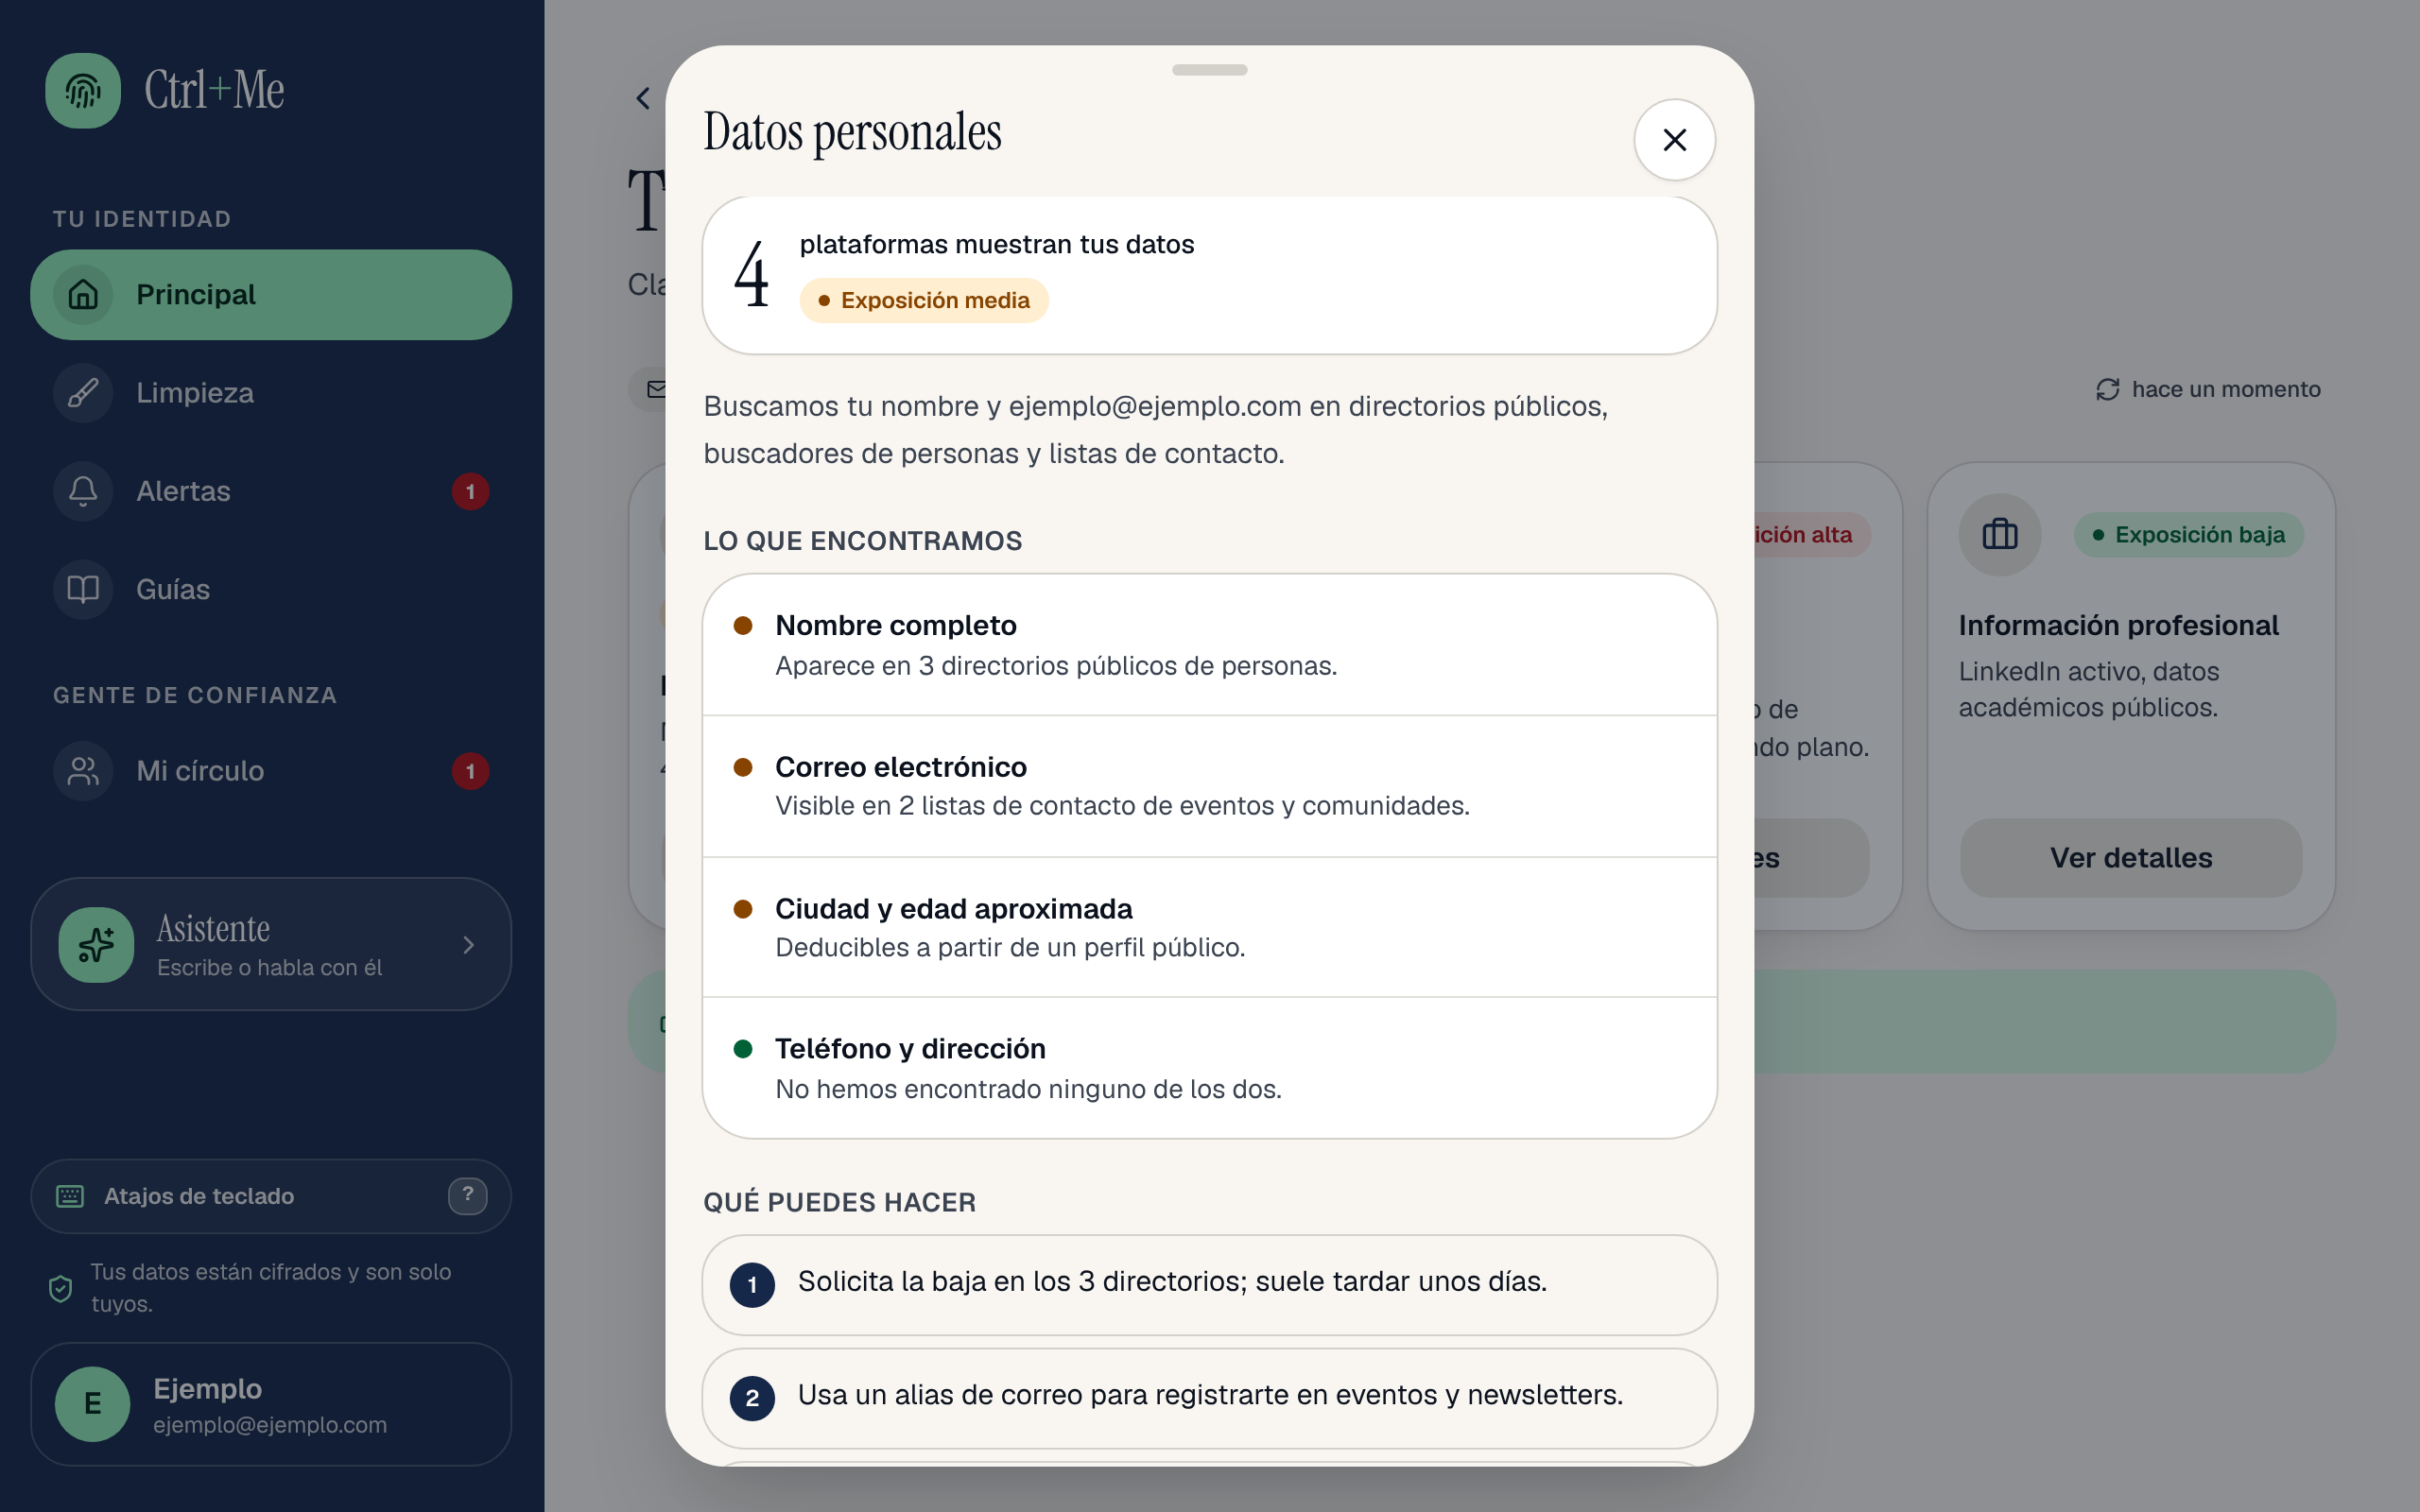
\includegraphics[width=\textwidth]{figuras-v3/v3_huella_modal_web.png}
    \caption{Detalle de categoría con botón \texttt{X} contrastado (web)}
  \end{subfigure}
  \\[0.75em]
  \begin{subfigure}[b]{0.30\textwidth}
    \centering
    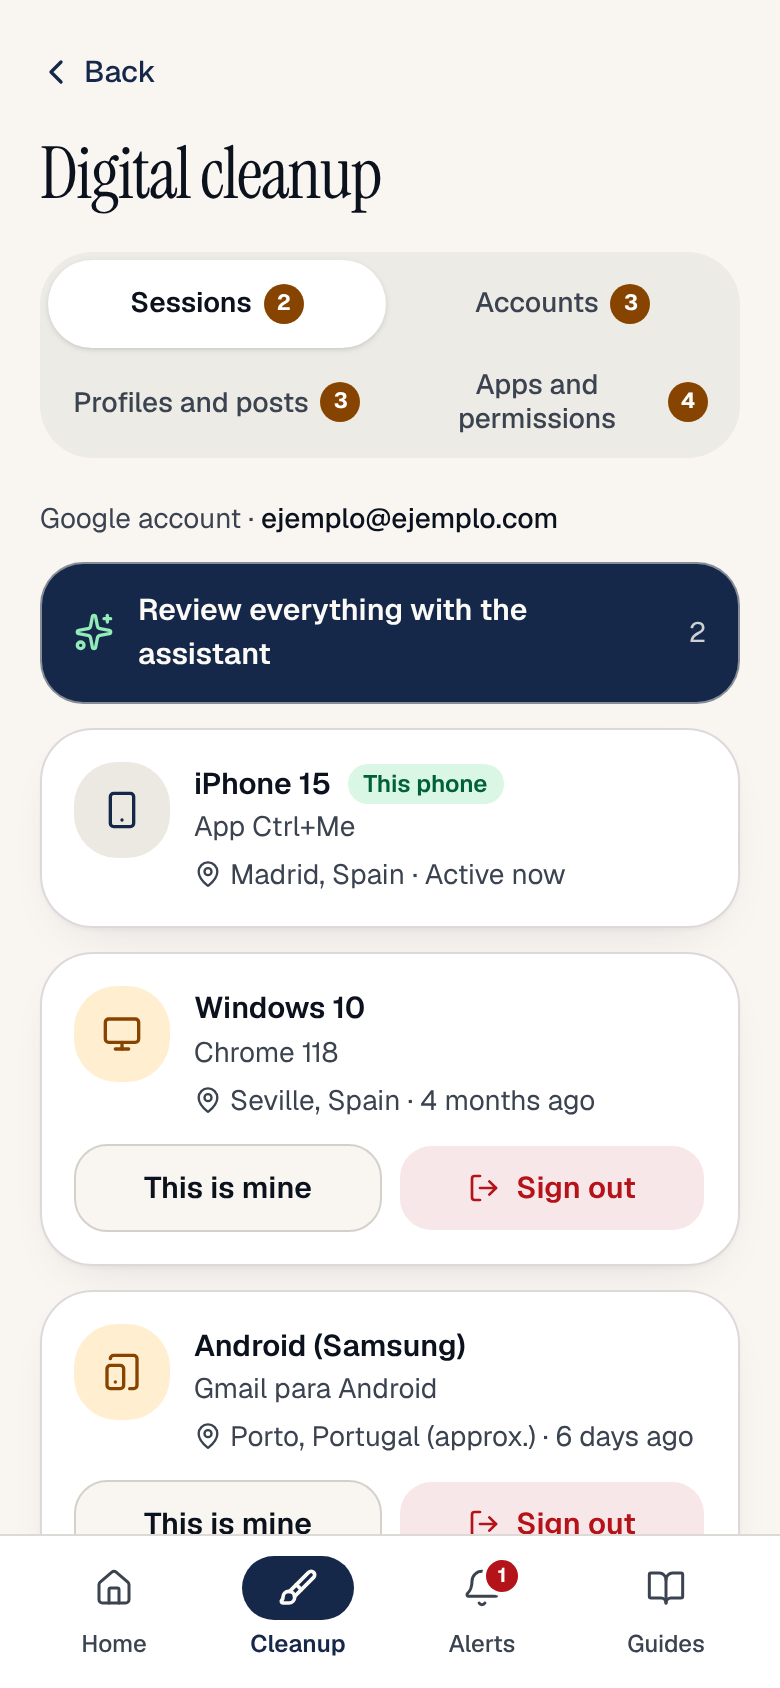
\includegraphics[width=\textwidth]{figuras-v3/v3_limpieza_en_movil.png}
    \caption{Limpieza digital en inglés (móvil)}
  \end{subfigure}
  \hfill
  \begin{subfigure}[b]{0.64\textwidth}
    \centering
    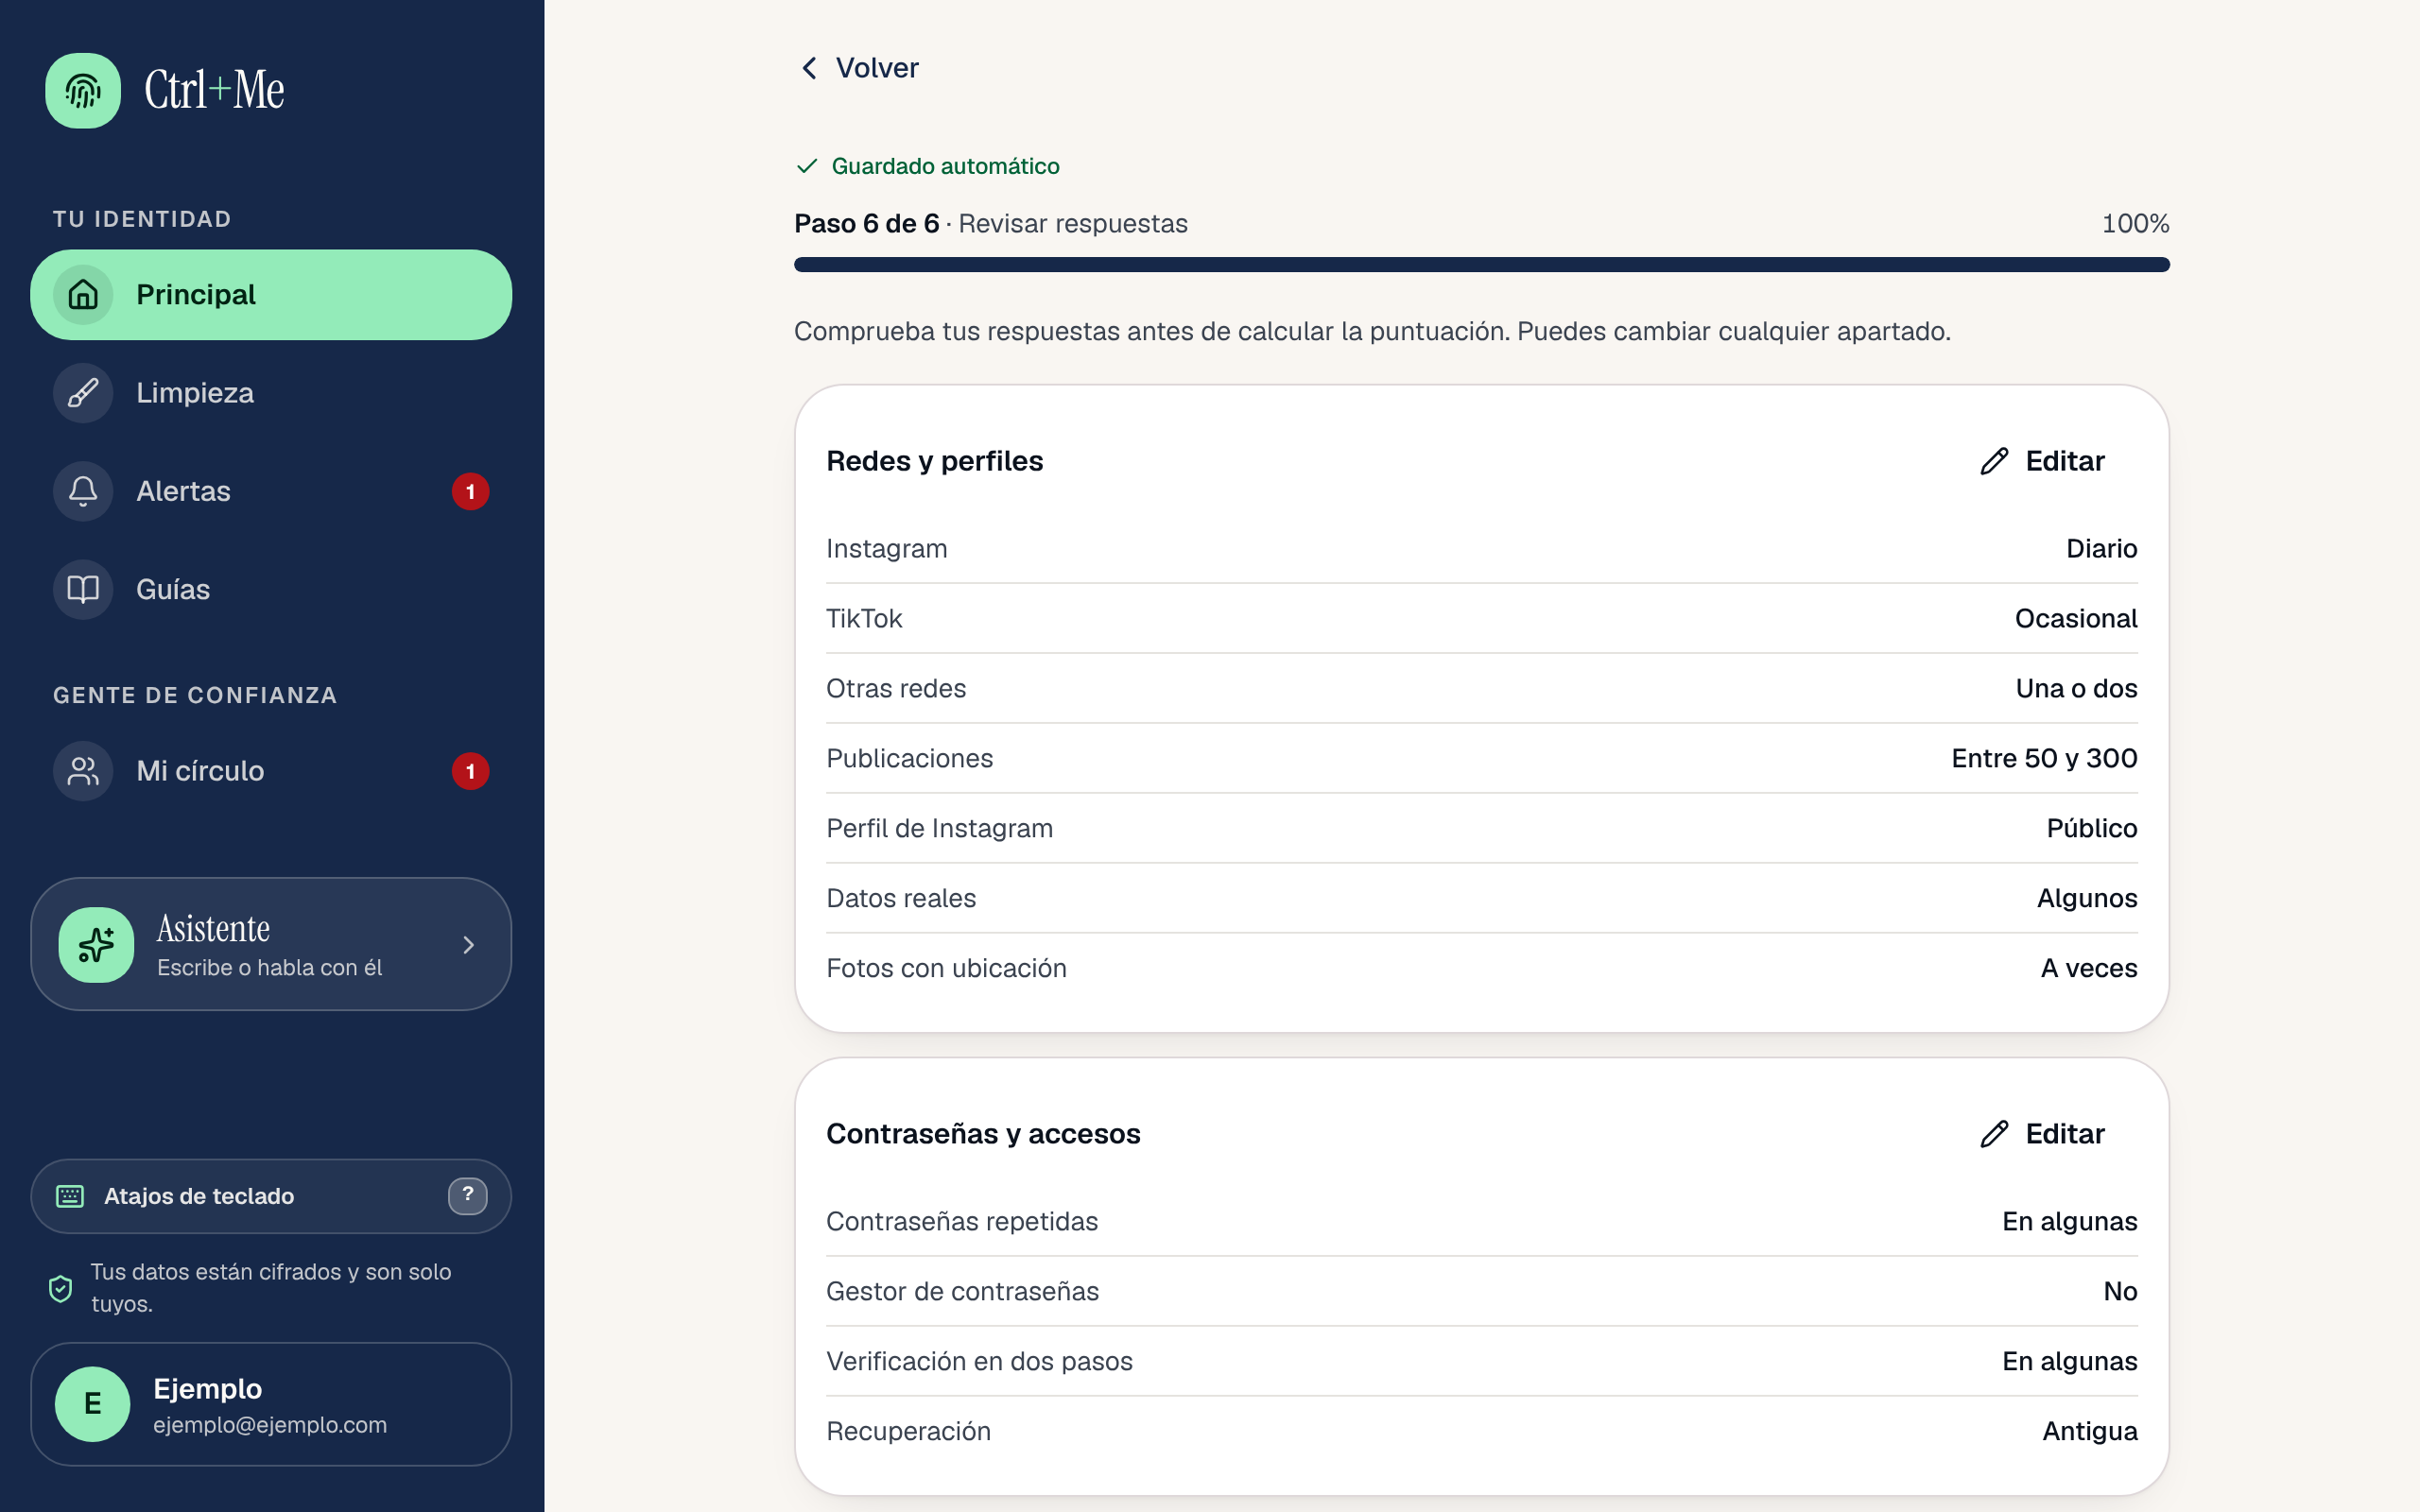
\includegraphics[width=\textwidth]{figuras-v3/v3_evaluacion_revision_web.png}
    \caption{Revisión de respuestas (Paso 6 de 6) con autoguardado (web)}
  \end{subfigure}
  \caption{Huella digital, limpieza móvil en inglés y revisión final de evaluación en v3.0.}
  \label{fig:v3-anexo-2}
\end{figure}

\begin{figure}[H]
  \centering
  \begin{subfigure}[b]{0.48\textwidth}
    \centering
    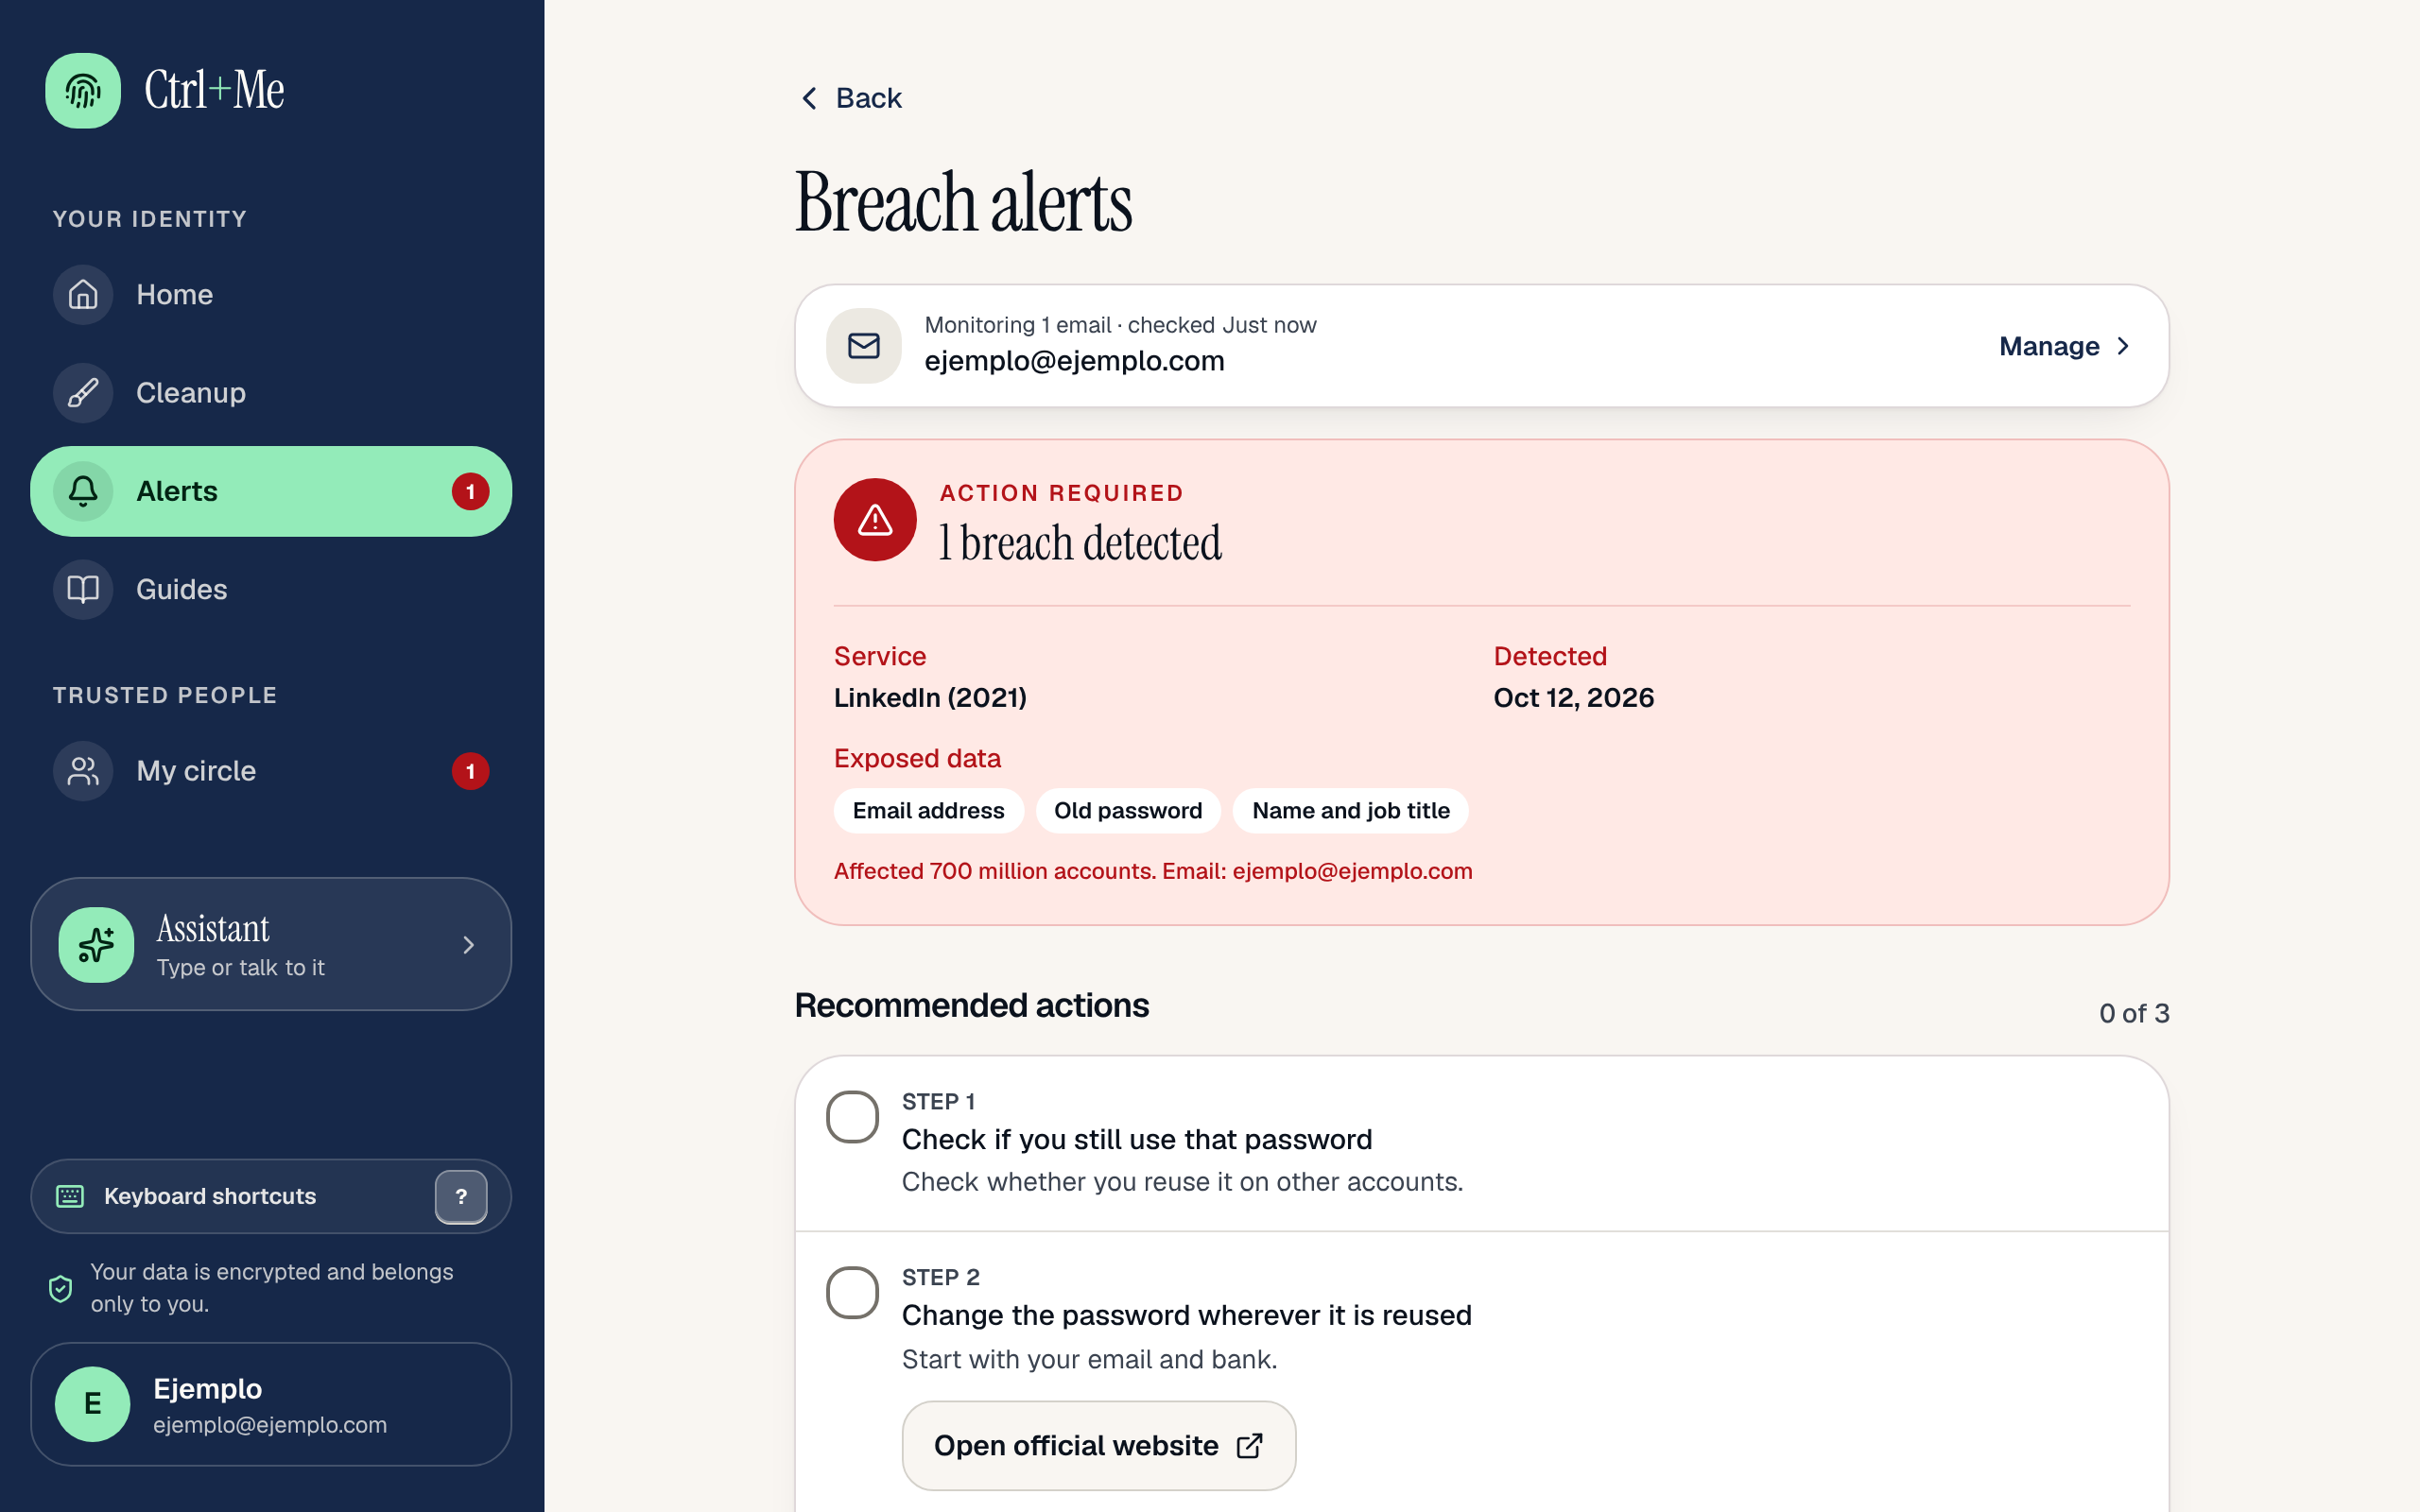
\includegraphics[width=\textwidth]{figuras-v3/v3_alertas_en_web.png}
    \caption{Alertas de filtraciones en inglés (web)}
  \end{subfigure}
  \hfill
  \begin{subfigure}[b]{0.27\textwidth}
    \centering
    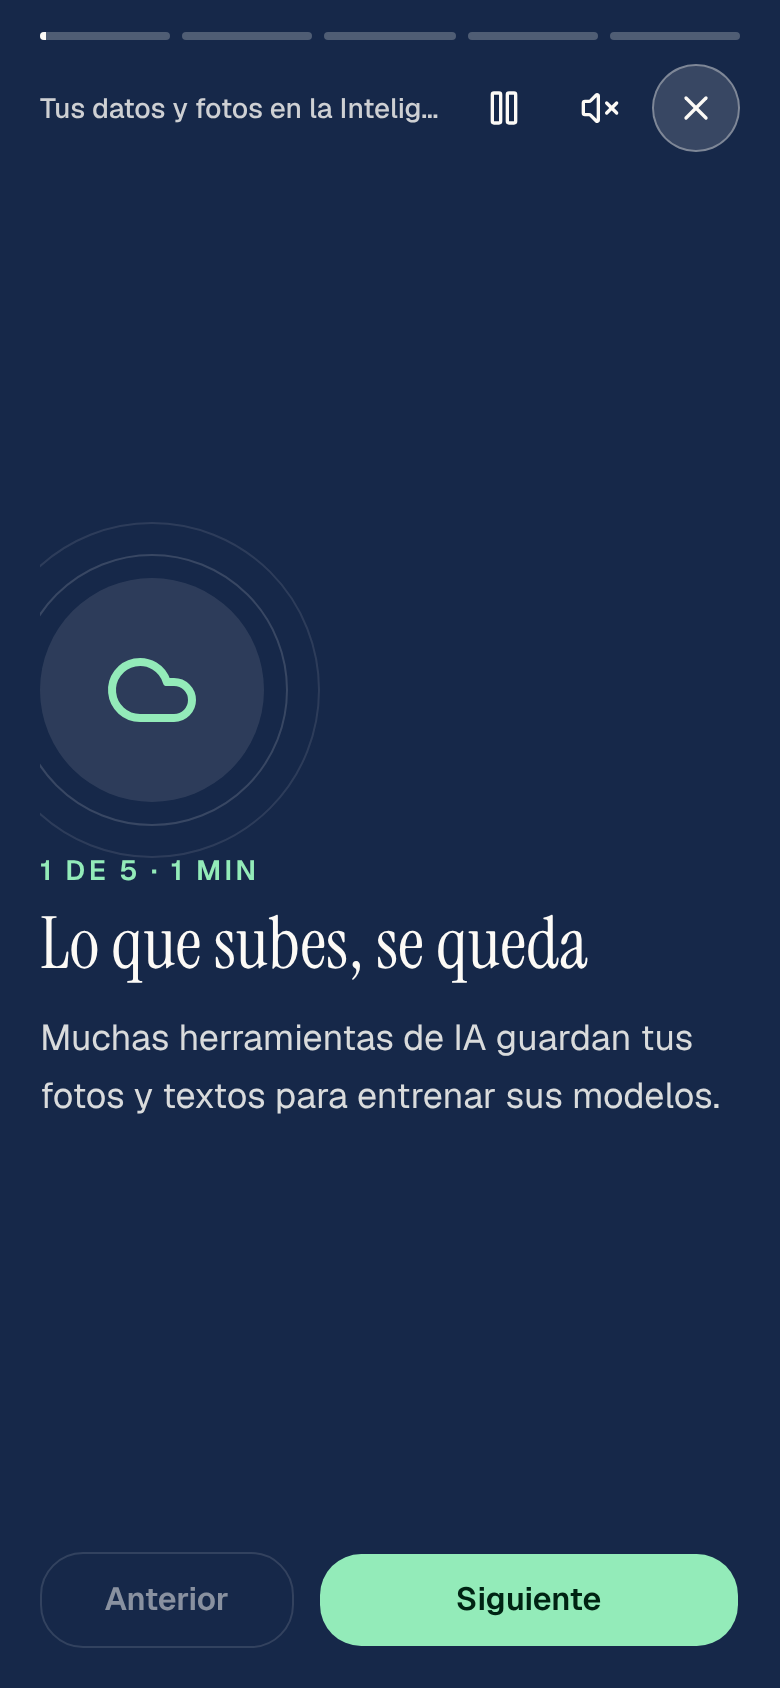
\includegraphics[width=\textwidth]{figuras-v3/v3_historia_movil.png}
    \caption{Historia visual multimodal (móvil)}
  \end{subfigure}
  \\[0.75em]
  \begin{subfigure}[b]{0.48\textwidth}
    \centering
    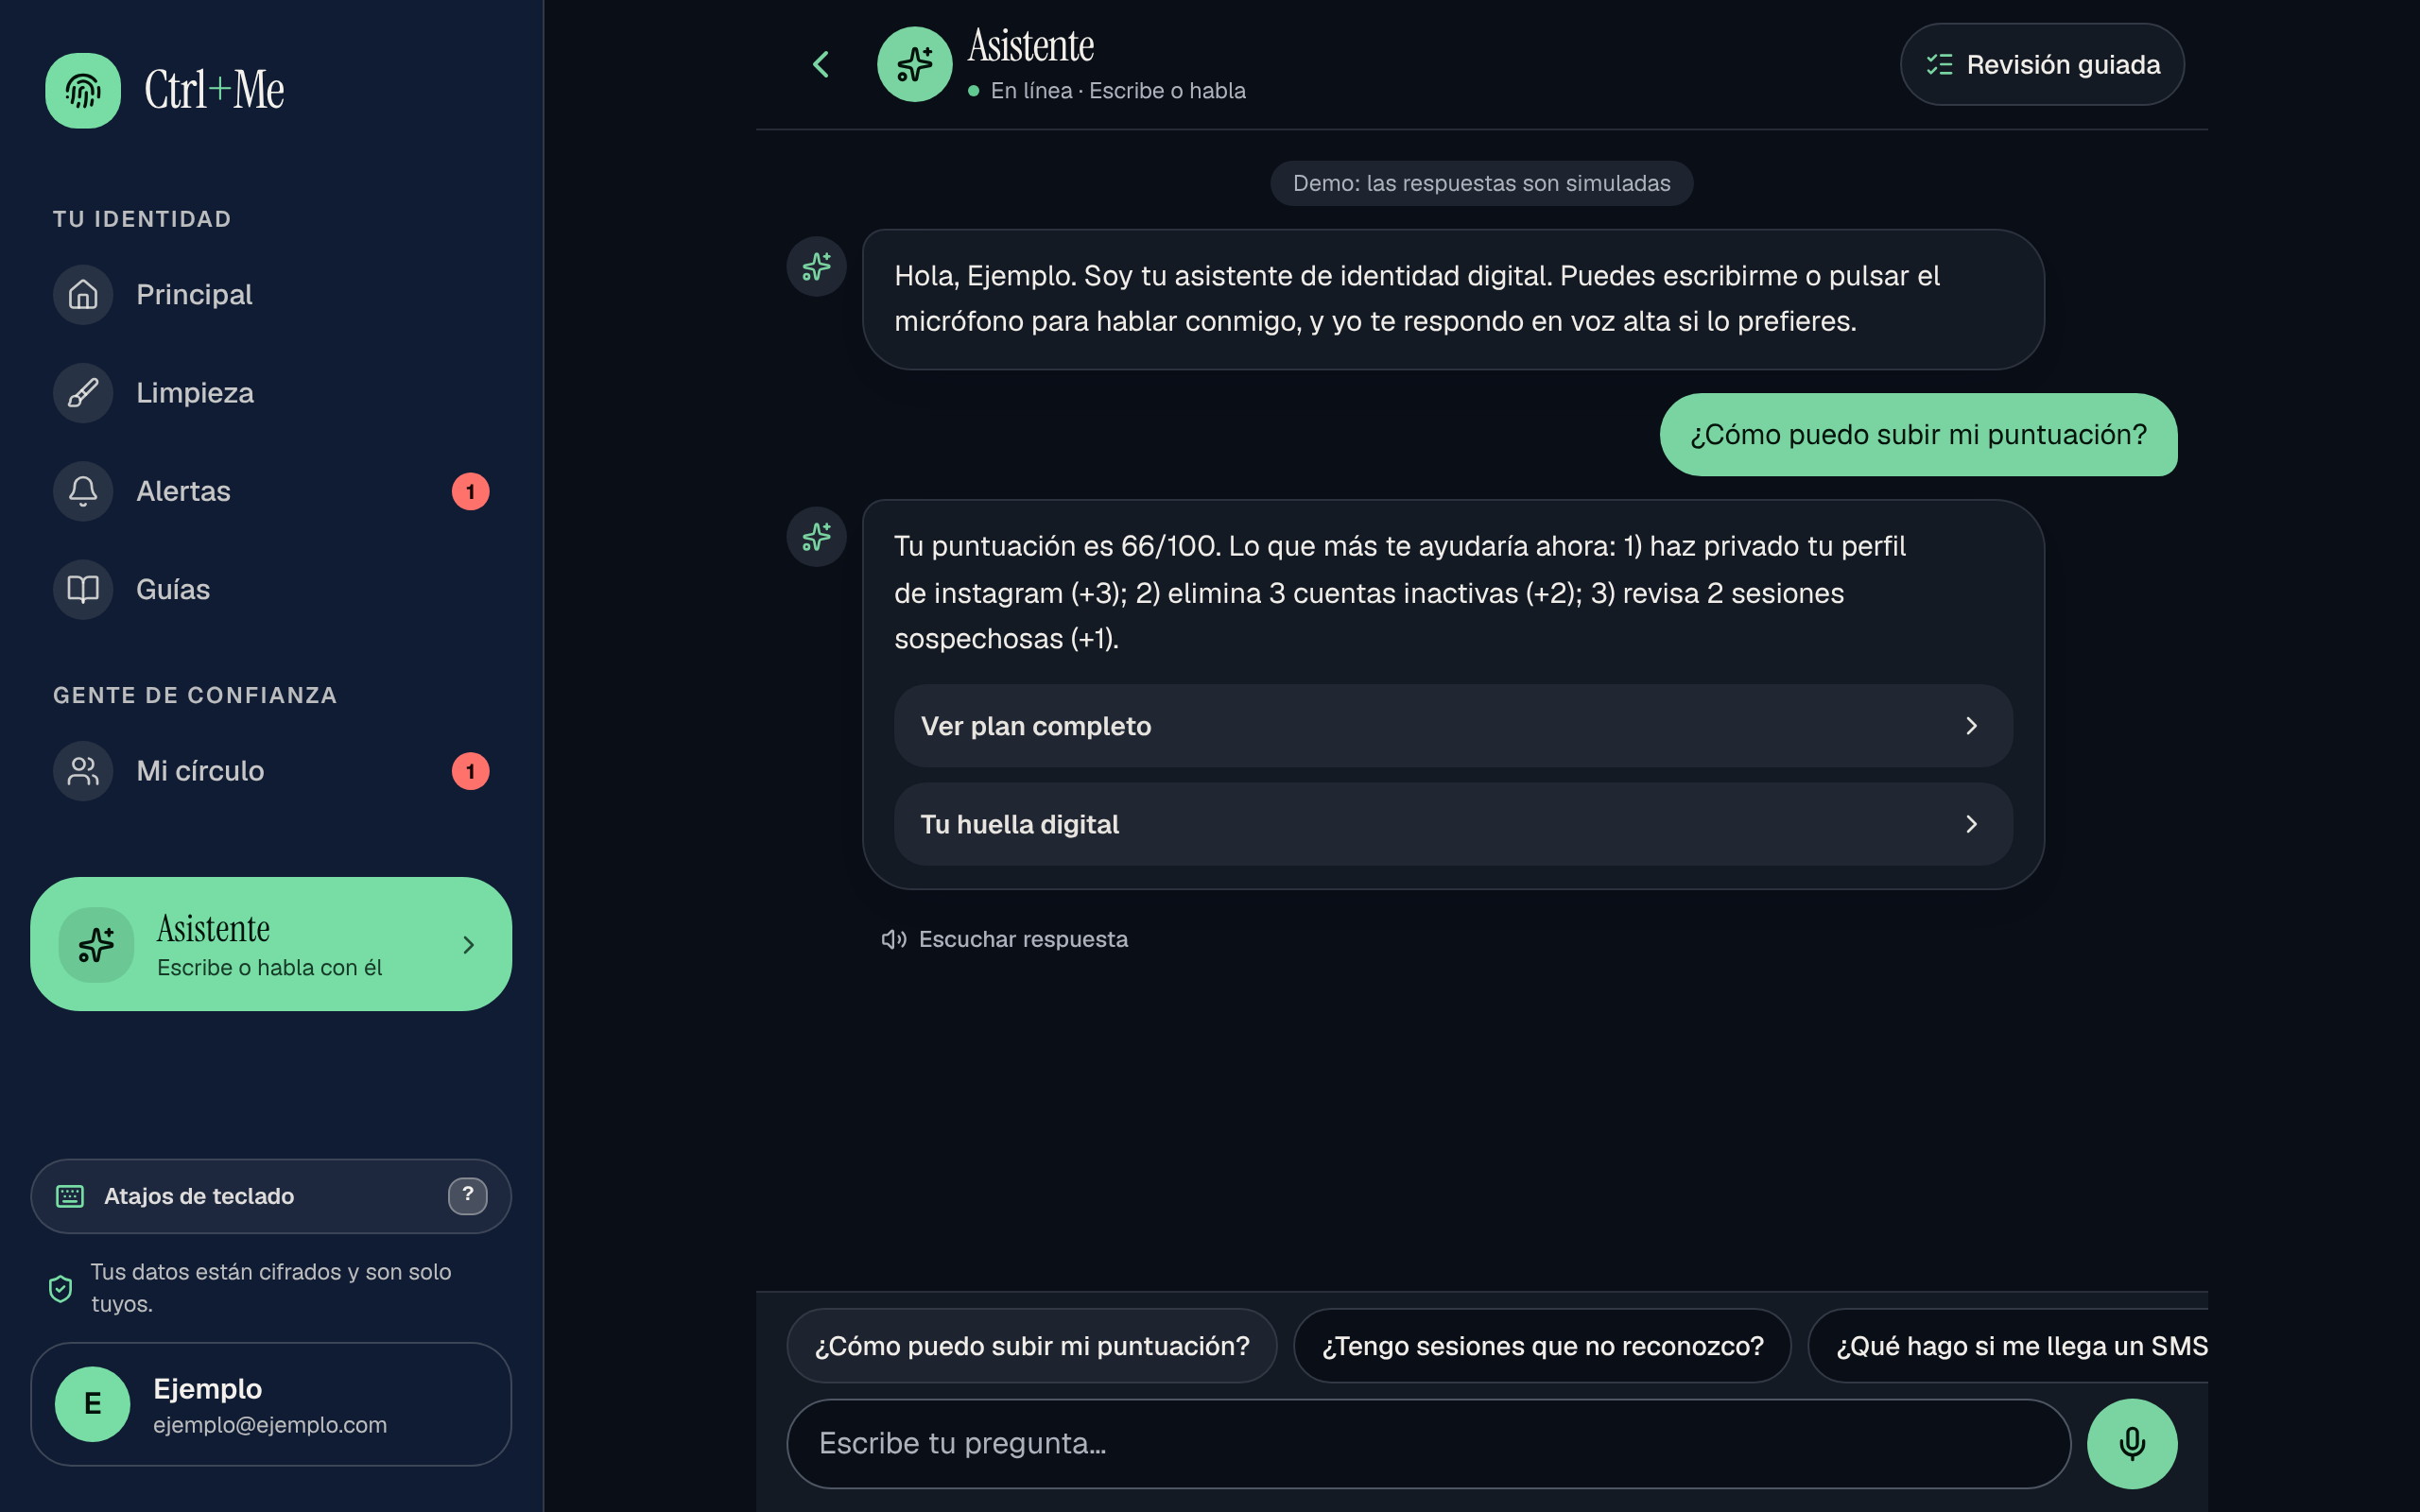
\includegraphics[width=\textwidth]{figuras-v3/v3_asistente_oscuro_web.png}
    \caption{Asistente conversacional en modo oscuro (web)}
  \end{subfigure}
  \hfill
  \begin{subfigure}[b]{0.48\textwidth}
    \centering
    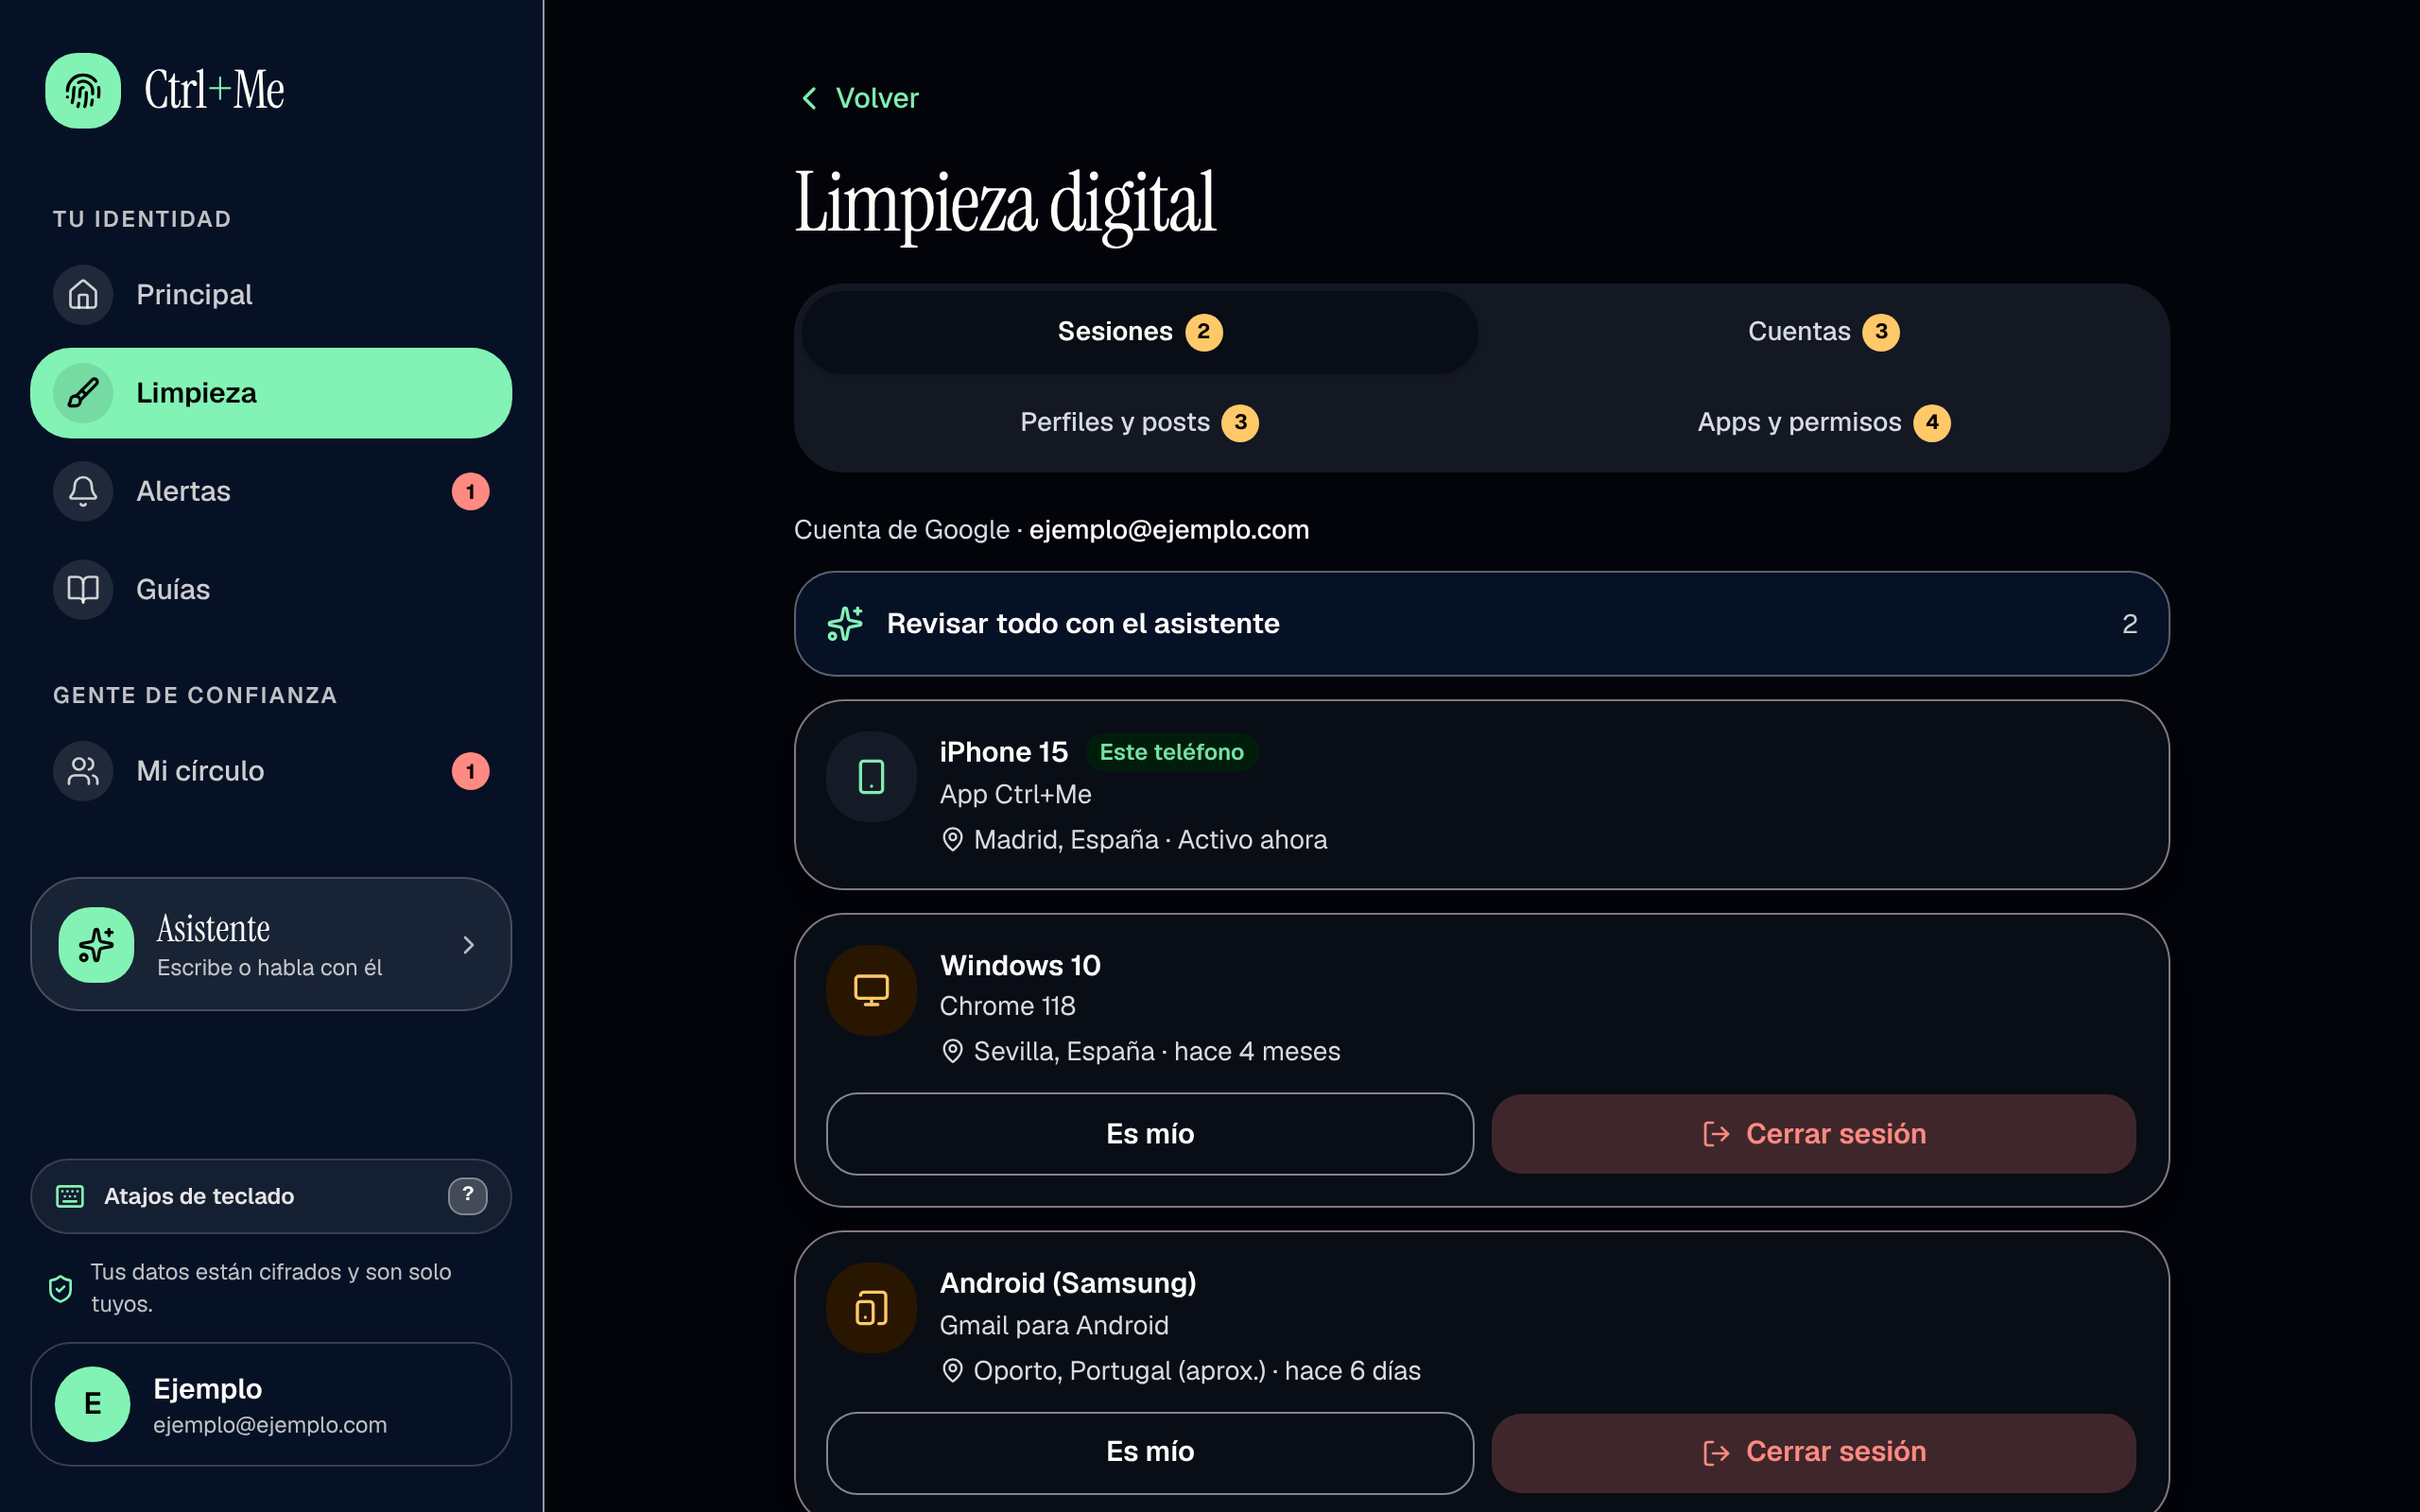
\includegraphics[width=\textwidth]{figuras-v3/v3_limpieza_oscuro_alto_contraste_web.png}
    \caption{Limpieza en oscuro y alto contraste (web)}
  \end{subfigure}
  \caption{Alertas en inglés, reproductor multimodal, asistente en modo oscuro y limpieza en oscuro con alto contraste.}
  \label{fig:v3-anexo-3}
\end{figure}

\begin{figure}[H]
  \centering
  \begin{subfigure}[b]{0.30\textwidth}
    \centering
    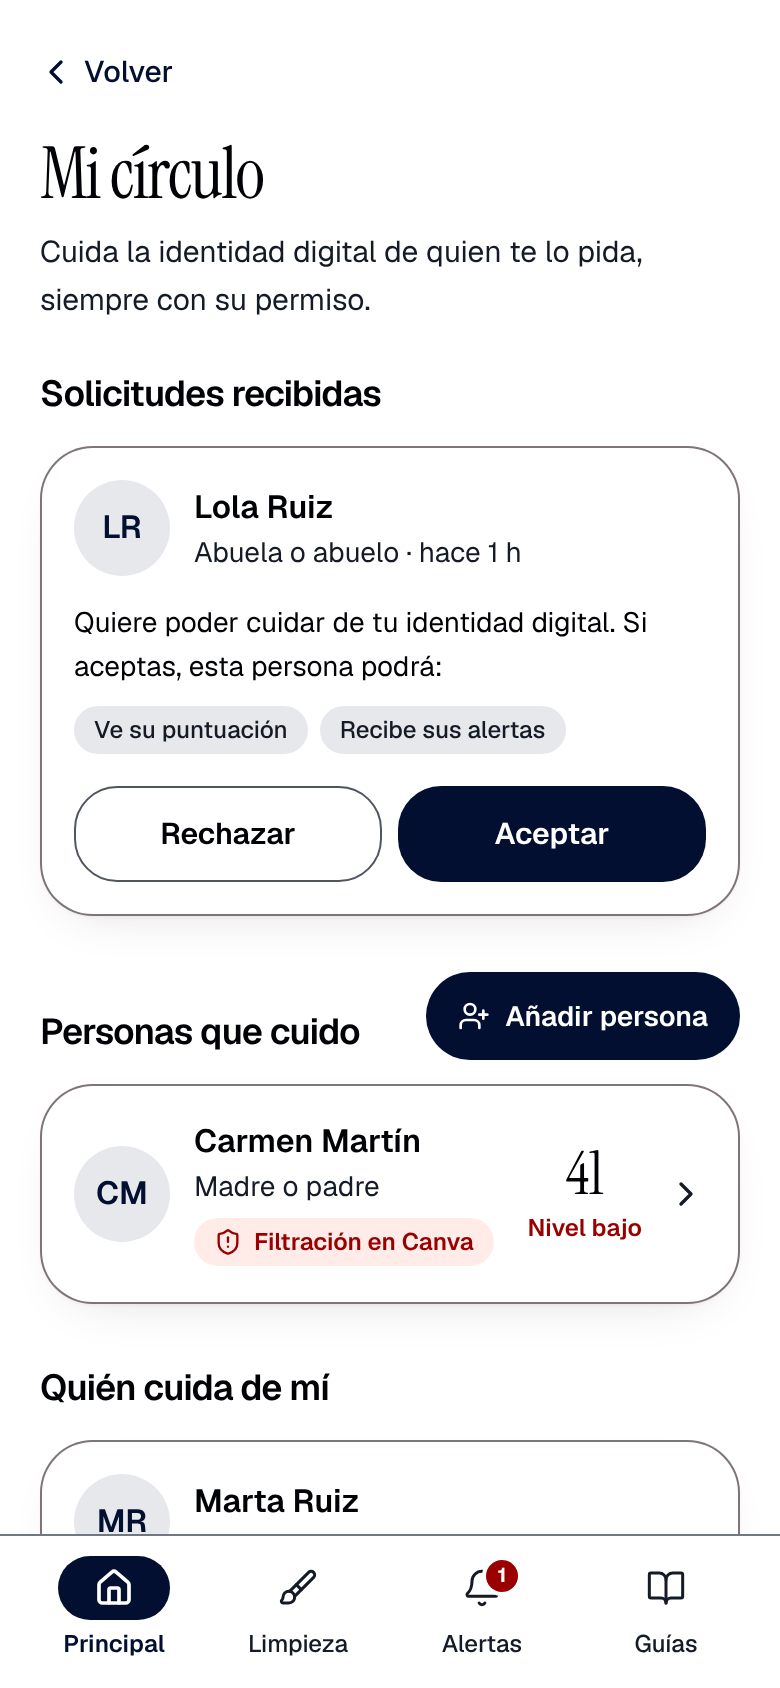
\includegraphics[width=\textwidth]{figuras-v3/v3_circulo_claro_alto_contraste_movil.png}
    \caption{Mi círculo en claro y alto contraste (móvil)}
  \end{subfigure}
  \hfill
  \begin{subfigure}[b]{0.64\textwidth}
    \centering
    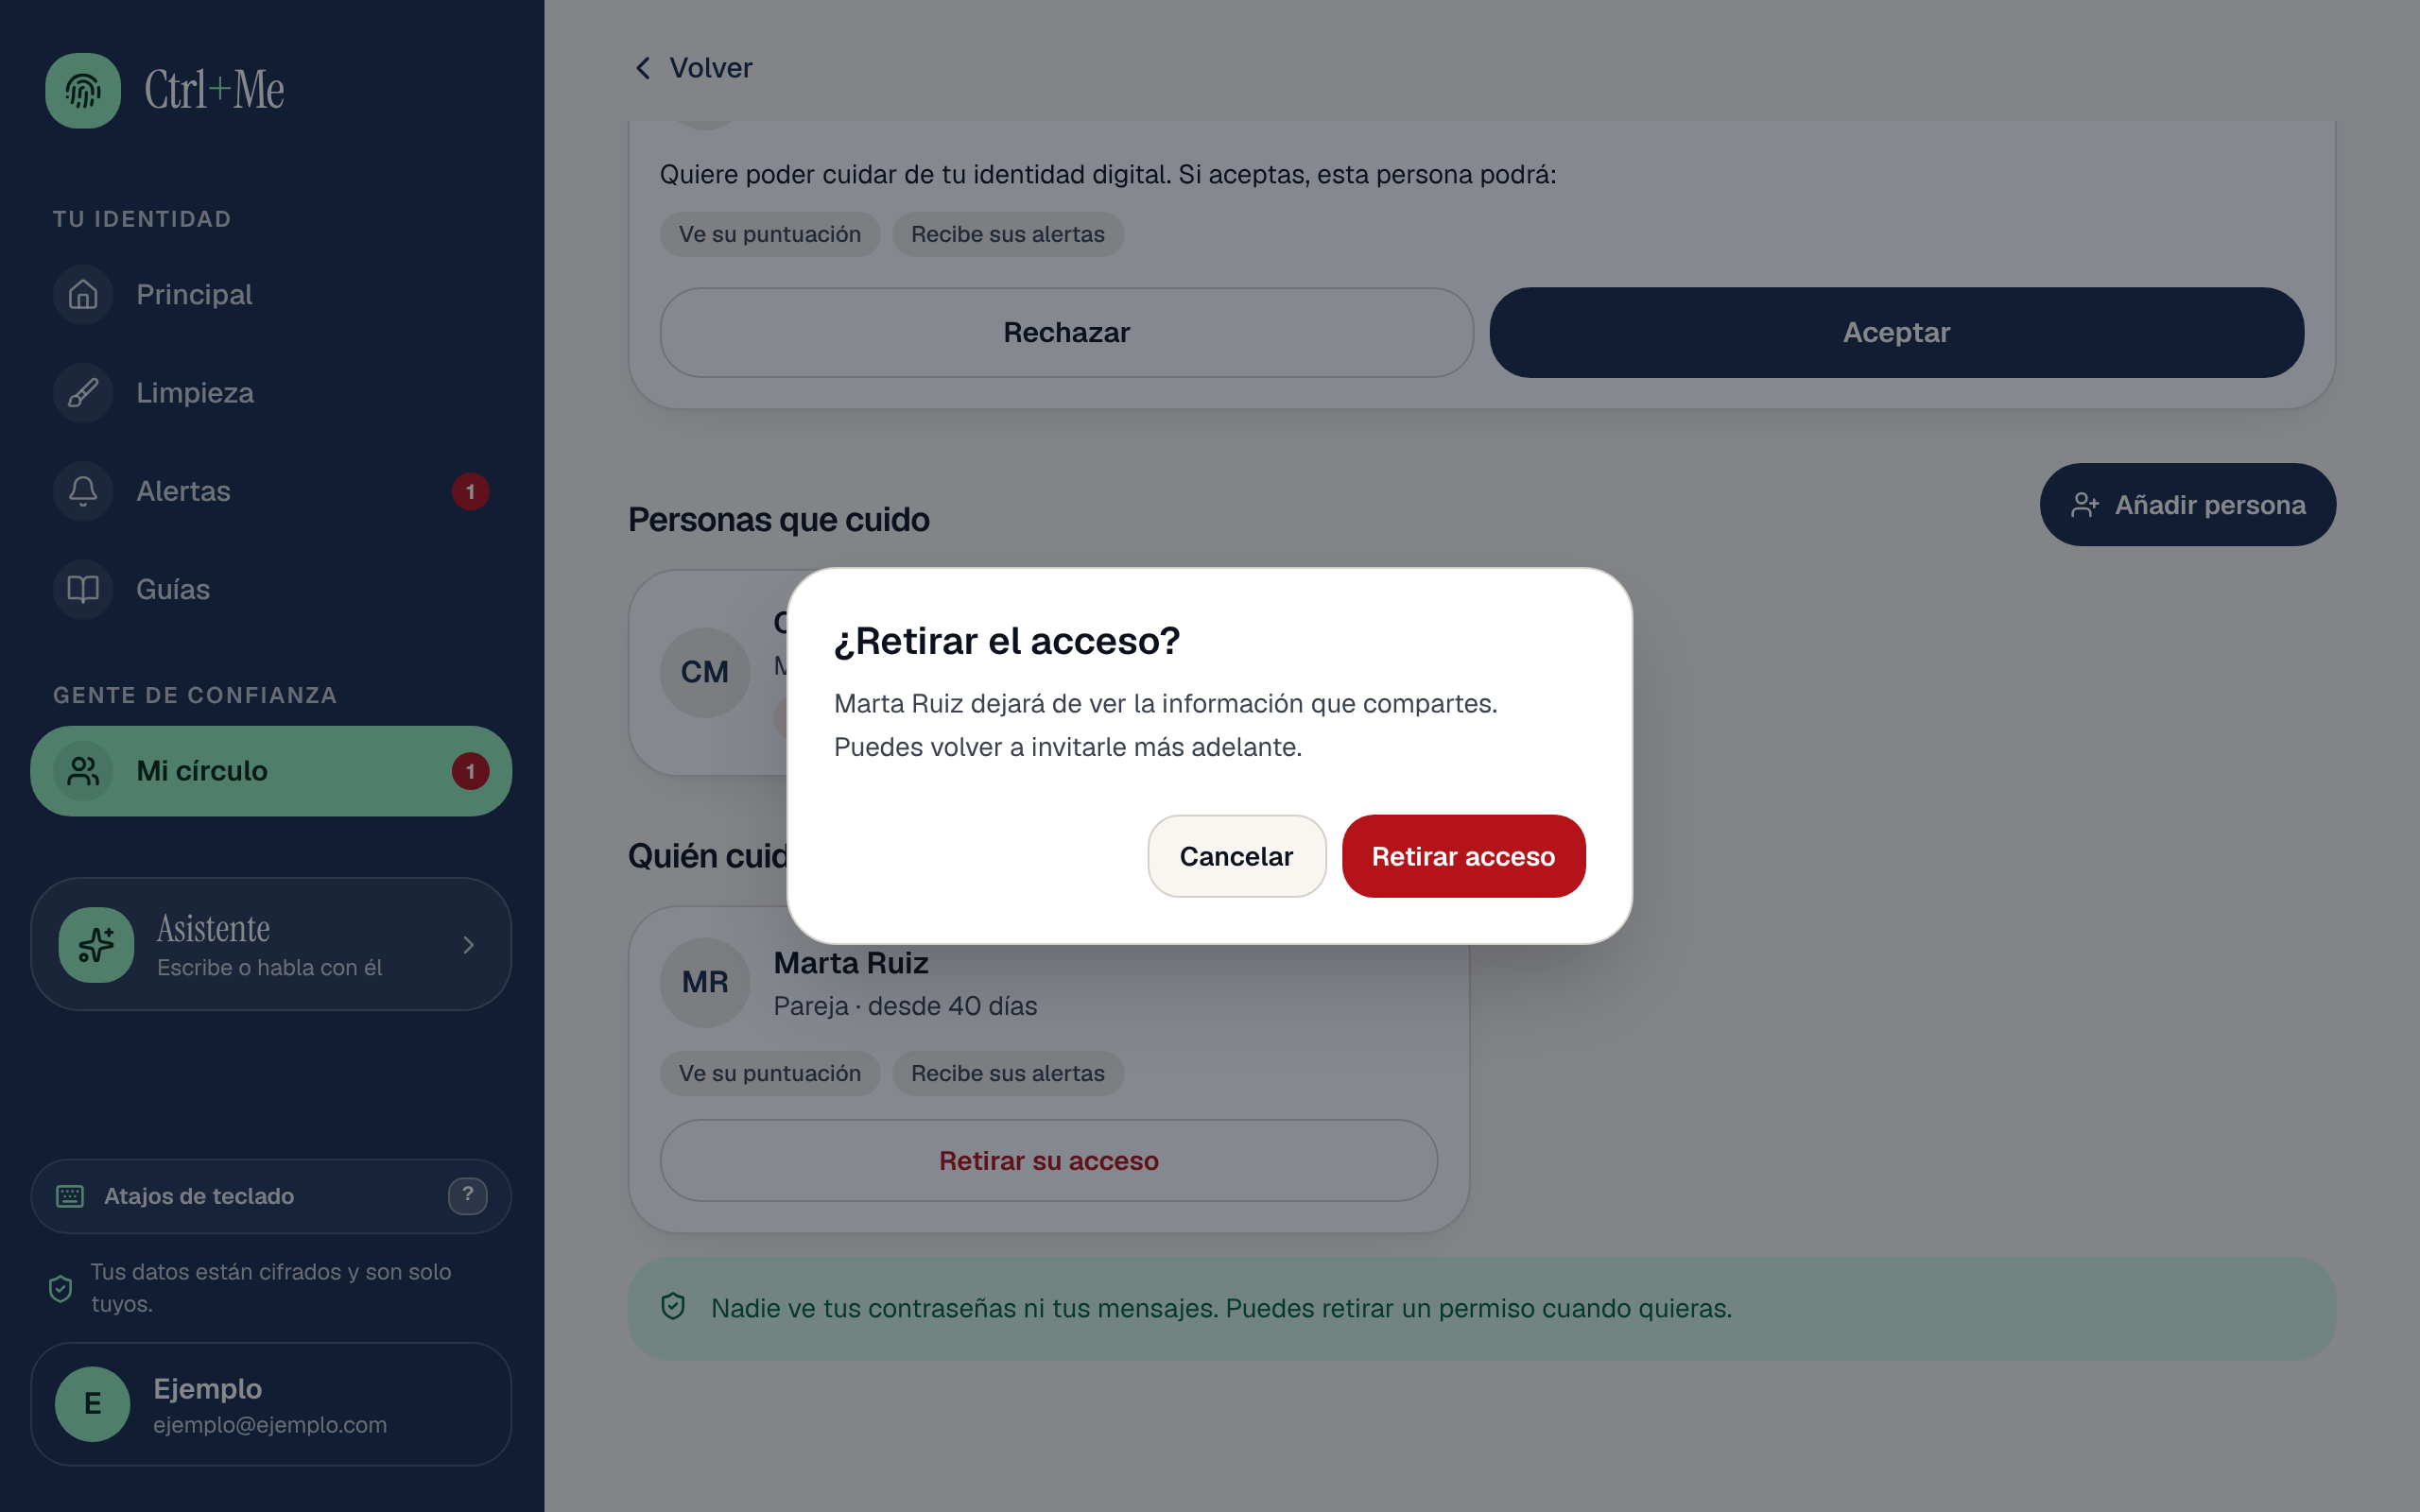
\includegraphics[width=\textwidth]{figuras-v3/v3_circulo_confirmar_web.png}
    \caption{Confirmación modal al retirar acceso en Mi círculo (web)}
  \end{subfigure}
  \\[0.75em]
  \begin{subfigure}[b]{0.48\textwidth}
    \centering
    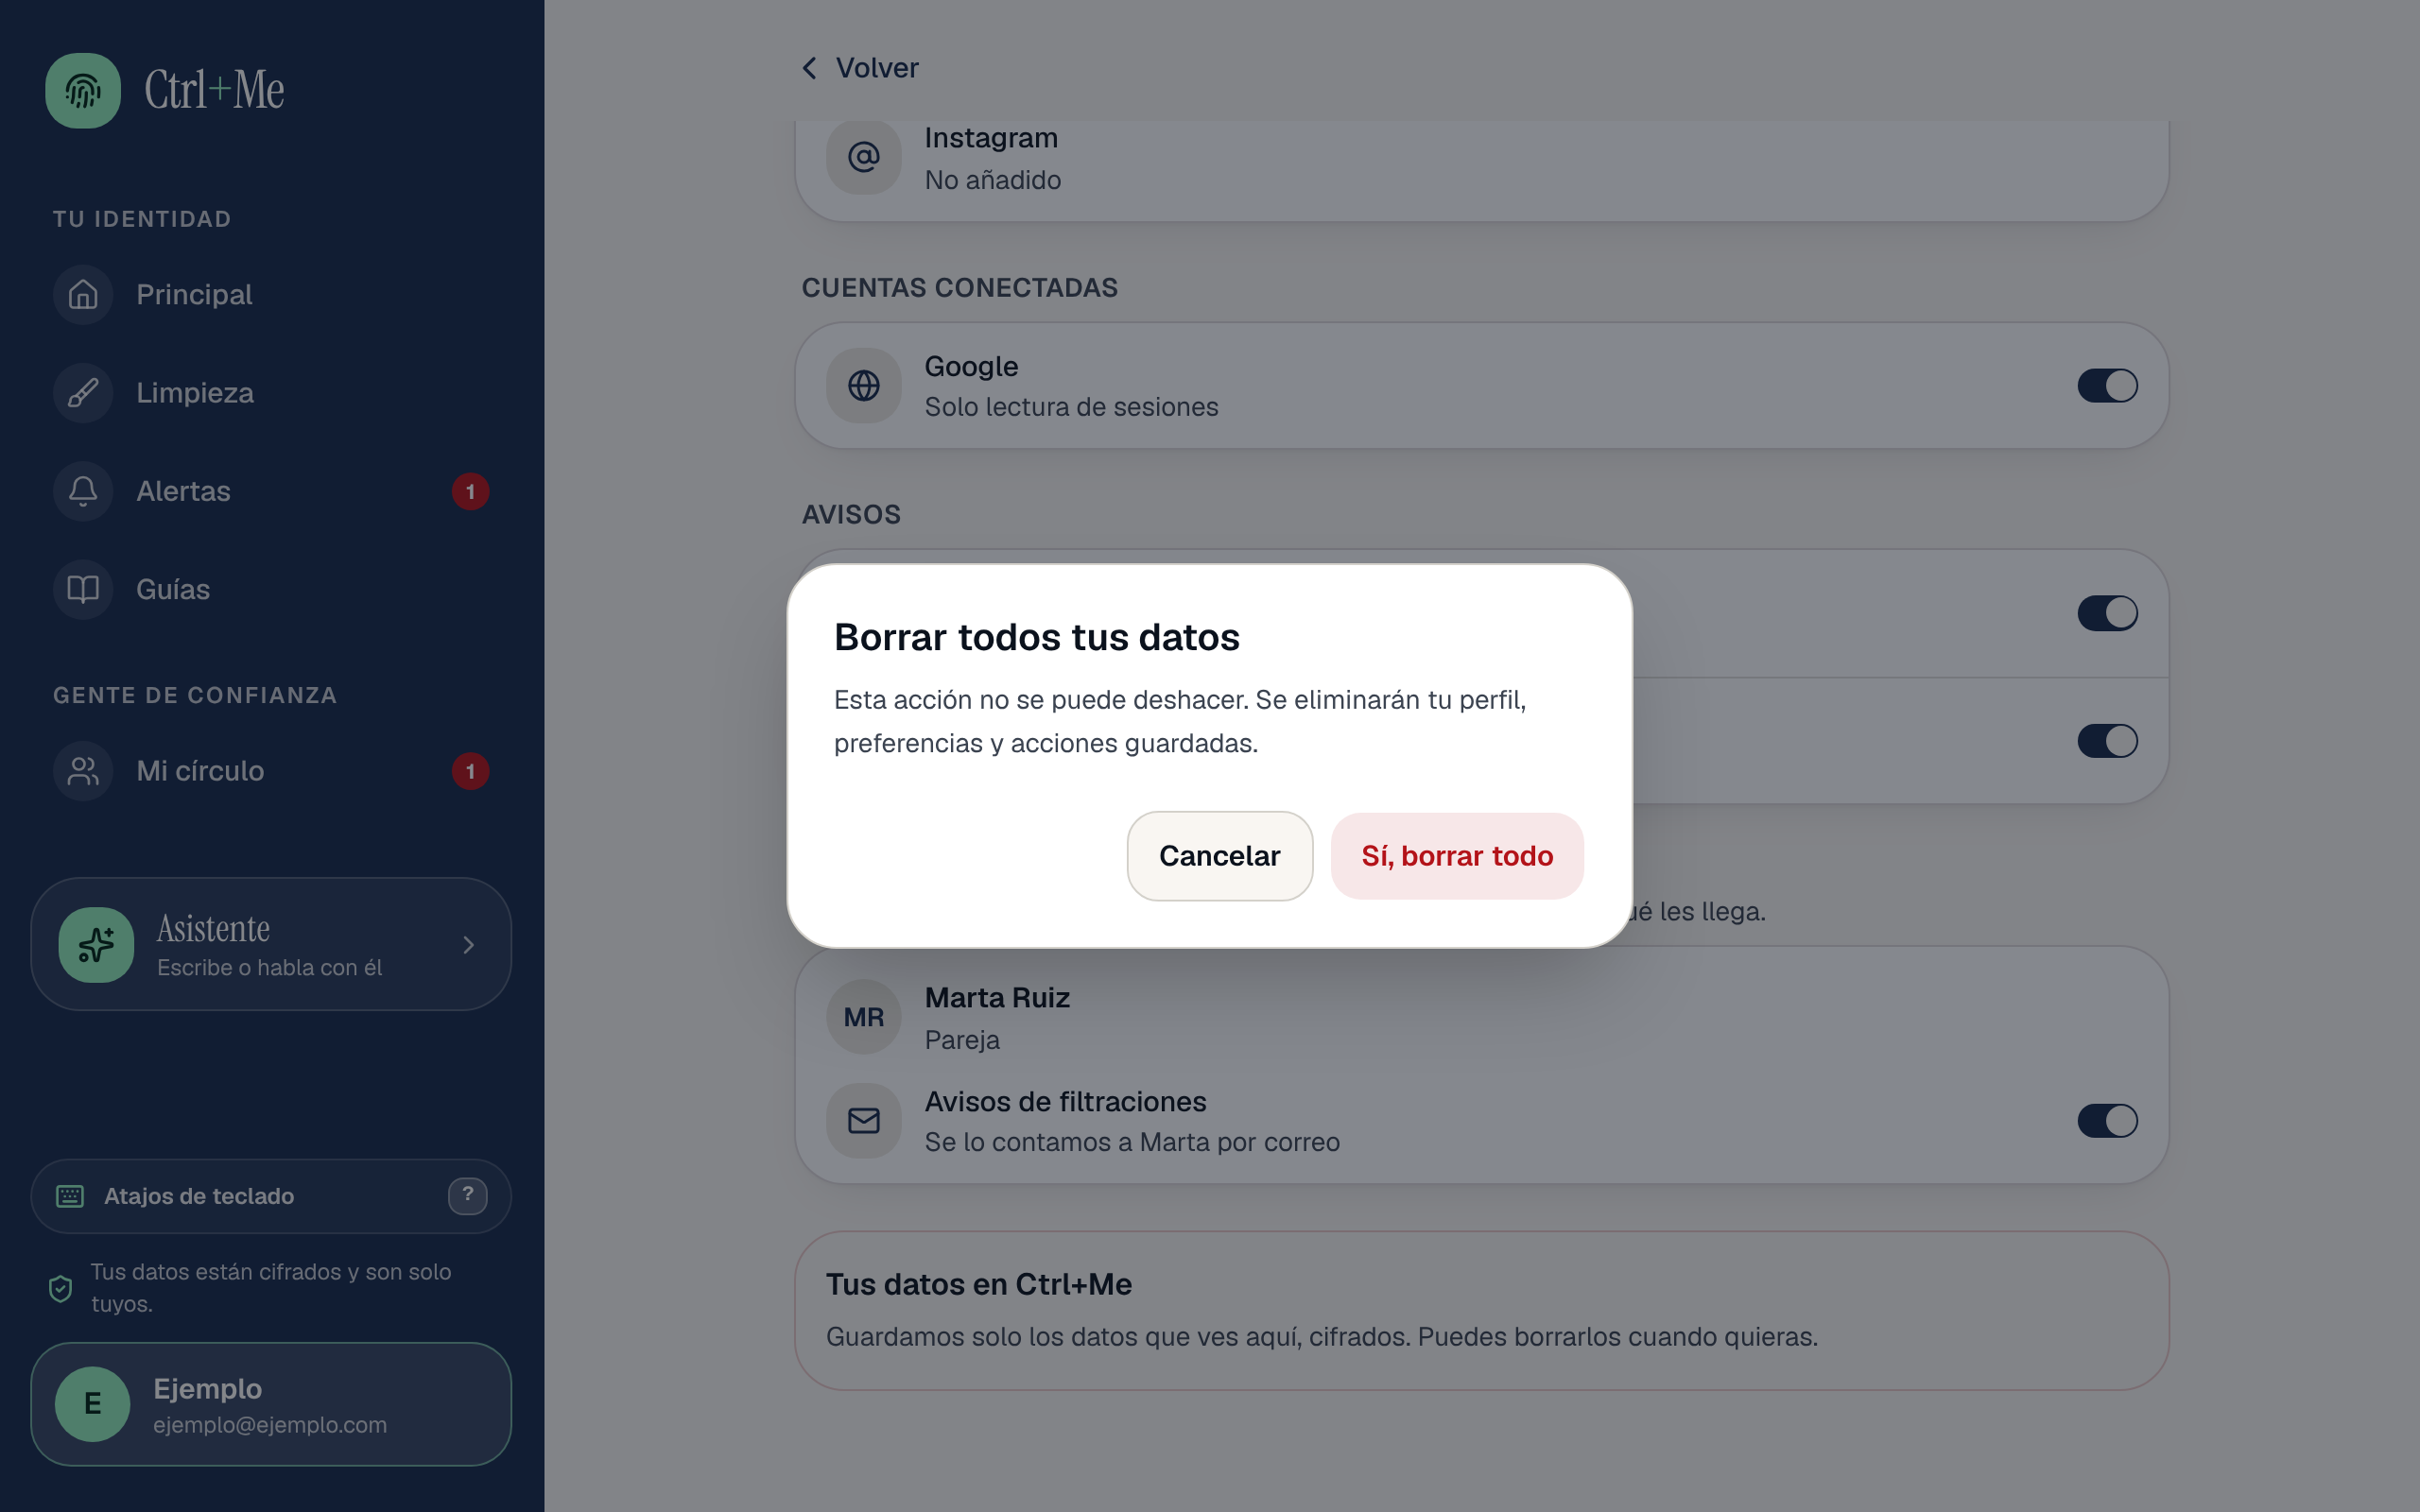
\includegraphics[width=\textwidth]{figuras-v3/v3_perfil_confirmar_borrar_web.png}
    \caption{Confirmación modal al borrar cuenta y datos (web)}
  \end{subfigure}
  \hfill
  \begin{subfigure}[b]{0.48\textwidth}
    \centering
    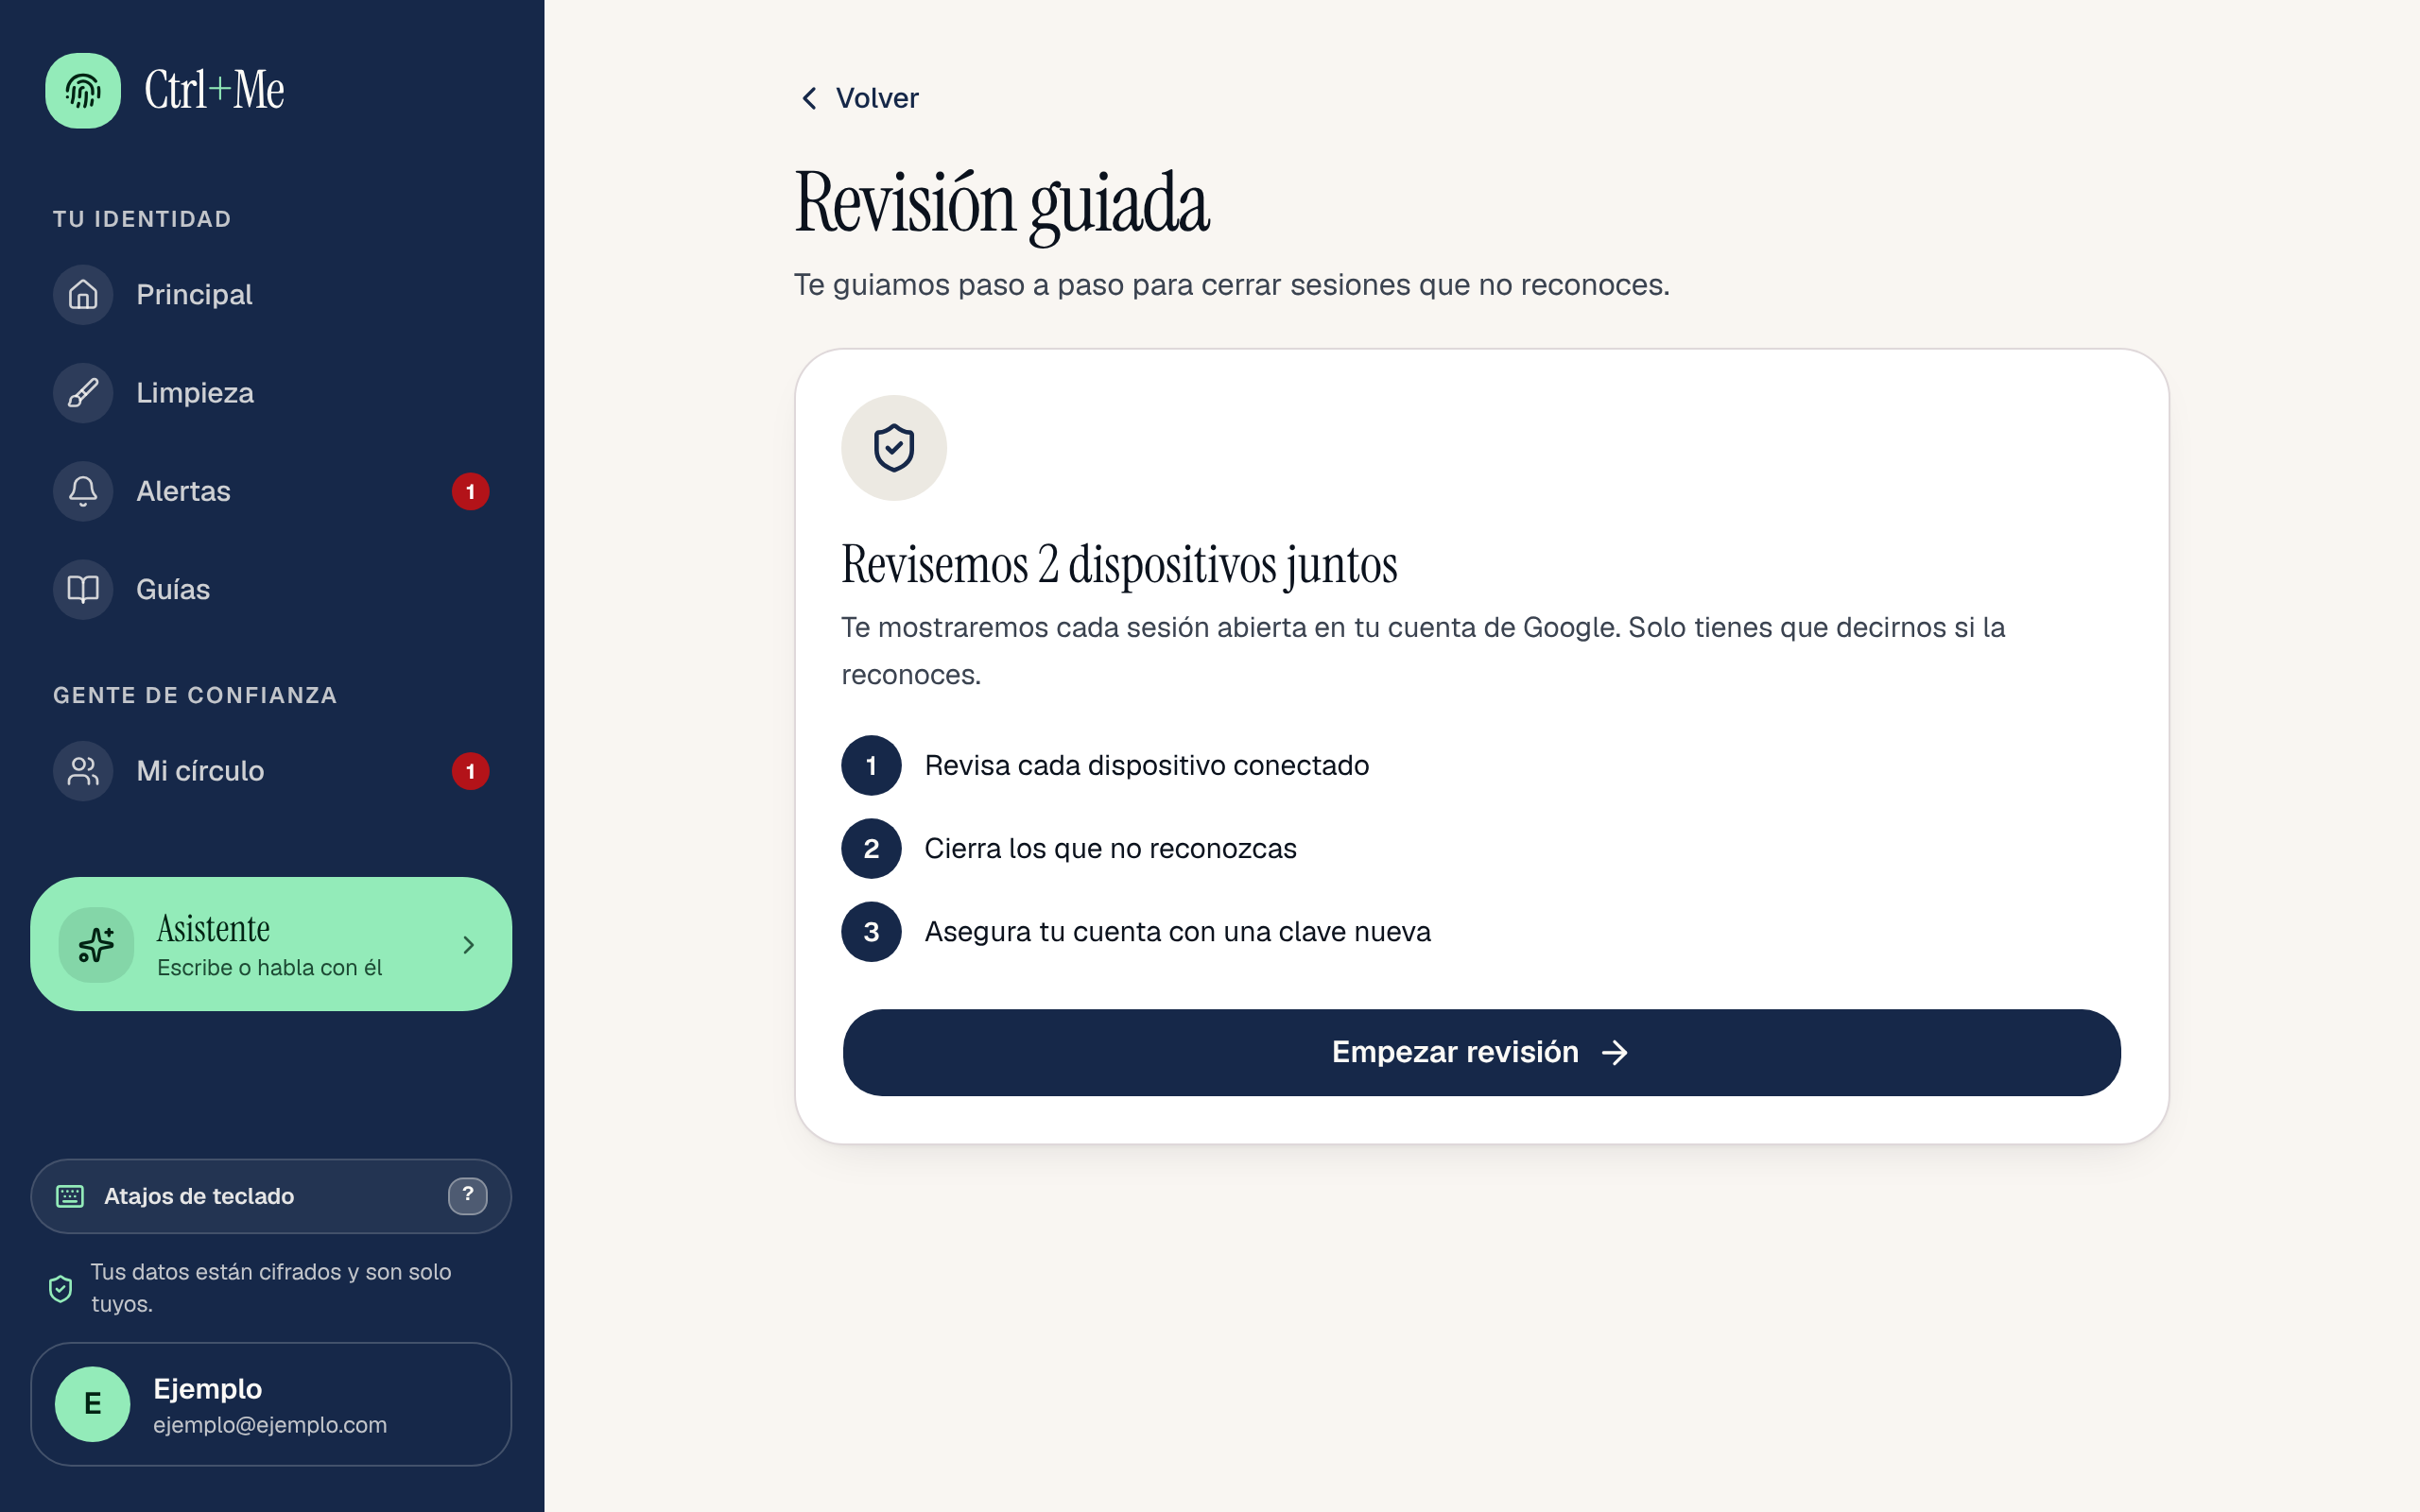
\includegraphics[width=\textwidth]{figuras-v3/v3_sesiones_web.png}
    \caption{Revisión guiada de sesiones desde el asistente (web)}
  \end{subfigure}
  \caption{Gestión de \textit{Mi círculo} con alto contraste, confirmaciones modales (\texttt{R-USA-6}) y revisión de sesiones.}
  \label{fig:v3-anexo-4}
\end{figure}
